\documentclass[11pt]{book}
\usepackage{csvsimple}
\usepackage{booktabs}
\usepackage[shortlabels]{enumitem}
\usepackage[section]{placeins}
\usepackage{graphicx}
\usepackage{makeidx}
\usepackage{xintbinhex}
%\usepackage{xintexpr}
\usepackage{hang}
\setlength{\parindent}{0pt}
\setlength{\parskip}{6pt}
\setlist{nosep}
\makeindex

\title{ZX Spectrum Next Programming Notes}
\date{\today}
\author{Theodore (Alex) Evans}
% custom sequences for consistency
\newcommand{\iis}{ I\textsuperscript{2}S }
\newcommand{\iic}{ I\textsuperscript{2}C }
\newcommand{\register}[3]{Register (#1) \$#2 (\xintHexToDec{#2}) $\Rightarrow$ #3}
\newcommand{\port}[2]{Port \$#1 (\xintHexToDec{#1}) #2}
\newcommand{\textoverline}[1]{$\overline{\hbox{#1}}$}
\begin{document}
\frontmatter
\maketitle
\tableofcontents
\mainmatter
Tile-sprite configuration (TSconf). Introduction

TS-Conf is a modern extension of the ZX Spectrum, which brings
long-awaited and features in the form of pixel oriented color,
hardware sprites, etc.

Graphic subsystem

Tao says: The screen we see is the output window of the resolution
specified in the system, which displays a block of 512x512 video
memory pages in the specified mode according to the given output
coordinates. TSU is a device that collects data from video, tile and
sprite memory, which processes and presents it at the current position
of the line drawing in a given resolution / desired mode.

This unit is an extension (add-on) above the standard 6912 byte
Spectrum screen. More precisely, the 6912 byte mode is part of the
whole family of system resolutions:
\begin{itemize}
\item 256x192
\item 320x200
\item 320x240
\item 360x288
\end{itemize}

These permissions can be used in different video modes:
\begin{itemize}
\item ZX
\item 16c
\item 256c
\item Text
\end{itemize}

To display the color for a given mode, the first block of the system's
internal memory is used - the palette memory . This block represents
512 bytes and stores the full color palette of the system - two-byte
data of color components for 256 colors.

The full palette is divided into groups of 16 colors (32 bytes) for
16c mode, which gives us 16 palettes with 16 colors.

The first palette is number 0. 

When you turn on the system, a set of 16 colors for the ZX mode is
loaded into the general palette, which is located in the last, 15th
palette.

Each mode sets its own characteristics of displaying color information
on the screen:
\begin{itemize}
\item ZX limits the output to the 16 colors of the standard ZX
  Spectrum palette;
\item 16c - in this mode only 16 colors are used - one of the 16
  available palettes;
\item 256c - provides the ability to display all the loaded colors in
  the palette
\item Text - text mode, allows you to display text in color.
\end{itemize}

In this case, it was a question of horizontal mobility. Let's talk
about vertical:

In addition to the listed modes, the system allows the use of layered
display of graphical information. The standard Spectrum screen is the
base screen, but it is not the lowest.

So, the location of the layers that form the screen: 
\begin{itemize}
\item[] 1. Border. A monochromatic fullscreen layer. Set the color of
  the border
\item[] 2. Basic (main) screen. May be included in any of the
  resolution/mode combinations
\item[] 3. Accelerated graphics layers displayed in the resolution
  specified for the base screen in 16 color mode
  \begin{itemize}
  \item sprite layer 0 
  \item tile layer 0 
  \item sprite layer 1 
  \item tile layer 1 
  \item sprite layer 2
  \end{itemize}
\end{itemize}

Thus, we have 7 layers that make up a single, visible screen.

All the layers use the colors specified in a common palette of 256
colors.

The tile and sprite layers only work in 16c mode, the 0th color of
each palette set is transparent. Thanks to TSU, there is no need to
save video memory data under tiles and sprites, since the display on
the screen is literally collected at the output of each line without
changing the contents of the video memory.

Each graphic element of these two types of layers represents a block
of at least 8x8 pixels, and for each of them it is necessary to
specify a palette, any one the available 16.

The tile layer is a map describing the location of the graphic
elements specified as an image. Thus, the position of the tile on the
screen directly depends on its position in the map.

Tile patterns: 64x64 tiles (4096 tiles in total), uses up to 4
palettes from 4 groups of all 16 palettes can be used for one
layer. For each tile it is possible to set its own (out of these 4)
palette.

In total, we have two such layers organized in the same way. 

Sprites are graphics, organized like tiles, but having large (multiple
of 8) sizes - from 8x8 to 64x64 pixels. Sprites also have zero color
transparency.

A feature of the sprites is that for each sprite, you can specify both
your its own palette and position to the pixel resolution.

The system uses the second block of internal memory to handle sprites,
representing the next 512 bytes of memory, which stores "sprite
handles"- data from 6 bytes, describing each sprite. The maximum
number of descriptors in this memory is 85 pieces.

In the following articles I will describe in more detail about working
with the devices listed at the beginning of the article.

PS: for those who do not want to wait and want details

\chapter{Video}

ZX Spectrum Next video splits the display types into four categories
(layer 1 (ULA/Timex/LoRes), layer 2, layer 3 (tilemap) and sprites)
which have their own sets of controls for colour palettes, clipping,
and scrolling. Some aspects of ULA and tilemap are tied together, but
all the rest operate in a largely independent manner using a layering
system. The ULA category has a number of separate video modes that it
can use. One of these (LoRes) is incompatible with using tilemaps.

\section{General Features}
There are a number of control features for the various video modes
that are done in a unified fashion. These features are layering and
transparency, palettes, scrolling, and clipping. 

\subsection{Video Layering and Transparency}
Video is rendered as three layers which are referred to as ULA (which
includes the tilemap), layer 2, and sprites.  The ordering of the
layers is controlled by Next port \$15 (21) bits 4-2:

\begin{table}[h]\centering
  \caption{Video Layering}
  \csvautotabular{video/videolayering.csv}
\end{table}

\index{transparency}
Transparency for Layer 2, ULA, LoRes, and 1-bit Tilemaps are
controlled by Next register \$14 (20) and defaults to \$E3. Sprites
and 4-bit Tilemaps have their own registers (\$4B and \$4C
respectively) for setting their transparency index (not colour). This
colour ignores the state of the least significant blue bit, so \$E3
equates to both \$1C6 and \$1C7. For Sprites and Tilemaps transparency
is determined by colour index. For Sprites this is controlled by
register \$4B (with only the least significant 4-bits being relevant
for 16-colour Sprites). For Tilemaps, the transparency index is set by
register \$4C. If all layers are transparent, the transparency
fallback colour is displayed. This is set by register \$4A.

(R/W) \$14 (20) $\Rightarrow$ Global Transparency Colour
\begin{itemize}
\item bits 7-0 = 8-bit transparency colour (soft reset = \$E3)
\end{itemize}

(R/W) \$4A (74) $\Rightarrow$ Fallback colour
\begin{itemize}
\item bits 7-0 = 8-bit colour used if all layers are transparent (soft
  reset = 0)
\end{itemize}

(R/W) \$4B (75) $\Rightarrow$ Sprite transparency index
\begin{itemize}
\item bits 7-0 = Sprite colour index treated as transparent (soft
  reset = \$E3)
\item[] For 4-bit sprites only the bottom 4-bits are used
\end{itemize}

(R/W) \$4C (74) $\Rightarrow$ Tilemap transparency index
\begin{itemize}
\item bits 7-4 = Reserved, must be 0
\item bits 3-0 = Tilemap colour index treated as transparent (soft
  reset \$f)
\end{itemize}

\subsection{Palette}
\index{palette}
\paragraph{Next Colour Palettes}
Each video mode group has a pair of palettes assigned to it a primary
and an alternate palette. Each palette entry is actually a 9-bit value
(RRRGGGBBB) and can be set by selecting a palette using nextreg \$43
(palette control), the entry using nextreg \$40 (palette index), then
writing the value into nextreg \$44 (palette value, 9-bit) using pairs
of consecutive writes for each palette value or nextreg \$41 (palette
value, 8-bit). Once a palette index has been selected writes
automatically increment the palette index number so it is possible to
efficiently write the values for a collection of palette entries.

(R/W) \$40 (64) $\Rightarrow$ Palette Index
\begin{itemize}
\item bits 7-0 = Select the palette index to change the associated
  colour. (soft reset = 0)
\item[] For the ULA only, INKs are mapped to indices 0-7, Bright INKS
  to indices 8-15, PAPERs to indices 16-23 and Bright PAPERs to
  indices 24-31.  In ULANext mode, INKs come from a subset of indices
  0-127 and PAPERs come from a subset of indices 128-255.  The number
  of active indices depends on the number of attribute bits assigned
  to INK and PAPER out of the attribute byte.  In ULA+ mode, the top
  64 entries hold the ula+ palette.  The ULA always takes border
  colour from paper for standard ULA and ULAnext.
\end{itemize}

(R/W) \$41 (65) $\Rightarrow$ Palette Value (8 bit colour)
\begin{itemize}
\item bits 7-0 = Colour for the palette index selected by nextreg
  \$40.
\item[] The format is RRRGGGBB - the lower blue bit of the 9-bit
  colour will be the logical OR of blue bits 1 and 0 of this 8-bit
  value.
\item[] After the write, the palette index is auto-incremented to the
  next index if the auto-increment is enabled in nextreg \$43.  Reads
  do not auto-increment.  Any other bits associated with the index
  will be zeroed.
\end{itemize}

(R/W) \$43 (67) $\Rightarrow$ Palette Control
\begin{itemize}
\item bit 7 = Disable palette write auto-increment (soft reset = 0)
\item bits 6-4 = Select palette for reading or writing (soft reset =
  000)
  \begin{itemize}
  \item 000 = ULA first palette
  \item 100 = ULA second palette
  \item 001 = Layer 2 first palette
  \item 101 = Layer 2 second palette
  \item 010 = Sprites first palette 
  \item 110 = Sprites second palette
  \item 011 = Tilemap first palette
  \item 111 = Tilemap second palette
  \end{itemize}
\item bit 3 = Select Sprites palette (0 = first palette, 1 = second
  palette) (soft reset = 0)
\item bit 2 = Select Layer 2 palette (0 = first palette, 1 = second
  palette) (soft reset = 0)
\item bit 1 = Select ULA palette (0 = first palette, 1 = second
  palette) (soft reset = 0)
\item bit 0 = Enable ULANext mode (soft reset = 0)
\end{itemize}

(R/W) \$44 (68) $\Rightarrow$ Palette Value (9 bit colour)
\begin{itemize}
\item[] Two consecutive writes are needed to write the 9 bit colour
\item[] 1st write:
\item bits 7-0 = RRRGGGBB
\item[] 2nd write:
\item bits 7-1 = Reserved, must be 0
\item bit 0 = lsb B
\item[] If writing to an L2 palette
\item bit 7 = 1 for L2 priority colour, 0 for normal.
\item[] An L2 priority colour moves L2 above all layers.  If you need
  the same colour in both priority and normal modes, you will need to
  have two different entries with the same colour one with and one
  without priority.  If auto-increment is enabled in nextreg \$43, the
  palette index is auto-incremented after two consecutive writes
\item[] Reads only return the 2nd byte and do not auto-increment.
\item[] can also be read back from nextreg \$28
\end{itemize}

\subsection{Scrolling}
The ZX Spectrum Next has four sets of scrolling registers to
independently contol the display offsets of various video modes
(Layer2, ULA, Tilemap, and LoRes). When the video is offset, the
portion that is pushed off the screen (to the left and or top) then
becomes visible on the opposite side of the screen so that the video
offset values are effectively the coordinates of the origin in a
toroidal universe.

\subsection{Clipping}
The ZX Spectrum Next has four clipping registers create a window of
the layer that is visible. Clipping is managed by a set of four
successive writes to the clipping register applicable for the video
mode. If a section is masked off by clipping, it is as if the area
were the transparency colour and the video lyers behind it become
visible.

\section{Layer 1}
The Layer 1 consists of ZX Spectrum ULA video, Timex video modes, and
the Spectrum Next’s lores video modes all use 16k memory bank 5 or 7
with the data coming from some combination of addresses \$0000-\$17FF
(bitmap 1), \$1800-\$1AFF (attribute 1), \$2000-\$37FF (bitmap 2), and
\$3800-\$3AFF (attribute 2) within the selected bank.  Assuming
default memory mapping and the use of bank 5 this will be mapped as
some combination of memory \$4000-\$57FF, \$5800-\$5AFF,
\$6000-\$77FF, \$780-\$7AFF. All of the modes other than the lores
mode can either use the default ZX Spectrum colours, ULANext mode, or
an emulation of ULAplus. In the Spectrum and Timex modes all colours are
either Paper (foreground), paper (background), or border colours.

\subsection{Colour Attributes}
The ZX Spectrum Next has three major modes for colour attributes: the
ZX Spectrum attribute mapping, which is augmented by using the ZX
Spectrum Next's palette; ULANext, which allows the user to how many
foreground and how many background colous are to be selected by the
attribute bytes; and an emulation of ULAplus.

\paragraph{ULA Colour}
In ULA colour INKs are mapped to indices 0-7, Bright INKS to indices
8-15, PAPERs to indices 16-23 and Bright PAPERs to indices 24-31. This
is the default state for interpreting ULA palettes.

\begin{table}[h]\centering
  \caption{ULA Colour}
  \csvautotabular{video/flash.csv}
\end{table}

\paragraph{ULANext}
The ULANext modes use a varying number of bits from the attribute
byte to determine the ink colours as the palette index from the
appropriate bits (all others being zero) and the paper colours coming
from the indicated value+128 with palette format 255 being a special
case where all the bits determine the ink colour while the paper is
always palette index 128. The ULA always takes border colour from
paper. ULANext is enabled using bit 0 of nextreg \$43 (palette
control) and controlled with nextreg \$42 (ULA Next attribute byte
format)

\begin{table}[h]\centering
  \caption{ULANext}
  \csvautotabular{video/palfmt.csv}
\end{table}

\paragraph{ULAplus}
The ZX Next emulates ULAPlus using the last 64 (192-255) entries of
the ULA palette. ULAplus is controlled using two ports: \$BF3B (register
port) and \$FF3B (data port)

\subparagraph{I/O ports}
ULAplus is controlled by two ports.

\$BF3B is the register port (write only)

The byte output will be interpreted as follows:
\begin{itemize}
\item Bits 7-6: Select the register group. Two groups are currently available:
  \begin{itemize}
  \item 00=palette group\\
    When this group is selected, the sub-group determines the entry in the
    palette table (0-63).
  \item 01=mode group\\
    The sub-group is (optionally) used to mirror the video functionality
    of Timex port \$FF as follows:
  \end{itemize}
\item Bits 5-0: Select the register sub-group
\item[] Mode group
\item Bits 5-3: Sets the screen colour in hi-res mode.
  \begin{itemize}
  \item 000=Black on White
  \item 001=Blue on Yellow
  \item 010=Red on Cyan
  \item 011=Magenta on Green
  \item 100=Green on Magenta
  \item 101=Cyan on Red
  \item 110=Yellow on Blue
  \item 111=White on Black
  \end{itemize}
\item Bits 2-0: Screen mode.
  \begin{itemize}
  \item 000=screen 0 (bank 5)
  \item 001=screen 1 (bank 5)
  \item 010=hi-colour (bank 5)
  \item 100=screen 0 (bank 7)
  \item 101=screen 1 (bank 7)
  \item 110=hi-colour (bank 7)
  \item 110=hi-res (bank 5)
  \item 111=hi-res (bank 7)
  \end{itemize}
\end{itemize}

\$FF3B is the data port (read/write)

When the palette group is selected, the byte written will describe the
color.

When the mode group is selected, the byte output will be interpreted
as follows:
\begin{itemize}
\item Bit 0: ULAplus palette on (1) / off (0)
\item Bit 1: (optional) grayscale: on (1) / off (0) (same as turing
  the color off on the television)
\end{itemize}

Implementations that support the Timex video modes use the \$FF
register as the primary means to set the video mode, as per the Timex
machines. It is left to the individual implementations to determine if
reading the port returns the previous write or the floating bus.

\subparagraph{GRB palette entries}

G3R3B2 encoding\\
For a device using the GRB colour space the palette entry is
interpreted as follows
\begin{itemize}
\item Bits 7-5: Green intensity.
\item Bits 4-2: Red intensity.
\item Bits 1-0: Blue intensity.
\end{itemize}

This colour space uses a sub-set of 9-bit GRB. The missing lowest blue
bit is set to OR of the other two blue bits (Bb becomes 000 for 00,
and Bb1 for anything else). This gives access to a fixed half the
potential 512 colour palette. The reduces the jump in intensity in the
lower range in the earlier version of the specification. It also means
the standard palette can now be represented by the ULAplus palette.

\subparagraph{Grayscale palette entries}
In grayscale mode, each palette entry describes an intensity from zero
to 255. This can be achieved by simply removing the colour from the
output signal.

\subparagraph{Limitations}
Although in theory 64 colours can be displayed at once, in practice
this is usually not possible except when displaying colour bars,
because the four CLUTs are mutually exclusive; it is not possible to
mix colours from two CLUTs in the same cell. However, with software
palette cycling it is possible to display all 256 colours on screen at
once.

\subparagraph{Emulation}
The 64 colour mode lookup table is organized as 4 palettes of 16
colours.

Bits 7 and 6 of each Spectrum attribute byte (normally used for FLASH
and BRIGHT) will be used as an index value (0-3) to select one of the
four colour palettes.

Each colour palette has 16 entries (8 for INK, 8 for PAPER). Bits 0 to
2 (INK) and 3 to 5 (PAPER) of the attribute byte will be used as
indexes to retrieve colour data from the selected palette.

With the standard Spectrum display, the BORDER colour is the same as
the PAPER colour in the first CLUT. For example BORDER 0 would set the
border to the same colour as PAPER 0 (with the BRIGHT and FLASH bits
not set).

The complete index can be calculated as\\
ink\_colour = (FLASH * 2 + BRIGHT) * 16 + INK
paper\_colour = (FLASH * 2 + BRIGHT) * 16 + PAPER + 8

\subparagraph{Palette file format}
The palette format doubles as the BASIC patch loader. This enables you
to edit patches produced by other people.
\begin{verbatim}
; 64 colour palette file format (internal) - version 1.0
; copyright (c) 2009 Andrew Owen
;
; The palette file is stored as a BASIC program with embedded machine code

header:

db 0x00 ; program file
db 0x14, 0x01, "64colour" ; file name
dw 0x0097 ; data length
dw 0x0000 ; autostart line
dw 0x0097 ; program length

basic:

; 0 RANDOMIZE USR ((PEEK VAL "2
; 3635"+VAL "256"*PEEK VAL "23636"
; )+VAL "48"): LOAD "": REM

db 0x00, 0x00, 0x93, 0x00, 0xf9, 0xc0, 0x28, 0x28
db 0xbe, 0xb0, 0x22, 0x32, 0x33, 0x36, 0x33, 0x35
db 0x22, 0x2b, 0xb0, 0x22, 0x32, 0x35, 0x36, 0x22
db 0x2a, 0xbe, 0xb0, 0x22, 0x32, 0x33, 0x36, 0x33
db 0x36, 0x22, 0x29, 0x2b, 0xb0, 0x22, 0x34, 0x38
db 0x22, 0x29, 0x3a, 0xef, 0x22, 0x22, 0x3a, 0xea

start:

di ; disable interrupts
ld hl, 38 ; HL = length of code
add hl, bc ; BC = entry point (start) from BASIC
ld bc, 0xbf3b ; register select
ld a, 64 ; mode group
out (c), a ;
ld a, 1 ;
ld b, 0xff ; choose register port
out (c), a ; turn palette mode on
xor a ; first register

setreg:

ld b, 0xbf ; choose register port
out (c), a ; select register
ex af, af' ; save current register select
ld a, (hl) ; get data
ld b, 0xff ; choose data port
out (c), a ; set it
ex af, af' ; restore current register
inc hl ; advance pointer
inc a ; increase register
cp 64 ; are we nearly there yet?
jr nz, setreg ; repeat until all 64 have been done
ei ; enable interrupts
ret ; return

; this is where the actual data is stored. The following is an example palette.

registers:

db 0x00, 0x02, 0x18, 0x1b, 0xc0, 0xc3, 0xd8, 0xdb ; INK
db 0x00, 0x02, 0x18, 0x1b, 0xc0, 0xc3, 0xd8, 0xdb ; PAPER
db 0x00, 0x03, 0x1c, 0x1f, 0xe0, 0xe3, 0xfc, 0xff ; +BRIGHT
db 0x00, 0x03, 0x1c, 0x1f, 0xe0, 0xe3, 0xfc, 0xff ;
db 0xdb, 0xd8, 0xc3, 0xc0, 0x1b, 0x18, 0x02, 0x00 ; +FLASH
db 0xdb, 0xd8, 0xc3, 0xc0, 0x1b, 0x18, 0x02, 0x00 ;
db 0xff, 0xfc, 0xe3, 0xe0, 0x1f, 0x1c, 0x03, 0x00 ; +BRIGHT/
db 0xff, 0xfc, 0xe3, 0xe0, 0x1f, 0x1c, 0x03, 0x00 ; +FLASH

terminating_byte:

db 0x0d 
\end{verbatim}

\subsection{Layer 1 Scrolling}
Layer 1 has two sets of scrolling registers. One for the the legacy
modes (ZX Spectrum, Alternate Page, Timex Hi-Resoulution, and Timex
Hi-colour) and a second set for the two ZX Spextrum Next specific
LoRes modes.  All modes scroll as if they were $256\times192$ screens
located at global coordinates (32, 32) to (287, 223), The registers
for the legacy modes are \$26 and \$27 and the registers for the LoRes
modes are \$32 and \$33.

\register{R/W}{26}{ULA Horizontal Scroll Control}
\begin{itemize}
\item bits 7-0 = ULA X Offset (0-255) (0 on reset)
\end{itemize}


\register{R/W}{27}{ULA Vertical Scroll Control}
\begin{itemize}
\item bits 7-0 = ULA Y Offset (0-191) (0 on reset)
\end{itemize}


\register{R/W}{32}{Layer 1,0 (LoRes) Horizontal Scroll Control)}
\begin{itemize}
\item bits 7-0 = X Offset (0-255) (\$00 on reset)
\end{itemize}
Layer 1,0 (LoRes) scrolls in "half-pixels" at the same resolution and
smoothness as Layer 2.


\register{R/W}{33}{Layer 1,0 (LoRes) Vertical Scroll Control)}
\begin{itemize}
\item bits 7-0 = Y Offset (0-191) (\$00 on reset)
\end{itemize}
Layer 1,0 (LoRes) scrolls in "half-pixels" at the same resolution and
smoothness as Layer 2.



\subsection{Layer 1 Clipping}
All of the modes in the Layer 1 share a single clipping register,
\$1A. The clip index may alternately be set using register \$1C. This
is expecially useful for reading the current clipping coordinates as
reads on the clipping register do not change the index. Note that
clipping coordinates are based on a full display area for the mode of
$256\times192$ resolution even though not all modes have that
resolution.

\register{R/W}{1A}{Layer 0 (ULA/LoRes) Clip Window Definition}
\begin{itemize}
\item bits 7-0 = Coord. of the clip window
  \begin{itemize}
  \item[] 1st write = X1 position
  \item[] 2nd write = X2 position
  \item[] 3rd write = Y1 position
  \item[] 4rd write = Y2 position
  \end{itemize}
\end{itemize}
The values are 0,255,0,191 after a Reset\\
Reads do not advance the clip position


\register{R/W}{1C}{Clip Window Control}\\
Read
\begin{itemize}
\item bits 7-6 = Layer 3 Clip Index
\item bits 5-4 = Layer 0/1 Clip Index
\item bits 3-2 = Sprite clip index
\item bits 1-0 = Layer 2 Clip Index
\end{itemize}
Write
\begin{itemize}
\item bits 7-4 = Reserved, must be 0
\item bit 3 - reset Layer 3 clip index
\item bit 2 - reset Layer 0/1 clip index
\item bit 1 - reset sprite clip index.
\item bit 0 - reset Layer 2 clip index.
\end{itemize}



\subsection{ZX Spectrum Mode}

Timex mode 0

This is the default ULA mode and has its origins in the original ZX
Spectrum. It uses $256\times192$ pixels located at global coordinates
(32, 32) to (287, 223) with $8\times8$ colour attribute areas mapped
into a $32\times24$ grid. If Timex modes are not enabled, this and the
LoRes mode are the only ones available, so you would switch back to
this mode by writing 000xxxxx to Next register \$15 (21, the sprites
and layers register). If another Timex mode is enabled, then this is
mode 0 so you would write 0 to port \$ff to enable it. This is a
$256\times192$ video mode. The bitmap 1 area is used for selection
between ink and paper colours with one bit per pixel and the attribute
1 area for colour attributes.

The easiest way to visualize the mapping of this mode is to think of
the $256\times192$ area as being divided into a $32\times24$ grid of
$8\times8$ characters.  IF we consider X and Y as the position in the
grid and R to the the row within the character.  For ink/paper
selection, 0=paper, 1=ink and the entries are stored left to right as
lsb to msb within the bye.  The address for a pixel value is:
$0R_4R_3Y_2Y_1Y_0R_2R_1R_0C_4C_3C_2C_1C_0$. Each $8\times8$ cell has
its own colour attribute where the address for an attribute cell is
$0110R_4R_3R_2R_1R_0C_4C_3C_2C_1C_0$ in other words mapped lineally
column-wise starting at the beginning of the attribute 1 area.

Code:
\begin{verbatim}
  ;; from any other Timex mode:
  ld a,$00
  ld c,$ff
  out (c),a

  ;; from LoRes mode:
  ld bc,$243B ; next register select port
  ld a,$15
  out (c),a
  ld bc,$253B ; next register r/w port
  in a,(c)
  and $7f
  out (c),a
\end{verbatim}

\subsection{Alternate Page Mode}

Timex mode 1

This mode is the same as ZX Spectrum mode except it is at an alternate
addresses. Alternate page mode is selected by enabling Timex modes by
writing 00xxxx1xx to Next register \$08 (8, Peripheral 3 setting) then
writing 1 to the Timex ULA port (\$ff).  It is identical to ZX
Spectrum mode except the pixel are mapped to the bitmap 2 area giving
use pixel addresses of $1R_4R_3Y_2Y_1Y_0R_2R_1R_0C_4C_3C_2C_1C_0$ and
the attributes to the attribute 2 area with addresses of
$1110R_4R_3R_2R_1R_0C_4C_3C_2C_1C_0$.

Code:

\begin{verbatim}
;; disable LoRes mode:
ld bc,$243B ; next register select port
ld a,$15
out (c),a
ld bc,$253B ; next register r/w port
in a,(c)
and $7f
out (c),a
;; set Timex mode
ld bc,$243B ; next register select port
ld a,$08
out (c),a
ld bc,$253B ; next register r/w port
in a,(c)
or $04
out (c),a
;; set alternate page mode
ld c,$ff
ld a,$01
out (c),a
\end{verbatim}

\subsection{Timex Hi-Colour Mode}

Timex mode 2

This mode is a $256\times192$ video mode located at global coordinates
(32, 32) to (287, 223) with $8\times1$ colour attribute mapping on a
$32\times192$ grid. It is selected by writing 2 to the Timex ULA port
(\$ff).  Pixel mapping in this mode is the same as in ZX Spectrum mode
using the bitmap 1 area based on
$0R_4R_3Y_2Y_1Y_0R_2R_1R_0C_4C_3C_2C_1C_0$.  The colour attributes use
the bitmap 2 area with $8\times1$ colour attribute areas corresponding
to the addresses $1R_4R_3Y_2Y_1Y_0R_2R_1R_0C_4C_3C_2C_1C_0$.

Code:
\begin{verbatim}
;; disable LoRes mode:
ld bc,$243B ; next register select port
ld a,$15
out (c),a
ld bc,$253B ; next register r/w port
in a,(c)
and $7f
out (c),a
;; set Timex mode
ld bc,$243B ; next register select port
ld a,$08
out (c),a
ld bc,$253B ; next register r/w port
in a,(c)
or $04
out (c),a
;; set hi-colour mode
ld c,$ff
ld a,$02
out (c),a
\end{verbatim}

\subsection{Timex Hi-Resolution Mode}

Timex mode 6

This is a monochrome $512\times192$ video mode located at global
coordinates (32, 32) to (287, 223) with each pixel being half
width. It is selected by writing to the Timex ULA port (\$ff with
values that also select which two colours (or colour entries in
ULANext mode) you use.

\begin{table}[h]\centering
  \caption{Hi-Resolution Colours}
  \csvautotabular{video/hires.csv}
\end{table}
  
Pixels are mapped into both the bitmap 1 and bitmap 2 areas where
8-pixel wide character columns alternate between the two bitmap areas.
The pixels within a byte being rendered left to right lsb to msb as in
other Spectrum video modes.  The addresses for each row within a
character are based on a $64\times32$ grid of $8\times8$ characters
which using a $64\times24$ R, C, and Y scheme gives us addresses of
the form $C_0R_4R_3Y_2Y_1Y_0R_2R_1R_0C_5C_4C_3C_2C_1$.

Code:
\begin{verbatim}
;; disable LoRes mode:
ld bc,$243B ; next register select port
ld a,$15
out (c),a
ld bc,$253B ; next register r/w port
in a,(c)
and $7f
out (c),a
;; set Timex mode
ld bc,$243B ; next register select port
ld a,$08
out (c),a
ld bc,$253B ; next register r/w port
in a,(c)
or $04
out (c),a
;; set hi-res mode, black on white
ld c,$ff
ld a,$06
out (c),a
\end{verbatim}

\subsection{Lo-Resolution Mode}
This is a Spectrum Next specific video mode with a resolution of
$128\times96$ located at global coordinates (32, 32) to (287, 223)
with each pixel being double height and double width replacing the old
Radistan mode.  It can either allow for 16 colours, in which case it
uses either the bitmap 1 area or the bitmap 2 area, or 256 colours
using both bitmap 1 and bitmap 2. The colour of each pixel can be
selected independently with data ordered linearly in a row major
fashion. In the case of 16 colour mode, the nybbles describing the
colours are X major (MSN LSN). Scrolling is by half pixels and uses
different registers (\$32 and \$33) from the rest of the ULA group
modes. LoRes mode is enabled by writing $100xxxxx$ to Next register
\$15 (the sprites and layers register) with Next register \$6A used to
decide whether it is 16 or 256 colours.

\register{R/W}{15}{Sprite and Layer System Setup}
\begin{itemize}
\item bit 7 = LoRes mode (0 on reset)
\item bit 6 = Sprite priority (1 = sprite 0 on top, 0 = sprite 127 on
  top) (0 on reset)
\item bit 5 = Enable sprite clipping in over border mode (0 on reset)
\item bits 4-2 = set layers priorities (000 on reset)
  \begin{itemize}
  \item 000 - S L U
  \item 001 - L S U
  \item 010 - S U L
  \item 011 - L U S
  \item 100 - U S L
  \item 101 - U L S
  \item 110 - S(U+L) ULA and Layer 2 combined, colours clamped to 7
  \item 111 - S(U+L-5) ULA and Layer 2 combined, colours clamped to [0,7]
  \end{itemize}
\item bit 1 = Enable Sprites Over border (0 on reset)
\item bit 0 = Enable Sprites (0 on reset)
\end{itemize}


\register{R/W}{32}{Layer 1,0 (LoRes) Horizontal Scroll Control)}
\begin{itemize}
\item bits 7-0 = X Offset (0-255) (\$00 on reset)
\end{itemize}
Layer 1,0 (LoRes) scrolls in "half-pixels" at the same resolution and
smoothness as Layer 2.


\register{R/W}{33}{Layer 1,0 (LoRes) Vertical Scroll Control)}
\begin{itemize}
\item bits 7-0 = Y Offset (0-191) (\$00 on reset)
\end{itemize}
Layer 1,0 (LoRes) scrolls in "half-pixels" at the same resolution and
smoothness as Layer 2.


\register{R/W}{6A}{Layer 1,0 (LoRes) Control}
\begin{itemize}
\item bits 7-6 = reserved, must be 0
\item bit 5 = Enable Radistan (16-colour) (0 on reset)
\item bit 4 = Radistan DFILE switch (xor with bit 0 of port \$ff) (0
  on reset)
\item bits 3-0 = Radistsan palette offset (0 on reset)
\item bits 1-0 = ULAplus palette offset (0 on reset)
\end{itemize}



Code: 256 colour
\begin{verbatim}
;; enable LoRes mode:
nextreg $15,$80
;; 256-colour mode
ld bc,$243B ; next register select port
ld a,$6A
out (c),a
ld bc,$253B ; next register r/w port
in a,(c)
and $EF ; lores radistan control
out (c),a
\end{verbatim}

Code: 16 colour
\begin{verbatim}
;; enable LoRes mode:
nextreg $15,$80
;; 16-colour mode
nextreg $6A,$10
\end{verbatim}

\section{Layer 2}
Layer 2 is a linearly mapped, row-wise, upper left to lower right,
bit-map graphics area.  It supports modes with $256\times192\times256$
resolution at global coordinates (32, 32) to (287, 223),
$320\times256\times256$ resolution at global coordinates (0, 0) to
(318, 255), and $640\times256\times16$ resolution at global
coordinates (0, 0) to (319, 255) with half width pixels. It can be
mapped starting at any 16k memory blocks. The $256\times192\times256$
mode requires 3 consecutive blocks (48k) while the others use 5
consecutive blocks (80k).

\subsection{Configuration}
Layer 2 is enabled using port \$123B or register \$69. The mode is
selected using register \$70. How layer 2 memory is overlaid on main
memory is controled by port \$123B and register \$70. The location in
memory is controlled by register \$12 with a shadow area pointed to by
register \$13 for double buffering. Finally port \$123B is used to
select either the main RAM area or the shadow RAM area for rendering
the layer.

\port{123B}{Layer 2}\\
Bit 4 = 0
\begin{itemize}
\item[] bits 7-6 = Video RAM bank select
  \begin{itemize}
  \item[] 00 = first 16k
  \item[] 01 = second 16k
  \item[] 10 = third 16k
  \item[] 11 = first 48k
  \end{itemize}
\item[] bit 5 = Reserved, must be 0
\item[] bit 4 = 0
\item[] bit 3 = Shadow layer 2 select
\item[] bit 2 = Enable layer 2 read paging
\item[] bit 1 = Layer 2 visible (mirrored in register \$69)
\item[] bit 0 = Enable layer 2 write paging
\end{itemize}
Bit 4 = 1
\begin{itemize}
\item[] bits 7-5 = Reserved, must be 0
\item[] bit 4 = 1
\item[] bit 3 = Reserved, must be 0
\item[] bit 2-0 = 16k bank relative offset
\end{itemize}


\register{R/W}{12}{Layer 2 Active RAM bank}
\begin{itemize}
\item bits 7-6 = Reserved, must be 0
\item bits 5-0 = RAM bank (point to bank 8 after a Reset, NextZXOS
  modifies to 9)
\end{itemize}


\register{R/W}{13}{Layer 2 Shadow RAM bank}
\begin{itemize}
\item bits 7-6 = Reserved, must be 0
\item bits 5-0 = RAM bank (point to bank 11 after a Reset, NextZXOS
  modifies to 12)
\end{itemize}


\register{R/W}{69}{Display Control 1}
\begin{itemize}
\item bit 7 = Layer 2 Enable (Port \$123B bit 1 alias)
\item bit 6 = ULA Shadow display enable (Port \$7FFD bit 3 alias)
\item bits 5-0 = Timex alias (Port \$FF alias)
\end{itemize}


\register{R/W}{70}{Layer 2 Control}
\begin{itemize}
\item bits 7-6 = Reserved, must be 0
\item bits 5-4 = Resolution (00 on soft reset)
  \begin{itemize}
  \item 00 = $256\times192\times256$
  \item 01 = $320\times256\times256$
  \item 10 = $640\times256\times16$
  \item 11 = Do not use
  \end{itemize}
\item bits 3-0 = Palette offset (\$0 on soft reset)
\end{itemize}


\sinset
Code:
\paragraph{Layer 2 $256\times192$, Write only overlaid on ROM}
\begin{verbatim}
p_layer2: defl $123b
start:
  ld bc,p_layer2
  ld a,$03       ; enable, wo, 1st 16k
  out (c),a
  call wrtpage
  ld bc,p_layer2
  ld a,$43       ; enable, wo, 2nd 16k
  out (c),a
  call wrtpage
  ld bc,p_layer2
  ld a,$83       ; enable, wo, 3rd 16k
  out (c),a
  call wrtpage
  ret
wrtpage:  
  ld hl,$0000
  ld bc,$0040    ; 40*256 writes
loop:
  ld (hl),b
  inc hl
  djnz loop
  dec c
  jr nz,loop
\end{verbatim}
\paragraph{Layer 2 $256\times192$ resolution}
\begin{verbatim}
r_mmu_7:  defl $57
r_disp1:  defl $69
r_layer2: defl $70
start:
  nextreg r_disp1,$80  ; enable layer 2
  nextreg r_layer2,$00 ; 256x192x256
  ld a,$12             ; page 18=bank 9
loop1:
  nextreg r_mmu_7,a    ; map page into slot 7
  ld bc,$0020          ; 20*256 = 8k
  ld hl,$E000          ; address of slot 7
loop2:
  ld (hl),b
  inc hl
  djnz loop2
  dec c
  jp NZ,loop2
  inc a
  cp $18               ; stop at page 24
  jp NZ,loop1
\end{verbatim}
\paragraph{Layer 2 $320\times256$ resolution}
\begin{verbatim}
r_mmu_7:  defl $57
r_disp1:  defl $69
r_layer2: defl $70
start:
  nextreg r_disp1,$80  ; enable layer 2
  nextreg r_layer2,$10 ; 320x256x256
  ld a,$12             ; page 18=bank 9
loop1:
  nextreg r_mmu_7,a    ; map page into slot 7
  ld bc,$0020          ; 20*256 = 8k
  ld hl,$E000          ; start of slot 7
loop2:
  ld (hl),b
  inc hl
  djnz loop2
  dec c
  jp NZ,loop2
  inc a
  cp $1C               ; stop at page 28
  jp NZ,loop1
\end{verbatim}
\paragraph{Layer 2 $640\times256$ resolution}
\begin{verbatim}
r_mmu_7:  defl $57
r_disp1:  defl $69
r_layer2:  defl $70
start:
  nextreg r_disp1, $80   ; enable layer 2
  nextreg r_layer2, $20  ; 640x256x16
  ld a, $12    ; page 18=bank 9
loop1:
  nextreg r_mmu_7, a  ; map page into slot 7
  ld bc, $0020    ; 20*256 = 8k
  ld hl, $E000    ; start address for slot 7
loop2:
  ld (hl), b
  inc hl
  djnz loop2
  dec c
  jp NZ, loop2
  inc a
  cp $1C      ; stop at page 28
  jp NZ, loop1
\end{verbatim}
\einset

\subsection{Scrolling}
Scrolling Layer 2 is controlled by registers \$16 and \$17. (Is there
a third scrolling register for layer 2?)

\register{R/W}{16}{Layer 2 Horizontal Scroll Control}
\begin{itemize}
\item bits 7-0 = X Offset (0-255)(0 on reset)
\end{itemize}


\register{R/W}{17}{Layer 2 Vertical Scroll Control}
\begin{itemize}
\item bits 7-0 = Y Offset (0-191)(0 on reset)
\end{itemize}



\subsection{Clipping}
The Clip area for is based on the local coordinate system for the mode
in question and is set using register \$18 with the option of
selection which write in active using register \$1C.

\register{R/W}{18}{Layer 2 Clip Window Definition}
\begin{itemize}
\item bits 7-0 = Coords of the clip window
  \begin{itemize}
  \item[] 1st write - X1 position
  \item[] 2nd write - X2 position
  \item[] 3rd write - Y1 position
  \item[] 4rd write - Y2 position
  \end{itemize}
\end{itemize}
Reads do not advance the clip position\\
The values are 0,255,0,191 after a Reset


\register{R/W}{1C}{Clip Window Control}\\
Read
\begin{itemize}
\item bits 7-6 = Layer 3 Clip Index
\item bits 5-4 = Layer 0/1 Clip Index
\item bits 3-2 = Sprite clip index
\item bits 1-0 = Layer 2 Clip Index
\end{itemize}
Write
\begin{itemize}
\item bits 7-4 = Reserved, must be 0
\item bit 3 - reset Layer 3 clip index
\item bit 2 - reset Layer 0/1 clip index
\item bit 1 - reset sprite clip index.
\item bit 0 - reset Layer 2 clip index.
\end{itemize}



\section{Layer 3 (Tilemap) Mode}

Started with documentation by Phoebus Dokos, February 25,
2019. Partially rewritten for clarity and to add core 3.00.00
features.

\subsection{General Description}
The tilemap is a hardware character oriented display. It uses a set of
user defined 4-bit, 16-colour, or 1-bit, 2-colour $8\times8$
tiles. The tiles can be dispplayed in two resolutions: $40\times32$
tiles ($320\times256$ pixels) and $80\times32$ tiles ($640\times256$
pixels).

The display area on screen is the same as the sprite layer, meaning it
overlaps the standard $256\times192$ area by 32 pixels on all
sides. Vertically this is larger than the physical HDMI display, which
will cut off the top and bottom character rows making the visible area
$40\times30$ or $80\times30$, but the full area is visible on VGA.

The obvious application for the tilemap is for a fast, clearly
readable and wide multicoloured character display. Less obvious
perhaps is that it can also be used to make fast and wide resolution
full colour backgrounds with easily animated components such as have
historically been used in many games.

The tilemap is defined by two data structures and configured using
four NextRegs. The NextRegs are \$6b (107), Tilemap Control; \$6c
(108), Default Tilemap Attribute, \$6c (110); Tilemap Base Address;
and \$6d (111) Tile Definitions Base Address.

\subsection{Data Structures}

\paragraph{Tilemap}

The first data structure is the tilemap itself which indicates what
characters occupy each cell on screen. Each tilemap entry is either
one or two bytes.

If entries are two bytes each, the first byte for each entry is bits
0-7 of the tile number, while the second byte is an attribute byte
which is interpreted acctording to the mode set in the tilemap control
register (\$6b). For $40\times32$ resolution, a full size tilemap will
occupy 2560 bytes, and for $80\times32$ resolution the space taken is
twice that at 5120 bytes. The tilemap entries are stored in X-major
order and each two-byte tilemap entry consists of a tile number byte
(bits 0-7 of the tile number) followed an attribute byte:

Tilemap Attribute Byte 4-bit
\begin{itemize}
\item[] bits 7-4 : most significant 4-bits of palette entry
\item[] bit 3 : x mirror
\item[] bit 2 : y mirror
\item[] bit 1 : rotate
\item[] bit 0 : ULA over tilemap (in 512 tile mode, bit 8 of the tile
  number)
\end{itemize}

Tilemap Attribute Byte 1-bit
\begin{itemize}
\item[] bits 7-1 : most significan 7-bits of palette entry
\item[] bit 0 : ULA over tilemap (in 512 tile mode, bit 8 of the tile
  number)
\end{itemize}

The character displayed is indicated by the “tile number” which can be
thought of as an ASCII code. The tile number is normally eight bits
allowing up to 256 unique tiles to be displayed but this can be
extended to nine bits for 512 unique tiles if 512 tile mode is enabled
via the Tilemap Control register (\$6b).

The other bits are tile attributes that modify how the tile image is
drawn. Their function is the same as the equivalent sprite attributes
for sprites. Bits apply rotation then mirroring, and colour can be
shifted with a palette offset. If 512 tile mode is not enabled, bit 8
will determine if the tile is above or below the ULA display on a per
tile basis.

When using 1-byte tilemap entries, the map consists of the tile
numbers for tile in the map with the tilemap attribute byte for every
tile coming from the default tilemap attribute register (\$6c).

\paragraph{Tile Definitions}
The second data structure is the tile definitions themselves. To find
the difinition for a specific tile you would look at (base address) +
(tile number) * (definition size).

For 4-bit, 16-colour, tiles, each $8\times8$ tile takes up 32
bytes. Each pixel uses four bits to select one of 16 colours. A tile
is defined in X major order with packing in the X direction in the
same way that 4-bit sprites are defined. The 4-bit colour of each
pixel is augmented by the 4-bit palette offset from the tilemap in the
most significant bits to form an 8-bit colour index that is looked up
in the tilemap palette to determine the final 9-bit colour sent to the
display. Ane of the 16 colours for each tile is the transparency
color.

For 1-bit, 2-colour, tiles, each $8\times8$ tile takes up 8
bytes. Each pixel uses one bit to select one of two colours. A tile is
defined in X major order with packing in the X direction. The 1-bit
colour of each pixel is augmented by the 7-bit palette offset from the
tilemap in the most significant bits to form an 8-bit colour index
that is looked up in the tilemap palette to determine the final 9-bit
colour sent to the display. Transparency for each tile is according to
the global transparency colour.

\subsection{Memory Organization \& Display Layer}
The tilemap is a logical extension of the ULA and its data structures
are contained in the ULAís 16k bank 5. If both the ULA and tilemap are
enabled, this means that the tilemapís map and tile definitions should
be arranged within the 16k to avoid overlap with the display ram used
by the ULA.

The tilemap exists on the same display layer as the ULA. The graphics
generated by the ULA and tilemap are combined before being forwarded
to the SLU layer system as layer U.

\subsection{Combining ULA \& Tilemap}
The combination of the ULA and tilemap is done in one of two modes:
the standard mode or the stencil mode.

The standard mode uses bit 8 of a tile's tilemap entry to determine if
a tile is above or below the ULA. The source of the final pixel
generated is then the topmost non-transparent pixel. If the ULA or
tilemap is disabled then they are treated as transparent.

The stencil mode will only be applied if both the ULA and tilemap are
enabled. In the stencil mode, the final pixel will be transparent if
either the ULA or tilemap are transparent. Otherwise the final pixel
is a logical AND of the corresponding colour bits. The stencil mode
allows one layer to act as a cut-out for the other.

\subsection{Programming Tilemap mode}

(R/W) \$6B (107) $\Rightarrow$ Tilemap Control
\begin{itemize}
\item[] bit 7    = 1 to enable the tilemap
\item[] bit 6    = 0 for $40\times32$, 1 for $80\times32$
\item[] bit 5    = 1 to eliminate the attribute entry in the tilemap
\item[] bit 4    = palette select
\item[] bit 3    = 0 for 16-colour, 1 for 2-colour
\item[] bit 2    = Reserved set to 0
\item[] bit 1    = 1 to activate 512 tile mode
\item[] bit 0    = 1 to force tilemap on top of ULA
\end{itemize}

Bits 7 \& 6 enable the tilemap and select resolution. Bit 4 selects one
of two tilemap palettes used for final colour lookup. Bit 5 changes
the structure of the tilemap so that it contains only 8-bit tilemap
entries instead of 16-bit tilemap entries. If 8-bit, the tilemap only
contains tile numbers and the attributes are instead taken from
nextreg \$6C.

Bit 5 determines whether the attribute byte for each tile come from
the tilemap (0) or from the default tile attribute register (1).

Bit 4 selects either the primary tilemap palette (0) or the secondary
tilemap palette (1).

Bit 3 selects whether to use 4-bit, 16-colour, or 1-bit 2-colour
tiles.

Bit 1 activates 512 tile mode. In this mode, the “ULA over tilemap”
bit in a tile’s attribute is re-purposed as the ninth bit of the tile
number, allowing up to 512 unique tiles to be displayed. In this mode,
the ULA is always on top of the tilemap.

Bit 0 forces the tilemap to be on top of the ULA. It can be useful in
512 tile mode to change the relative display order of the ULA and
tilemap.

(R/W) \$6C (108) $\Rightarrow$ Default Tilemap Attribute\\
4-bit tiles
\begin{itemize}
\item[] bits 7-4 = Palette Offset
\item[] bit 3    = X mirror
\item[] bit 2    = Y mirror
\item[] bit 1    = Rotate
\item[] bit 0    = ULA over tilemap\\
  (bit 8 of the tile number if 512 tile mode is enabled)
\end{itemize}
1-bit tiles
\begin{itemize}
\item[] bits 7-1 = Palette Offset
\item[] bit 0    = ULA over tilemap\\
  (bit 8 of the tile number if 512 tile mode is enabled)
\end{itemize}

If bit 5 of nextreg \$6B is set, the tilemap structure is modified to
contain only 8-bit tile numbers instead of the usual 16-bit tilemap
entries. In this case, the tile attributes used are taken from this
register instead.

(R/W) \$6E (110) $\Rightarrow$ Tilemap Base Address
\begin{itemize}
\item[] bits 7-6 = Read back as zero, write values ignored
\item[] bits 5-0 = MSB of address of the tilemap in Bank 5
\end{itemize}

This register determines the tilemapís base address in bank 5. The
base address is the MSB of an offset into the 16k bank, allowing the
tilemap to begin at any multiple of 256 bytes in the bank. Writing a
physical MSB address in \$40-\$7f or \$c0-\$ff, corresponding to
traditional ULA physical addresses, is permitted. The value read back
should be treated as a fully significant 8-bit value.

The tilemap will be $40\times32$ or $80\times32$ in size depending on
the resolution selected in nextreg \$6B. Each entry in the tilemap is
normally two bytes but can be one byte if attributes are eliminated by
setting bit 5 of nextreg \$6B.

(R/W) \$6F (111) $\Rightarrow$ Tile Definitions Base Address
\begin{itemize}
\item[] bits 7-6 = Read back as zero, write values ignored
\item[] bits 5-0 = MSB of address of tile definitions in Bank 5
\end{itemize}

This register determines the base address of tile definitions in bank
5. As with nextreg \$6E, the base address is the MSB of the an offset
into the 16k bank, allowing tile definitions to begin at any multiple
of 256 bytes in the bank. Writing a physical MSB address in \$40-\$7f
or \$c0-\$ff, corresponding to traditional ULA physical addresses, is
permitted. The value read back should be treated as a fully
significant 8-bit value.

Each tile definition is 32 bytes in size and is located at address:\\
Tile Def Base Addr + 32 * (Tile Number)

\index{transparency}
(R/W) \$4C (76) $\Rightarrow$ Transparency index for the tilemap
\begin{itemize}
\item[] bits 7-4 = Reserved, must be 0
\item[] bits 3-0 = Set the index value (\$F after reset)
\end{itemize}

Defines the transparent colour index for 4-bit tiles. The 4-bit pixels
of a tile definition are compared to this value to determine if they
are transparent. In the case of 1-bit tiles transparency is determined
by comparing the final pixel colour against the global transparency
colour.

For palette information see palette section.

\index{clip window}
(R/W) \$1B (27) $\Rightarrow$ Clip Window Tilemap
\begin{itemize}
\item[] bits 7-0 = Coord. of the clip window
  \begin{itemize}
  \item[] 1st write = X1 position
  \item[] 2nd write = X2 position
  \item[] 3rd write = Y1 position
  \item[] 4rd write = Y2 position
  \end{itemize}
\end{itemize}
The values are 0,159,0,255 after a Reset\\
Reads do not advance the clip position

The tilemap display surface extends 32 pixels around the central
$256\times192$ display. The origin of the clip window is the top left
corner of this area 32 pixels to the left and 32 pixels above the
central $256\times192$ display. The X coordinates are internally
doubled to cover the full 320 pixel width of the surface. The clip
window indicates the portion of the tilemap display that is
non-transparent and its indicated extent is inclusive; it will extend
from X1*2 to X2*2+1 horizontally and from Y1 to Y2 vertically.

\index{scroll offset}
(R/W) \$2F (47) $\Rightarrow$ Tilemap Offset X MSB
\begin{itemize}
\item[] bits 7-2 = Reserved, must be 0
\item[] bits 1-0 = MSB X Offset
\end{itemize}
Meaningful Range is 0-319 in 40 char mode, 0-639 in 80 char mode

(R/W) \$30 (48) $\Rightarrow$ Tilemap Offset X LSB
\begin{itemize}
\item[] bits 7-0 = LSB X Offset
\end{itemize}
Meaningful range is 0-319 in 40 char mode, 0-639 in 80 char mode

(R/W) \$31 (49) $\Rightarrow$ Tilemap Offset Y
\begin{itemize}
\item[] bits 7-0 = Y Offset (0-191)
\end{itemize}
These are scroll registers for scrolling the tilemap area. As with
other layers, the scroll region wraps.

(R/W) \$68 (104) $\Rightarrow$ ULA Control
\begin{itemize}
\item[] bit 7    = 1 to disable ULA output
\item[] bit 6 = 0 to select the ULA colour for blending in SLU modes 6
  \& 7\\
  = 1 to select the ULA/tilemap mix for blending in SLU modes 6 \& 7
\item[] bits 5-1 = Reserved must be 0
\item[] bit 0 = 1 to enable stencil mode when both the ULA and tilemap
  are enabled\\
  (if either are transparent the result is transparent otherwise the
  result is a logical AND of both colours)
\end{itemize}

Bit 0 can be set to choose stencil mode for the combined output of the
ULA and tilemap. Bit 6 determines what colour is used in SLU modes 6 \&
7 where the ULA is combined with Layer 2 to generate highlighting
effects.

\paragraph{Changes Since 2.00.26}

\begin{enumerate}
\item 512 Tile Mode. In 2.00.26, the 512 tile mode was automatically
  selected when the ULA was disabled. With the ULA disabled, the
  tilemap attribute bit “ULA on top” was re-purposed to be bit 8 of
  the tile number. In 2.00.27, selection of the 512 tile mode is moved
  to bit 1 of Tilemap Control nextreg \$6B. This way 512 tile mode can
  be independently chosen without disabling the ULA. The “ULA on top”
  bit is still taken as bit 8 of the tile number and in the 512 mode,
  the tilemap is always displayed underneath the ULA.
\item Tilemap Always On Top of ULA. In 2.00.27, bit 0 of Tilemap
  Control nextreg \$6B is used to indicate that the tilemap should
  always be displayed on top of the ULA. This allows the tilemap to
  display over the ULA when in 512 mode.
\item 1-bit tilemaps. In 3.00.00, a number of modifications were made
  to accomidate 1-bit tilemaps.
\end{enumerate}

\paragraph{Future Direction}

The following compatible changes may be applied at a later date:

\begin{enumerate}
\item Addition of a bit to Tilemap Control to select a reduced tilemap
  area of size $32\times24$ or $64\times24$ that covers the ULA
  screen.
\item Addition of a bit to Tilemap Control to select split addressing
  where the tilemap’s tiles and attributes as well as the tile
  definitions are split between the two 8k halves of the 16k ULA ram
  in the same way that the two Timex display files are split. The
  intention is to make it easier for the tilemap to co-exist with all
  the display modes of the ULA.
\end{enumerate}

\section{Sprites}

February 25, 2019  Victor Trucco

The Spectrum Next has a hardware sprite system with the following
characteristics:

\begin{itemize}
\item Total of 128 sprites
\item Display surface is $320\times256$ overlapping the ULA screen by
  32 pixels on each side
\item Minimum of 100 sprites per scanline*
\item Choice of 512 colours for each pixel
\item Site of each sprite is $16\times16$ pixels but sprites can be
  magnified $2\times$, $4\times$ or $8\times$ horizontally and
  vertically
\item Sprites can be mirrored and rotated
\item Sprites can be grouped together to form larger sprites under the
  control of a single anchor
\item A 16K pattern memory can contain 64 8-bit sprite images or 128
  4-bit sprite images and combinations in-between
\item A per sprite palette offset allows sprites to share images but
  colour them differently
\item A nextreg interface allows the copper to move sprites during the
  video frame
\end{itemize}

*A minimum of 100 $16\times16$ sprites is guaranteed to be displayed
in any scanline. Any additional sprites will not be displayed with the
hardware ensuring sprites are not partially plotted.

The actual limit is determined by how many 28MHz clock cycles there
are in a scanline. The sprite hardware is able to plot one pixel cycle
and uses one cycle to qualify each sprite. Since the number of cycles
there are in a scanline varies with video timing (HDMI, VGA), the
number of pixels that can be plotted also varies but the minimum will
be 1600 pixels per line including overhead cycles needed to qualify
100 sprites. Since sprites magified horizontally involve plotting more
pixels, $2\times$, $4\times$, and $8\times$ sprites will take more
cycles to plot and the presence of these sprites in a line will reduce
the total number of sprites that can be plotted.

\subsection{Sprite Patterns}
Sprite patterns are the images that each sprite can take on. The
images are stored in a 16K memory internal to the FPGA and are
identified by pattern number. A particular sprite chooses a pattern by
storing a pattern number in its attributes.

All sprites are $16\times16$ pixels in size but the come in two
flavours: 4-bit and 8-bit. The bit width describes how many bits are
used to code the colour of each pixel.

An 8-bit sprite uses a full byte to colour each of its pixels so that
each pixel can be one of 256 colours. In this case, a $16\times16$
sprite requires 256 bytes of pattern memory to store its image.

A 4-bit sprite uses a nibble to colour each of its pixels so that each
pixel can be one of 16 colours. In this case, a $16\times16$ sprite
requires just 128 bytes of pattern memory to store its image.

The 16K pattern memory can contain any combination of these images,
whether they are 128 bytes or 256 bytes and their locations in the
pattern memory are described by a pattern number. This pattern number
is 7 bits with bits named as follows:

\paragraph{Pattern Number}
\begin{verbatim}
N5 N4 N3 N2 N1 N0 N6
\end{verbatim}
N6, despite the name, is the least significant bit.

This 7-bit pattern number can identify 128 patterns in the 16k pattern
memory, each of which are 128 bytes in size. The full 7-bits are
therefore used for 4-bit sprites.

For 8-bit sprites, N6=0 always. The remaining 6 bits can identify 64
patterns, each of which is 256 bytes in size.

The N5:N0,N6 bits are stored in a particular sprite’s attributes to
identify which image a sprite uses.

\subparagraph{8-Bit Sprite Patterns}

The $16\times16$ pixel image uses 8-bits for each pixel so that each
pixel can be one of 256 colours. One colour indicates transparency and
this is programmed into the Sprite Transparency Index register
(nextreg \$4B). By default the transparent value is \$E3.

As an example of an 8-bit sprite, let’s have a look at figure 1.1.

\begin{figure}\centering
  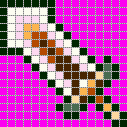
\includegraphics{video/sprite_1.png}
  \caption{Pattern Example}
\end{figure}

Using the default palette, which is initialised with RGB332 colours
from 0-255, the hexadecimal values for this pattern arranged in a
$16\times16$ array are shown below:

\begin{verbatim}
04040404040404E3E3E3E3E3E3E3E3E3
04FFFFFFFFFF04E3E3E3E3E3E3E3E3E3
04FFFBFBFBFF04E3E3E3E3E3E3E3E3E3
04FFFBF5F5FBFF04E3E3E3E3E3E3E3E3
04FFFBF5A8A8FBFF04E3E3E3E3E3E3E3
04FFFFFBA844A8FBFF04E3E3E3E3E3E3
040404FFFBA844A8FBFF04E3E3E3E3E3
E3E3E304FFFBA84444FBFF04E304E3E3
E3E3E3E304FFFB444444FBFF044D04E3
E3E3E3E3E304FFFB44444444FA4D04E3
E3E3E3E3E3E304FFFB44FFF54404E3E3
E3E3E3E3E3E3E304FF44F5A804E3E3E3
E3E3E3E3E3E3E3E304FA4404A804E3E3
E3E3E3E3E3E3E3044D4D04E304F504E3
E3E3E3E3E3E3E3E30404E3E3E304FA04
E3E3E3E3E3E3E3E3E3E3E3E3E3E30404

\end{verbatim}
Here \$E3 is used as the transparent index.

These 256 bytes would be stored in pattern memory in left to right,
top to bottom order.

\subparagraph{4-Bit Sprite Patterns}

The $16\times16$ pixel image uses 4-bits for each pixel so that each
pixel can be one of 16 colours. One colour indicates transparency and
this is programmed into the lower 4-bits of the Sprite Transparency
Index register (nextreg \$4B). By default the transparency value is
\$3. Note that the same register is shared with 8-bit patterns to
identify the transparent index.

Since each pixel only occupies 4-bits, two pixels are stored in each
byte. The leftmost pixel is stored in the upper 4-bits and the
rightmost pixel is stored in the lower 4-bits.

As an example we will use the same sprite image as was given in the
8-bit pattern example. Here only the lower 4 bits of each pixel is
retained to confine each pixel’s color to 4-bits:

\begin{verbatim}
4444444333333333
4FFFFF4333333333
4FBBBF4333333333
4FB55BF433333333
4FB588BF43333333
4FFB848BF4333333
444FB848BF433333
3334FB844BF43433
33334FB444BF4D43
333334FB4444AD43
3333334FB4F54433
33333334F4584333
333333334A448433
33333334DD434543
33333333443334A4
3333333333333344
\end{verbatim}

\$3 is used as the transparent index.

These 128 bytes would be stored in pattern memory in left to right,
top to bottom order.

The actual colour that will appear on screen will depend on the
palette, described below. The default palette will not likely generate
suitable colours for 4-bit sprites.

\subsection{Sprite Palette}
Each pixel of a sprite image is 8-bit for 8-bit patterns or 4-bit for
4-bit patterns. The pixel value is known as a pixel colour index. This
colour index is combined with the sprite’s palette offset. The palette
offset is a 4-bit value added to the top 4-bits of the pixel colour
index. The purpose of the palette offset is to allow a sprite to
change the colour of an image.

The final sprite colour index generated by the sprite hardware is then
the sum of the pixel index and the 4-bit palette offset. In pictures
using binary math:

\begin{verbatim}
8-bit Sprite
PPPP0000
+ IIIIIIII
----------
SSSSSSSS

4-bit Sprite
PPPP0000
+ 0000IIII
----------
SSSSSSSS = PPPPIIII
\end{verbatim}

Where “PPPP” is the 4-bit palette offset from the sprite’s attributes
and the “I”s represent the pixel value from the sprite pattern. The
final sprite index is represented by the 8-bit value “SSSSSSSS”.

For 4-bit sprites the palette offset can be thought of as selecting
one of 16 different 16-colour palettes.

This final 8-bit sprite index is then passed through the sprite
palette which acts like a lookup table that returns the 9-bit RGB333
colour associated with the sprite index.

At power up, the sprite palette is initialized such that the sprite
index passes through unchanged and is therefore interpretted as an
RGB332 colour. The missing third blue bit is generated as the logical
OR of the two other blue bits. In short, for 8-bit sprites, the sprite
index also acts like the colour when using the default palette.

\subsection{Sprite Attributes}
A sprite’s attributes is a list of properties that determine how and
where the sprite is drawn.

Each sprite is described by either 4 or 5 attribute bytes listed
below:

Sprite Attribute 0
\begin{verbatim}
X X X X X X X X
\end{verbatim}
The least significant eight bits of the sprite’s X coordinate. The
ninth bit is found in sprite attribute 2.

Sprite Attribute 1
\begin{verbatim}
Y Y Y Y Y Y Y Y
\end{verbatim}
The least significant eight bits of the sprite’s Y coordinate. The
ninth bit is optional and is found in attribute 4.

Sprite Attribute 2
\begin{verbatim}
P P P P XM YM R X8/PR
\end{verbatim}
P = 4-bit Palette Offset

XM = 1 to mirror the sprite image horizontally

YM = 1 to mirror the sprite image vertically

R = 1 to rotate the sprite image 90 degrees clockwise

X8 = Ninth bit of the sprite’s X coordinate

PR = 1 to indicate P is relative to the anchor’s palette offset
(relative sprites only)

Rotation is applied before mirroring.

Relative sprites, described below, replace X8 with PR.

\begin{figure}\centering
  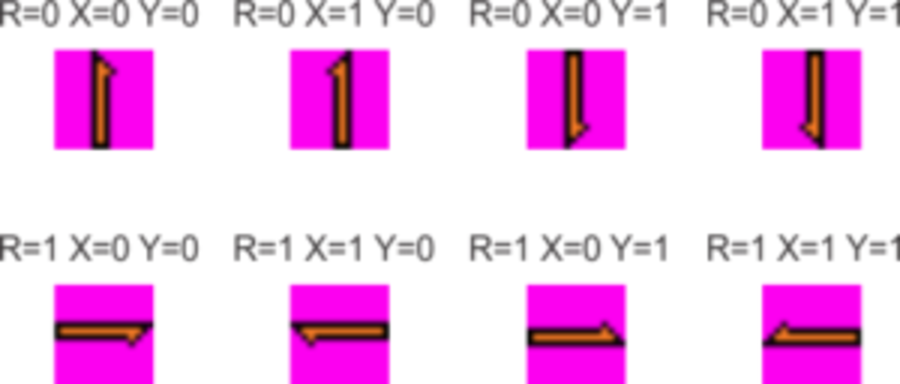
\includegraphics{video/flags.png}
  \caption{All Rotate and Mirror Flags}
\end{figure}

Sprite Attribute 3
\begin{verbatim}
V E N5 N4 N3 N2 N1 N0
\end{verbatim}
V = 1 to make the sprite visible

E = 1 to enable attribute byte 4

N = Sprite pattern to use 0-63

If E=0, the sprite is fully described by sprite attributes 0-3. The
sprite pattern is an 8-bit one identified by pattern N=0-63. The
sprite is an anchor and cannot be made relative. The sprite is
displayed as if sprite attribute 4 is zero.

If E=1, the sprite is further described by sprite attribute 4.

Sprite Attribute 4
\begin{enumerate}[A.]
\item Extended Anchor Sprite
\begin{verbatim}
H N6 T X X Y Y Y8
\end{verbatim}
H = 1 if the sprite pattern is 4-bit

N6 = 7th pattern bit if the sprite pattern is 4-bit

T = 0 if relative sprites are composite type else 1 for unified type

XX = Magnification in the X direction (00 = $1\times$, 01 = $2\times$,
10 = $4\times4$, 11 = $8\times$)

YY = Magnification in the Y direction (00 = $1\times$, 01 = $2\times$,
10 = $4\times$, 11 = $8\times$)

Y8 = Ninth bit of the sprite’s Y coordinate

{H,N6} must not equal {0,1} as this combination is used to indicate a
relative sprite.

\item Relative Sprite, Composite Type
\begin{verbatim}
0 1 N6 X X Y Y PO
\end{verbatim}
N6 = 7th pattern bit if the sprite pattern is 4-bit

XX = Magnification in the X direction (00 = $1\times$, 01 = $2\times$,
10 = $4\times$, 11 = $8\times$)

YY = Magnification in the Y direction (00 = $1\times$, 01 = $2\times$,
10 = $4\times$, 11 = $8\times$)

PO = 1 to indicate the sprite pattern number is relative to the
anchor’s

\item Relative Sprite, Unified Type
\begin{verbatim}
0 1 N6 0 0 0 0 PO
\end{verbatim}
N6 = 7th pattern bit if the sprite pattern is 4-bit

PO = 1 to indicate the sprite pattern number is relative to the
anchor’s
\end{enumerate}
The display surface for sprites is $320\times256$. The X coordinate of
the sprite is nine bits, ranging over 0-511, and the Y coordinate is
optionally nine bits again ranging over 0-511 or is eight bits ranging
over 0-255. The full extent 0-511 wraps on both axes, meaning a sprite
16 pixels wide plotted at X coordinate 511 would see its first pixel
not displayed (coordinate 511) and the following pixels displayed in
coordinates 0-14.

The full display area is visible in VGA. However, the HDMI display is
vertically shorter so the top eight pixel rows (Y = 0-7) and the
bottom eight pixel rows (Y = 248-255) will not be visible on an HDMI
display.

Sprites can be fully described by sprite attributes 0-3 if the E bit
in sprite attribute 3 is zero. These sprites are compatible with the
original sprite module from core versions prior to 2.00.26.

If the E bit is set then a fifth sprite attribute, sprite attribute 4,
becomes active. This attribute introduces scaling, 4-bit patterns, and
relative sprites. Scaling is self-explanatory and 4-bit patterns were
described in the last section. Relative sprites are described in the
next section.

\subsection{Relative Sprites}
Normal sprites (sprites that are not relative) are known as anchor
sprites. As the sprite module draws sprites in the order 0-127 (there
are 128 sprites), it internally stores characteristics of the last
anchor sprite seen. If following sprites are relative, they inherit
some of these characteristics, which allows relative sprites to have,
among other things, coordinates relative to the anchor. This means
moving the anchor sprite also causes its relatives to move with it.

There are two types of relative sprites supported known as “Composite
Sprites” and “Unified Sprites”. The type is determined by the anchor
in the T bit of sprite attribute 4.

\begin{enumerate}[A.]
\item Composite Sprites

  The sprite module records the following information from the anchor:
  \begin{itemize}
  \item Anchor.visible
  \item Anchor.Y
  \item Anchor.palette\_offset
  \item Anchor.N (pattern number)
  \item Anchor.H (indicates if the sprite uses 4-bit patterns)
  \end{itemize}
  These recorded items are not used by composite sprites:
  \begin{itemize}
  \item Anchor.rotate
  \item Anchor.xmirror
  \item Anchor.ymirror
  \item Anchor.xscale
  \item Anchor.yscale
  \end{itemize}
  The anchor determines if all its relative sprites use 4-bit patterns or not.
  
  The visibility of a particular relative sprite is the result of
  ANDing the anchor’s visibility with the relative sprite’s
  visibility. In other words, if the anchor is invisible then so are
  all its relatives.

  Relative sprites only have 8-bit X and Y coordinates (the ninth bits
  are taken for other purposes). These are signed offsets from the
  anchor’s X,Y coordinate. Moving the anchor moves all its relatives
  along with it.

  If the relative sprite has its PR bit set in sprite attribute 2,
  then the anchor’s palette offset is added to the relative sprite’s
  to determine the active palette offset for the relative
  sprite. Otherwise the relative sprite uses its own palette offset as
  usual.

  If the relative sprite has its PO bit set in sprite attribute 4,
  then the anchor’s pattern number is added to the relative sprite’s
  to determine the pattern used for display. Otherwise the relative
  sprite uses its own pattern number as usual. The intention is to
  supply a method to easily animate a large sprite by manipulating the
  pattern number in the anchor.

  A composite sprite is like a collection of independent sprites tied
  to an anchor.

\item Unified Sprites

  Unified sprites are a further extension of the
  composite type. The same information is recorded from the anchor and
  the same behaviour as described under composite sprites applies.

  The difference is the collection of anchor and relatives is treated
  as if it were a single $16\times16$ sprite. The anchor’s rotation,
  mirror, and scaling bits apply to all its relatives. Rotating the
  anchor causes all the relatives to rotate around the
  anchor. Mirroring the anchor causes the relatives to mirror around
  the anchor. The sprite hardware will automatically adjust X,Y coords
  and rotation, scaling and mirror bits of all relatives according to
  settings in the anchor.

  Unified sprites should be defined as if all its parts are
  $16\times16$ in size with the anchor controlling the look of the
  whole.

  A unified sprite is like a big version of an individual $16\times16$
  sprite controlled by the anchor.
\end{enumerate}

\subsection{Programming Sprites}

Sprites are created via three io registers and a nextreg interface.

Port \$303B (W)
\begin{verbatim}
X S S S S S S S
N6 X N N N N N N
\end{verbatim}
A write to this port has two effects.

One is it selects one of 128 sprites for writing sprite attributes via
port \$57.

The other is it selects one of 128 4-bit patterns in pattern memory
for writing sprite patterns via port \$5B. The N6 bit shown is the
least significant in the 7-bit pattern number and should always be
zero when selecting one of 64 8-bit patterns indicated by N.

Port \$57 (W)

Once a sprite is selected via port \$303B, its attributes can be
written to this port one byte after another. Sprites can have either
four or five attribute bytes and the internal attribute pointer will
move onto the next sprite after those four or five attribute bytes are
written. This means you can select a sprite via port \$303B and write
attributes for as many sequential sprites as desired. The attribute
pointer will roll over from sprite 127 to sprite 0.

Port \$5B (W)

Once a pattern number is selected via port \$303B, the 256-byte or
128-byte pattern can be written to this port. The internal pattern
pointer auto-increments after each write so as many sequential
patterns as desired can be written. The internal pattern pointer will
roll over from pattern 127 to pattern 0 (4-bit patterns) or from
pattern 63 to pattern 0 (8-bit patterns) automatically.

Port \$303B (R)

\begin{verbatim}
0 0 0 0 0 0 M C
\end{verbatim}
M = 1 if the maximum number of sprites per line was exceeded

C = 1 if any two displayed sprites collide on screen

Reading this port automatically resets the M and C bits.

Besides the i/o interface, there is a nextreg interface to sprite
attributes. The nextreg interface allows the copper to manipulate
sprites and grants the program random access to a sprite’s individual
attribute bytes.

(R/W) \$34 (52) $\Rightarrow$ Sprite Number

If the sprite number is in lockstep with io port \$303B (nextreg \$09
bit 4 is set)
\begin{itemize}
\item[] bits 7 = Pattern address offset (Add 128 to pattern address)
\item[] bits 6-0 = Sprite number 0-127, Pattern number 0-63
\end{itemize}
Selects which sprite has its attributes connected to the following registers.

Effectively performs an out to port \$303B with the same value

Otherwise
\begin{itemize}
\item[] bit 7 = Ignored
\item[] bits 6-0 = Sprite number 0-127
\end{itemize}
Selects which sprite has its attributes connected to the following registers.

Bit 7 always reads back as zero.

This nextreg can operate in two modes.

If nextreg \$09 bit 4 is set, then this register is kept in lockstep
with i/o port \$303B. A write to this nextreg is equivalent to a write
to port \$303B and vice versa. In this mode, the i/o interface and
nextreg interface are exactly equivalent.

If nextreg \$09 bit 4 is reset, then the nextreg interface is
decoupled from i/o port \$303B. This nextreg is used to select a
particular sprite 0-127 and this is completely independent from the
sprite selected for the i/o interface. This independence allows the
copper, for example, to manipulate different sprites than the cpu
using the i/o interface.

(W) \$35 (53) $\Rightarrow$ Sprite Attribute 0

(W) \$75 (117) $\Rightarrow$ Sprite Attribute 0 with automatic post
increment of Sprite Number
\begin{itemize}
\item[] bits 7-0 = LSB of X coordinate
\end{itemize}
A write to nextreg \$75 also increases the selected sprite in nextreg
\$34.

(W) \$36 (54) $\Rightarrow$ Sprite Attribute 1

(W) \$76 (118) $\Rightarrow$ Sprite Attribute 1 with automatic post
increment of Sprite Number
\begin{itemize}
\item[] bits 7-0 = LSB of Y coordinate
\end{itemize}
A write to nextreg \$76 also increases the selected sprite in nextreg
\$34.

(W) \$37 (55) $\Rightarrow$ Sprite Attribute 2

(W) \$77 (119) $\Rightarrow$ Sprite Attribute 2 with automatic post
increment of Sprite Number
\begin{itemize}
\item[] bits 7-4 = Palette offset added to top 4 bits of sprite colour
  index
\item[] bit 3 = X mirror
\item[] bit 2 = Y mirror
\item[] bit 1 = Rotate
\item[] bit 0 = MSB of X coordinate
\end{itemize}
A write to nextreg \$77 also increases the selected sprite in nextreg
\$34.

(W) \$38 (56) $\Rightarrow$ Sprite Attribute 3

(W) \$78 (120) $\Rightarrow$ Sprite Attribute 3 with automatic post
increment of Sprite Number
\begin{itemize}
\item[] bit 7 = Visible flag (1 = displayed)
\item[] bit 6 = Extended attribute (1 = Sprite Attribute 4 is active)
\item[] bits 5-0 = Pattern used by sprite (0-63)
\end{itemize}
A write to nextreg \$78 also increases the selected sprite in nextreg
\$34.

(W) \$39 (57) $\Rightarrow$ Sprite Attribute 4

(W) \$79 (121) $\Rightarrow$ Sprite Attribute 4 with automatic post
increment of Sprite Number

4-bit Sprites
\begin{itemize}
\item[] bit 7 = H (1 = sprite uses 4-bit patterns)
\item[] bit 6 = N6 (0 = use the first 128 bytes of the pattern else
  use the last 128 bytes)
\item[] bit 5 = 1 if relative sprites are composite, 0 if relative
  sprites are unified Scaling
\item[] bits 4-3 = X scaling (00 = 1x, 01 = 2x, 10 = 4x, 11 = 8x)
\item[] bits 2-1 = Y scaling (00 = 1x, 01 = 2x, 10 = 4x, 11 = 8x)
\item[] bit 0 = MSB of Y coordinate
\end{itemize}
A relative mode is enabled if H,N6 = 01. The byte format for relative
sprites is described above.

A write to nextreg \$79 also increases the selected sprite in nextreg
\$34.

\subsection{Global Control of Sprites}

The following nextreg are also of interest for sprites.

(R/W) \$09 (09) $\Rightarrow$ Peripheral 4 setting:
\begin{itemize}
\item[] bit 7 = Mono setting for AY 2 (1 = mono, 0 default)
\item[] bit 6 = Mono setting for AY 1 (1 = mono, 0 default)
\item[] bit 5 = Mono setting for AY 0 (1 = mono, 0 default)
\item[] bit 4 = Sprite id lockstep (1 = Nextreg \$34 and IO Port
  \$303B are in lockstep, 0 default)
\item[] bit 3 = Disables Kempston port (\$DF) if set
\item[] bit 2 = Disables divMMC ports (\$E3, \$E7, \$EB) if set
\item[] bits 1-0 = scanlines (0 after a PoR or Hard-reset)
  \begin{itemize}
  \item[] 00 = scanlines off
  \item[] 01 = scanlines 75\%
  \item[] 10 = scanlines 50\%
  \item[] 11 = scanlines 25\%
  \end{itemize}
\end{itemize}

Bit 4 determines if the i/o interface and nextreg interface operate in lockstep.

(R/W) \$15 (21) $\Rightarrow$ Sprite and Layers system
\begin{itemize}
\item[] bit 7 = LoRes mode, $128\times96\times256$ colours (1 =
  enabled)
\item[] bit 6 = Sprite priority (1 = sprite 0 on top, 0 = sprite 127
  on top)
\item[] bit 5 = Enable sprite clipping in over border mode (1 =
  enabled)
\item[] bits 4-2 = set layers priorities:

Reset default is 000, sprites over the Layer 2, over the ULA graphics
\begin{itemize}
\item[] 000 – S L U
\item[] 001 – L S U
\item[] 010 – S U L
\item[] 011 – L U S
\item[] 100 – U S L
\item[] 101 – U L S
\item[] 110 – S(U+L) ULA and Layer 2 combined, colours clamped to 7
\item[] 111 – S(U+L-5) ULA and Layer 2 combined, colours clamped to
  [0,7]
\end{itemize}
\item[] bit 1 = Over border (1 = yes)(Back to 0 after a reset)
\item[] bit 0 = Sprites visible (1 = visible)(Back to 0 after a reset)
\end{itemize}

Bit 0 must be set for sprites to be visible.

Bit 1 set allows sprites to be visible in the border area. When this
bit is reset, sprites will not display outside the $256\times192$ area
of the ULA display.

Bit 5 set enables clipping when sprites are visible in the border
area. If reset, no clipping is applied and sprites will be visible in
the full $320\times256$ space.

The sprite module draws sprites in the order 0-127 in each
scanline. Bit 6 determines whether sprite 0 is topmost or sprite 127
is topmost.

Bits 4:2 determine layer priority and how sprites overlay or are
obscured by other layers.

(R/W) \$19 (25) $\Rightarrow$ Clip Window Sprites
\begin{itemize}
\item[] bits 7-0 = Cood. of the clip window
  \begin{itemize}
  \item[] 1st write – X1 position
  \item[] 2nd write – X2 position
  \item[] 3rd write – Y1 position
  \item[] 4rd write – Y2 position
  \end{itemize}
\end{itemize}
The values are 0,255,0,191 after a Reset

Reads do not advance the clip position

When the clip window is enabled for sprites in “over border” mode, the
X coords are internally doubled and the clip window origin is moved to
the sprite origin inside the border.

Sprites will only be visible inside the clipping window. When not in
over-border mode (bit 1 of nextreg \$15) the clipping window is given
in ULA screen coordinates with 0,0 correspoding to the top left corner
of the ULA screen. In over-border mode, the clipping window’s origin
is moved to the sprite coordinate origin 32 pixels to the left and 32
pixels above the ULA screen origin.

Regardless, sprite position is always in sprite coordinates with 32,32
corresponding to the top left corner of the ULA screen.

(W) \$1C (28) $\Rightarrow$ Clip Window control
\begin{itemize}
\item[] bits 7-4 = Reserved, must be 0
\item[] bit 3 – reset the tilemap clip index
\item[] bit 2 – reset the ULA/LoRes clip index.
\item[] bit 1 – reset the sprite clip index.
\item[] bit 0 – reset the Layer 2 clip index.
\end{itemize}

Can be used to reset nextreg \$19.

(R/W) \$43 (67) $\Rightarrow$ Palette Control
\begin{itemize}
\item[] bit 7 = ‘1’ to disable palette write auto-increment.
\item[] bits 6-4 = Select palette for reading or writing:
  \begin{itemize}
  \item[] 000 = ULA first palette
  \item[] 100 = ULA second palette
  \item[] 001 = Layer 2 first palette
  \item[] 101 = Layer 2 second palette
  \item[] 010 = Sprites first palette
  \item[] 110 = Sprites second palette
  \item[] 011 = Tilemap first palette
  \item[] 111 = Tilemap second palette
  \end{itemize}
\item[] bit 3 = Select Sprites palette (0 = first palette, 1 = second
  palette)
\item[] bit 2 = Select Layer 2 palette (0 = first palette, 1 = second
  palette)
\item[] bit 1 = Select ULA palette (0 = first palette, 1 = second
  palette)
\item[] bit 0 = Enabe ULANext mode if 1. (0 after a reset)
\end{itemize}

Sprites have two associated palettes which can be selected in this nextreg.

(R/W) \$40 (64) $\Rightarrow$ Palette Index
\begin{itemize}
\item[] bits 7-0 = Select the palette index to change the associated
  colour.
\end{itemize}
For the ULA only, INKs are mapped to indices 0-7, Bright INKS to
indices 8-15, PAPERs to indices 16-23 and Bright PAPERs to indices
24-31.

In ULANext mode, INKs come from a subset of indices 0-127 and PAPERs
come from a subset of indices 128-255. The number of active indices
depends on the number of attribute bits assigned to INK and PAPER out
of the attribute byte.  The ULA always takes border colour from paper.

Select the starting palette index if writing the sprite palette.

Palette values can be written in either 8-bit or 9-bit form:

(R/W) \$41 (65) $\Rightarrow$ Palette Value (8 bit colour)
\begin{itemize}
\item[] bits 7-0 = Colour for the palette index selected by the register \$40.
\end{itemize}
(Format is RRRGGGBB – the lower blue bit of the 9-bit colour will be a
logical OR of blue bits 1 and 0 of this 8-bit value.)

After the write, the palette index is auto-incremented to the next
index if the auto-increment is enabled at reg \$43. Reads do not
auto-increment.

(R/W) \$44 (68) $\Rightarrow$ Palette Value (9 bit colour)

Two consecutive writes are needed to write the 9 bit colour
\begin{itemize}
\item[] 1st write:
  \begin{itemize}
  \item[] bits 7-0 = RRRGGGBB
  \end{itemize}
\item[] 2nd write.
  If writing a L2 palette
  \begin{itemize}
  \item[] bit 7 = 1 for L2 priority colour, 0 for normal

    Priority colour will always be on top even on an SLU priority
    arrangement. If you need the exact same colour on priority and non
    priority locations you will need to program the same colour twice
    changing bit 7 to 0 for the second colour
  \item[] bits 6-1 = Reserved, must be 0
  \item[] bit 0 = lsb B
  \end{itemize}
  
  If writing another palette
  \begin{itemize}
  \item[] bits 7-1 = Reserved, must be 0
  \item[] bit 0 = lsb B
  \end{itemize}
\end{itemize}


After the two consecutives writes the palette index is
auto-incremented if the auto-increment is enabled by reg \$43.

Reads only return the 2nd byte and do not auto-increment.

(R/W) \$4B (75) $\Rightarrow$ Transparency index for sprites
\begin{itemize}
\item[] bits 7-0 = Set the index value (\$E3 after reset)
\end{itemize}
For 4-bit sprites only the bottom 4-bits are relevant.

Determines the transparent colour index used for sprites.


\section{Audio}
\subsection{Internal Speaker}

The baseline sound of the ZX Spectrum was produced by toggling the Ear
bit (bit 4) of \$fe (254) The ULA port to produce 1-bit audio.  It is
enabled by bit 4 of Next register \$08 (8).  While this does work on
the ZX Spectrum Next, there are other much better methods and this is
only supported for backward compatibility.

Code:
\begin{verbatim}
;; enable internal speaker
ld bc,$243B
ld a,$08
out (c),a
ld bc,$253B
in a,(c)
or $10
out (c),a
\end{verbatim}

\subsection{Spectdrum/Convox}

This is 8-bit D/A audio.  It is enabled by setting bit 3 of Next
register \$08 (8).  After that audio can be controlled by writing
linear 8-bit unsigned values to port \$df (223).

Code:
\begin{verbatim}
;; enable SpecDrum/Convox audio
ld bc,$243B
ld a,$08
out (c),a
ld bc,$253B
in a,(c)
or $08
out (c),a
\end{verbatim}

\subsection{Turbosound}

TurboSound consists of the implementation of three AY-3-8912 chips. To
enable TurboSound set bit 1 of Next Register \$08 (8). Once enabled
the sound chips and registers of the sound chips are selected using
port \$fffd (65533) TurboSound Next Control while the registers are
accessed using \$bffd () Sound Chip Register Access.  To enable access
to a particular chip write 111111xx to the control register where
01=AY1, 10=AY2, and 11=AY3.  Access to particular registers of the
selected chip is selected by writing the register number to the
control register. You can then access a chip register using the access
port.

Code:
\begin{verbatim}
;; enable TurboSound audio
ld bc,$243B
ld a,$08
out (c),a
ld bc,$253B
in a,(c)
or $02
out (c),a
\end{verbatim}

Each of the three AY chips has three channels, A, B, and C whose
mapping is controlled by bit 5 of Next register 0x08 (8).

\begin{itemize}
\item (R/W) 0x00 (0) $\Rightarrow$ Channel A fine tune
\item (R/W) 0x01 (1) $\Rightarrow$ Channel A coarse tune (4 bits)
\item (R/W) 0x02 (2) $\Rightarrow$ Channel B fine tune
\item (R/W) 0x03 (3) $\Rightarrow$ Channel B coarse tune (4 bits)
\item (R/W) 0x04 (4) $\Rightarrow$ Channel C fine tune
\item (R/W) 0x05 (5) $\Rightarrow$ Channel C coarse tune (4 bits)
\item (R/W) 0x06 (6) $\Rightarrow$ Noise period (5 bits)
\item (R/W) 0x07 (7) $\Rightarrow$ Tone Enable
  \begin{itemize}
  \item bit 5: Channel C tone enable (0=enable, 1=disable)
  \item bit 4: Channel B tone enable (0=enable, 1=disable)
  \item bit 3: Channel A tone enable (0=enable, 1=disable)
  \item bit 2: Channel C noise enable (0=enable, 1=disable)
  \item bit 1: Channel B noise enable (0=enable, 1=disable)
  \item bit 0: Channel A noise enable (0=enable, 1=disable)
  \end{itemize}
\item (R/W) 0x08 (8) $\Rightarrow$ Channel A amplitude
  \begin{itemize}
  \item bit 4: 0=fixed amplitude, 1=use envelope generator (bits 0-3 ignored)
  \item bits 0-3: value of fixed amplitude
  \end{itemize}
\item (R/W) 0x09 (9) $\Rightarrow$ Channel B amplitude
  \begin{itemize}
  \item bit 4: 0=fixed amplitude, 1=use envelope generator (bits 0-3 ignored)
  \item bits 0-3: value of fixed amplitude
  \end{itemize}
\item (R/W) 0x0A (10) $\Rightarrow$ Channel C amplitude
  \begin{itemize}
  \item bit 4: 0=fixed amplitude, 1=use envelope generator (bits 0-3 ignored)
  \item bits 0-3: value of fixed amplitude
  \end{itemize}
\item (R/W) 0x0B (11) $\Rightarrow$ Envelope period fine
\item (R/W) 0x0C (12) $\Rightarrow$ Envelope period coarse
\item (R/W) 0x0D (13) $\Rightarrow$ Envelope shape
  \begin{itemize}
  \item bit 3: Continue: 0=drop to amplitude 0 after 1 cycle, 1=use ‘Hold’ value
  \item bit 2: Attack: 0=generator counts down, 1=generator counts up
  \item bit 1: Alternate:
    \begin{itemize}
    \item hold=0: 0=generator resets after each cycle, 1=generator
      reverses direction each cycle
    \item hold=1: 0=hold final value, 1=hold initial value
    \end{itemize}
  \item bit 0: Hold: 0=cycle continuously, 1=perform one cycle and hold
  \end{itemize}
\end{itemize}


% This file was converted from HTML to LaTeX with
% gnuhtml2latex program
% (c) Tomasz Wegrzanowski <maniek@beer.com> 1999
% (c) Gunnar Wolf <gwolf@gwolf.org> 2005-2010
% Version : 0.4.
\documentclass{article}
\begin{document}
\section*{TSconf: Memory}

Development

\textbf{Consider the memory location in the system. }

ZX Evolution has 4MB of memory.

The organization of this memory is similar to zx spectrum 128 - paging
is used.

Transcribed into pages of memory, we have 256 pages of 16 kb each.

The above picture describes how the memory of the Spectrum is
organized. A similar system is used in TSconf, but somewhat expanded -
we are able to place pages not only from the address \#c000:

\begin{verbatim}
    Page0 (port #10af) - адрес #0000
    Page1 (port #11af) - адрес #4000
    Page2 (port #12af) - адрес #8000
    Page3 (port #13af) - адрес #c000
\end{verbatim}

Writing to the port switches the page in the window we need.

To use the paging system from address \#0000, you need to use the
MemConfig port (\#21af):

\begin{quotation}
  \textbf{Port MemConfig, \#21af:}

  MemConfig LCK128 [1: 0] - - W0\_RAM! W0\_MAP W0\_WE ROM128

  bits 7.6 - LCK128 - memory mode: 00-512k, 01 - 128k, 10 - Auto, 11 -
  1024 k. The default is data from the BIOS.

  bit 3 - W0\_RAM, 2 - W0\_MAP, 1 - W0\_WE, bit 0 - ROM128 (the same
  as bit 4 in \#7FFD)

  W0\_RAM 0 - ROM / 1 - RAM

  ! W0\_MAP 0 - mapped / 1 - Page0

  W0\_WE 0 - WP / 1 - WE (for ROM and RAM)
\end{quotation}
With its help, it is possible to switch the 0th memory window to read
/ write mode (the usual state is read only, there is the specter ROM),
and to enable mapping - the ability to place other pages of memory,
not just the standard page 0.

In window \#0000 you can enable RAM instead of ROM with optional
prohibition of recording in this window.

W0\_RAM = 0 - enabled ROM

W0\_RAM = 1 - enabled RAM

Bit W0\_WE allows writing for RAM and programming (WE signal for ROM):

W0\_WE = 0

W0\_RAM = 0 - ROM firmware is disabled

W0\_RAM = 1 - writing to RAM at \#0000-3FFF not allowed

W0\_WE = 1

W0\_RAM = 0 - ROM firmware is allowed

W0\_RAM = 1 - writing to RAM at \#0000-3FFF is allowed

\textbf{Bit W0\_MAP}sets the page selection method for window \#0000.

W0\_MAP = 0 - the page number is selected depending on the current ZX
mode (Basic 48, Basic 128, TR-DOS).

Page layout: 0 - system, 1 - TR-DOS, 2 - Basic 128, 3 - Basic 48.

However, the register Page0 selects a bank of 4 pages to be used:

W0\_RAM = 0 - for window \#0000 is selected ROM

Page0 = 0bxxx000xx - pages 0-3 are used,

Page0 = 0bxxx001xx - pages 4-7 are used,

...

Page0 = 0bxxx111xx - pages 28-31 are used.

W0\_RAM = 1 - RAM is selected for the window \#0000 - this mode can be
used to debug the firmware without reprogramming the ROM or testing
non-standard pzushek.

Page0 = 0b000000xx - pages 0-3 are used,

Page0 = 0b000001xx - pages 4-7 are used,

...

Page0 = 0b111111xx - pages 252-255 are used.

W0\_MAP = 1 - the page number is taken directly from the register
Page0 - linear mode

W0\_RAM = 0 - pages

0-31 ROM W0\_RAM = 1 - pages 0-255 RAM

\textbf{Example:}

Turn on page \#80 from address \#8000

\begin{verbatim}
		ld a,#80
		ld bc,PAGE2
		out (c),a
\end{verbatim}

Enable the ability to work in page 0

\begin{verbatim}
		ld bc,MemConfig
		ld a,%00001110
		out (c),a
\end{verbatim}

Voila, write, post with 0000.

\subsubsection*{2 comments}

Does this only concern tsconf or the whole evo as a whole?

Only tskonf. The architecture of the Eva is mostly due to the
configuration in the FPSA.

\end{document}

\chapter{zxnDMA}
 February 25, 2019  Phoebus Dokos  Off  Hardware, Resources,

The ZX Spectrum Next DMA (zxnDMA)

\section{Overview}

The ZX Spectrum Next DMA (zxnDMA) is a single channel dma device that
implements a subset of the Z80 DMA functionality. The subset is large
enough to be compatible with common uses of the similar Datagear
interface available for standard ZX Spectrum computers and
compatibles. It also adds a burst mode capability that can deliver
audio at programmable sample rates to the DAC device.

\section{Accessing the zxnDMA}
The zxnDMA is mapped to a single Read/Write IO Port 0x6B which is the
same one used by the Datagear but unlike the Datagear it doesn't also
map itself to a second port 0x0B similar to the MB-02 interface.

\begin{verbatim}
PORT $6b: zxnDMA
\end{verbatim}

\section{Description}
The normal Z80 DMA (Z8410) chip is a pipelined device and because of
that it has numerous off-by-one idiosyncrasies and requirements on the
order that certain commands should be carried out. These issues are
not duplicated in the zxnDMA. You can continue to program the zxnDMA
as if it is were a Z8410 DMA device but it can also be programmed in a
simpler manner.

The single channel of the zxnDMA chip consists of two ports named A
and B. Transfers can occur in either direction between ports A and B,
each port can describe a target in memory or IO, and each can be
configured to autoincrement, autodecrement or stay fixed after a byte
is transferred.

A special feature of the zxnDMA can force each byte transfer to take a
fixed amount of time so that the zxnDMA can be used to deliver sampled
audio.

\section{Modes of Operation}
The zxnDMA can operate in a z80-dma compatibility mode.

The z80-dma compatibility mode is selected by setting bit 6 of nextreg
\$06. In this mode, all transfers involve length+1 bytes which is the
same behaviour as the z80-dma chip. In zxn-dma mode, the transfer
length is exactly the number of bytes programmed. This mode is mainly
present to accommodate existing spectrum software that uses the
z80-dma and for cp/m programs that may have a z80-dma option.

The zxnDMA can also operate in either burst or continuous modes.

Continuous mode means the DMA chip runs to completion without allowing
the CPU to run. When the CPU starts the DMA, the DMA operation will
complete before the CPU executes its next instruction.

Burst mode nominally means the DMA lets the CPU run if either port is
not ready. This condition can't happen in the zxnDMA chip except when
operated in the special fixed time transfer mode. In this mode, the
zxnDMA will let the CPU run while it waits for the fixed time to
expire between bytes transferred.

Note that there is no byte transfer mode as in the Z80 DMA.

\section{Programming the zxnDMA}
Like the Z80 DMA chip, the zxnDMA has seven write registers named
WR0-WR6 that control the device. Each register WR0-WR6 can have zero
or more parameters associated with it.

In a first write to the zxnDMA port, the write value is compared
against a bitmask to determine which of the WR0-WR6 is the
target. Remaining bits in the written value can contain data as well
as a list of associated parameter bits. The parameter bits determine
if further writes are expected to deliver parameter values. If there
are multiple parameter bits set, the expected order of parameter
values written is determined by parameter bit position from right to
left (bit 0 through bit 7). Once all parameters are written, the
zxnDMA again expects a regular register write selecting WR0-WR6.

The table X.Y describes the registers and the bitmask required to
select them on the zxnDMA.

\begin{table}[h]\centering
  \caption{zxnDMA Registers}
  \csvautotabular{zxndma/registers.csv}
\end{table}

\section{zxnDMA Registers}
These are described below following the same convention used by Zilog
for its DMA chip:

\paragraph{WR0 – Write Register Group 0}
\begin{verbatim}
D7  D6  D5  D4  D3  D2  D1  D0  BASE REGISTER BYTE
 0   |   |   |   |   |   |   |
     |   |   |   |   |   0   0  Do not use
     |   |   |   |   |   0   1  Transfer (Prefer this for Z80 DMA compatibility)
     |   |   |   |   |   1   0  Do not use (Behaves like Transfer, Search on Z80
     |   |   |   |   |                       DMA)
     |   |   |   |   |   1   1  Do not use (Behaves like Transfer, Search/Trans-
     |   |   |   |   |                      fer on Z80 DMA)
     |   |   |   |   0 = Port B -> Port A (Byte transfer direction)
     |   |   |   |   1 = Port A -> Port B
     |   |   |   V
D7  D6  D5  D4  D3  D2  D1  D0  PORT A STARTING ADDRESS (LOW BYTE)
     |   |   V
D7  D6  D5  D4  D3  D2  D1  D0  PORT A STARTING ADDRESS (HIGH BYTE)
     |   V
D7  D6  D5  D4  D3  D2  D1  D0  BLOCK LENGTH (LOW BYTE)
     V
D7  D6  D5  D4  D3  D2  D1  D0  BLOCK LENGTH (HIGH BYTE)
\end{verbatim}
Several registers are accessible from WR0. The first write to WR0 is
to the base register byte. Bits D6:D3 are optionally set to indicate
that associated registers in this group will be written next. The
order the writes come in are from D3 to D6 (right to left). For
example, if bits D6 and D3 are set, the next two writes will be
directed to PORT A STARTING ADDRESS LOW followed by BLOCK LENGTH HIGH.

\paragraph{WR1 – Write Register Group 1}
\begin{verbatim}
D7  D6  D5  D4  D3  D2  D1  D0  BASE REGISTER BYTE
 0   |   |   |   |   1   0   0
     |   |   |   |
     |   |   |   0 = Port A is memory
     |   |   |   1 = Port A is IO
     |   |   |
     |   0   0 = Port A address decrements
     |   0   1 = Port A address increments
     |   1   0 = Port A address is fixed
     |   1   1 = Port A address is fixed
     |
     V
D7  D6  D5  D4  D3  D2  D1  D0  PORT A VARIABLE TIMING BYTE
 0   0   0   0   0   0   |   |
                         0   0 = Cycle Length = 4
                         0   1 = Cycle Length = 3
                         1   0 = Cycle Length = 2
                         1   1 = Do not use
\end{verbatim}
The cycle length is the number of cycles used in a read or write
 operation. The first cycle asserts signals and the last cycle
 releases them. There is no half cycle timing for the control signals.

\paragraph{WR2 – Write Register Group 2}
\begin{verbatim}
D7  D6  D5  D4  D3  D2  D1  D0  BASE REGISTER BYTE
 0   |   |   |   |   0   0   0
     |   |   |   |
     |   |   |   0 = Port B is memory
     |   |   |   1 = Port B is IO
     |   |   |
     |   0   0 = Port B address decrements
     |   0   1 = Port B address increments
     |   1   0 = Port B address is fixed
     |   1   1 = Port B address is fixed
     |
     V
D7  D6  D5  D4  D3  D2  D1  D0  PORT B VARIABLE TIMING BYTE
 0   0   |   0   0   0   |   |
         |               0   0 = Cycle Length = 4
         |               0   1 = Cycle Length = 3
         |               1   0 = Cycle Length = 2
         |               1   1 = Do not use
         |
         V
D7  D6  D5  D4  D3  D2  D1  D0  ZXN PRESCALAR (FIXED TIME TRANSFER)
\end{verbatim}
The ZXN PRESCALAR is a feature of the zxnDMA implementation. If
non-zero, a delay will be inserted after each byte is transferred such
that the total time needed for each transfer is determined by the
prescalar. This works in both the continuous mode and the burst
mode. If the DMA is operated in burst mode, the DMA will give up any
waiting time to the CPU so that the CPU can run while the DMA is idle.

The rate of transfer is given by the formula "Frate = 875kHz /
prescalar" or, rearranged, "prescalar = 875kHz / Frate". The formula
is framed in terms of a sample rate (Frate) but Frate can be inverted
to set a transfer time for each byte instead. The 875kHz constant is a
nominal value assuming a 28MHz system clock; the system clock actually
varies from this depending on the video timing selected by the user
(HDMI, VGA0-6) so for complete accuracy the constant should be
prorated according to documentation for nextreg \$11.

In a DMA audio setting, selecting a sample rate of 16kHz would mean
setting the prescalar value to 55. This sample period is constant
across changes in CPU speed.

\paragraph{WR3 – Write Register Group 3}
\begin{verbatim}
D7  D6  D5  D4  D3  D2  D1  D0  BASE REGISTER BYTE
 1   |   0   0   0   0   0   0
     |
     1 = DMA Enable
\end{verbatim}
The Z80 DMA defines more fields but they are ignored by the zxnDMA.

The two other registers defined by the Z80 DMA in this group on D4 and
D3 are implemented by the zxnDMA but they do nothing.

It is preferred to start the DMA by writing an Enable DMA command to
WR6.

\paragraph{WR4 – Write Register Group 4}
\begin{verbatim}
D7  D6  D5  D4  D3  D2  D1  D0  BASE REGISTER BYTE
 1   |   |   0   |   |   0   1
     |   |       |   |
     0   0 = Do not use (Behaves like Continuous mode, Byte mode on Z80 DMA)
     0   1 = Continuous mode
     1   0 = Burst mode
     1   1 = Do not use
                 |   |
                 |   V
D7  D6  D5  D4  D3  D2  D1  D0  PORT B STARTING ADDRESS (LOW BYTE)
                 |
                 V
D7  D6  D5  D4  D3  D2  D1  D0  PORT B STARTING ADDRESS (HIGH BYTE)
\end{verbatim}
The Z80 DMA defines three more registers in this group through D4 that
define interrupt behaviour. Interrups and pulse generation are not
implemented in the zxnDMA nor are these registers available for
writing.

\paragraph{WR5 – Write Register Group 5}
\begin{verbatim}
D7  D6  D5  D4  D3  D2  D1  D0  BASE REGISTER BYTE
 1   0   |   |   0   0   1   0
         |   |
         |   0 = /ce only
         |   1 = /ce & /wait multiplexed
         |
         0 = Stop on end of block
         1 = Auto restart on end of block
\end{verbatim}
The /ce \& /wait mode is implemented in the zxnDMA but is not currently
used. This mode has an external device using the DMA's /ce pin to
insert wait states during the DMA's transfer.

The auto restart feature causes the DMA to automatically reload its
source and destination addresses and reset its byte counter to zero to
repeat the last transfer when a previous one is finished.

\paragraph{WR6 – Command Register}
\begin{verbatim}
D7  D6  D5  D4  D3  D2  D1  D0  BASE REGISTER BYTE
 1   ?   ?   ?   ?   ?   1   1
     |   |   |   |   |
     1   0   0   0   0 = \$C3 = Reset
     1   0   0   0   1 = \$C7 = Reset Port A Timing
     1   0   0   1   0 = \$CB = Reset Port B Timing
     0   1   1   1   1 = \$BF = Read Status Byte
     0   0   0   1   0 = \$8B = Reinitialize Status Byte
     0   1   0   0   1 = \$A7 = Initialize Read Sequence
     1   0   0   1   1 = \$CF = Load
     1   0   1   0   0 = \$D3 = Continue
     0   0   0   0   1 = \$87 = Enable DMA
     0   0   0   0   0 = \$83 = Disable DMA
 +-- 0   1   1   1   0 = \$BB = Read Mask Follows
 |
D7  D6  D5  D4  D3  D2  D1  D0  READ MASK
 0   |   |   |   |   |   |   |
     |   |   |   |   |   |   V
D7  D6  D5  D4  D3  D2  D1  D0  Status Byte
     |   |   |   |   |   |
     |   |   |   |   |   V
D7  D6  D5  D4  D3  D2  D1  D0  Byte Counter Low
     |   |   |   |   |
     |   |   |   |   V
D7  D6  D5  D4  D3  D2  D1  D0  Byte Counter High
     |   |   |   |
     |   |   |   V
D7  D6  D5  D4  D3  D2  D1  D0  Port A Address Low
     |   |   |
     |   |   V
D7  D6  D5  D4  D3  D2  D1  D0  Port A Address High
     |   |
     |   V
D7  D6  D5  D4  D3  D2  D1  D0  Port B Address Low
     |
     V
D7  D6  D5  D4  D3  D2  D1  D0  Port B Address High
\end{verbatim}
Unimplemented Z80 DMA commands are ignored.

Prior to starting the DMA, a LOAD command must be issued to copy the
Port A and Port B addresses into the DMA's internal pointers. Then an
ìEnable DMAî command is issued to start the DMA.

The ìContinueî command resets the DMA’s byte counter so that a
following ìEnable DMAî allows the DMA to repeat the last transfer but
using the current internal address pointers. I.e. it continues from
where the last copy operation left off.

Registers can be read via an IO read from the DMA port after setting
the read mask. (At power up the read mask is set to \$7f). Register
values are the current internal dma counter values. So ìPort Address A
Lowî is the lower 8-bits of Port A’s next transfer address. Once the
end of the read mask is reached, further reads loop around to the
first one.

The format of the DMA status byte is as follows:

00E1101T

E is set to 0 if the total block length has been transferred
at least once.

T is set to 1 if at least one byte has been transferred.

\paragraph{Operating speed}

The zxnDMA operates at the same speed as the CPU, that is 3.5MHz, 7MHz
or 14MHz. This is a contended clock that is modified by the ULA and
the auto-slowdown by Layer2.

Auto-slowdown occurs without user intervention if speed exceeds 7Mhz
and the active Layer2 display is being generated (higher speed
operation resumes when the active Layer2 display is not
generated). Programmers do NOT need to account for speed differences
regarding DMA transfers as this happens automatically.

Because of this, the cycle lengths for Ports A and B can be set to
their minimum values without ill effects. The cycle lengths specified
for Ports A and B are intended to selectively slow down read or write
cycles for hardware that cannot operate at the DMA's full speed.

\paragraph{The DMA and Interrupts}

The zxnDMA cannot currently generate interrupts.

The other side of this is that while the DMA controls the bus, the Z80
cannot respond to interrupts. On the Z80, the nmi interrupt is edge
triggered so if an nmi occurs the fact that it occurred is stored
internally in the Z80 so that it will respond when it is woken up. On
the other hand, maskable interrupts are level triggered. That is, the
Z80 must be active to regularly sample the /INT line to determine if a
maskable interrupt is occurring. On the Spectrum and the ZX Next, the
ULA (and line interrupt) are only asserted for a fixed amount of time
~30 cycles at 3.5MHz. If the DMA is executing a transfer while the
interrupt is asserted, the CPU will not be able to see this and it
will most likely miss the interrupt. In burst mode, the CPU will never
miss these interrupts, although this may change if multiple channels
are implemented.

\section{Programming examples}

A simple way to program the DMA is to walk down the list of registers
WR0-WR5, sending desired settings to each. Then start the DMA by
sending a LOAD command followed by an ENABLE\_DMA command to WR6. Once
more familiar with the DMA, you will discover that the amount of
information sent can be reduced to what changes between transfers.

\begin{enumerate}
\item Assembly

  Short example program to DMA memory to the screen then DMA a sprite
  image from memory to sprite RAM, and then showing said sprite scroll
  across the screen.
\begin{verbatim}
;------------------------------------------------------------------------------
device zxspectrum48
;------------------------------------------------------------------------------
; DEFINE testing
;------------------------------------------------------------------------------
; DMA (Register 6)
;
;------------------------------------------------------------------------------
;zxnDMA programming example
;------------------------------------------------------------------------------
;(c) Jim Bagley
;------------------------------------------------------------------------------
DMA_RESET equ $c3
DMA_RESET_PORT_A_TIMING equ $c7
DMA_RESET_PORT_B_TIMING equ $cb
DMA_LOAD equ $cf ; %11001111
DMA_CONTINUE equ $d3
DMA_DISABLE_INTERUPTS equ $af
DMA_ENABLE_INTERUPTS equ $ab
DMA_RESET_DISABLE_INTERUPTS equ $a3
DMA_ENABLE_AFTER_RETI equ $b7
DMA_READ_STATUS_BYTE equ $bf
DMA_REINIT_STATUS_BYTE equ $8b
DMA_START_READ_SEQUENCE equ $a7
DMA_FORCE_READY equ $b3
DMA_DISABLE equ $83
DMA_ENABLE equ $87
DMA_WRITE_REGISTER_COMMAND equ $bb
DMA_BURST equ %11001101
DMA_CONTINUOUS equ %10101101
ZXN_DMA_PORT equ $6b
SPRITE_STATUS_SLOT_SELECT equ $303B
SPRITE_IMAGE_PORT equ $5b
SPRITE_INFO_PORT equ $57
;------------------------------------------------------------------------------

IFDEF testing
org $6000
ELSE
org $2000
ENDIF

start
ld hl,$0000
ld de,$4000
ld bc,$800
call TransferDMA ; copy some random data to the screen pointing
; to ROM for now, for the purpose of showing
; how to do a DMA copy.
ld a,0 ; sprite image number we want to update
ld bc,SPRITE_STATUS_SLOT_SELECT
out (c),a ; set the sprite image number
ld bc,1*256 ; number to transfer (1)
ld hl,testsprite ; from
call TransferDMASprite ; transfer to sprite ram

nextreg 21,1 ; turn sprite on. for more info on this check
; out https://www.specnext.com/tbblue-io-port-system/
ld de,0
ld (xpos),de ; set initial X position ( doesn't need it for
; this demo, but if you run the .loop again it
; will continue from where it was
ld a,$20
ld (ypos),a ; set initial Y position

.loop
ld a,0 ; sprite number we want to position
ld bc,SPRITE_STATUS_SLOT_SELECT
out (c),a
ld de,(xpos)
ld hl,(ypos) ; ignores H so doing this rather than
; ld a,(ypos):ld l,a
ld bc,(image) ; not flipped or palette shifted
call SetSprite

halt

ld de,(xpos)
inc de
ld (xpos),de
ld a,d
cp $01
jr nz,.loop ; if high byte of xpos is not 1 (right of
; screen )
ld a,e
cp $20+1
jr nz,.loop ; if low byte is not $21 just off the right of
; the screen, $20 is off screen but as the
; INC DE is just above and not updated sprite
; after it, it needs to be $21
xor a
ret ; return back to basic with OK

xpos dw 0 ; x position
ypos db 0 ; y position
; these next two BITS and IMAGE are swapped
; as bits needs to go into B register image
; db 0+$80 ; use image 0 (for the image we
; transfered)+$80 to set the sprite to active
bits db 0 ; not flipped or palette shifted

c1 = %11100000
c2 = %11000000
c3 = %10100000
c4 = %10000000
c5 = %01100000
c6 = %01000000
c7 = %00100000
c8 = %00000000

testsprite
db c1,c1,c1,c1,c1,c1,c1,c1,c1,c1,c1,c1,c1,c1,c1,c1
db c1,c2,c2,c2,c2,c2,c2,c2,c2,c2,c2,c2,c2,c2,c2,c1
db c1,c2,c3,c3,c3,c3,c3,c3,c3,c3,c3,c3,c3,c3,c2,c1
db c1,c2,c3,c4,c4,c4,c4,c4,c4,c4,c4,c4,c4,c3,c2,c1
db c1,c2,c3,c4,c5,c5,c5,c5,c5,c5,c5,c5,c4,c3,c2,c1
db c1,c2,c3,c4,c5,c6,c6,c6,c6,c6,c6,c5,c4,c3,c2,c1
db c1,c2,c3,c4,c5,c6,c7,c7,c7,c7,c6,c5,c4,c3,c2,c1
db c1,c2,c3,c4,c5,c6,c7,c8,c8,c7,c6,c5,c4,c3,c2,c1
db c1,c2,c3,c4,c5,c6,c7,c8,c8,c7,c6,c5,c4,c3,c2,c1
db c1,c2,c3,c4,c5,c6,c7,c7,c7,c7,c6,c5,c4,c3,c2,c1
db c1,c2,c3,c4,c5,c6,c6,c6,c6,c6,c6,c5,c4,c3,c2,c1
db c1,c2,c3,c4,c5,c5,c5,c5,c5,c5,c5,c5,c4,c3,c2,c1
db c1,c2,c3,c4,c4,c4,c4,c4,c4,c4,c4,c4,c4,c3,c2,c1
db c1,c2,c3,c3,c3,c3,c3,c3,c3,c3,c3,c3,c3,c3,c2,c1
db c1,c2,c2,c2,c2,c2,c2,c2,c2,c2,c2,c2,c2,c2,c2,c1
db c1,c1,c1,c1,c1,c1,c1,c1,c1,c1,c1,c1,c1,c1,c1,c1

;-------------------------------------------------
; de = X
; l = Y
; b = bits
; c = sprite image
SetSprite
push bc
ld bc,SPRITE_INFO_PORT
out (c),e ; Xpos
out (c),l ; Ypos
pop hl
ld a,d
and 1
or h
out (c),a
ld a,l:or $80
out (c),a ; image
ret

;--------------------------------
; hl = source
; de = destination
; bc = length
;--------------------------------
TransferDMA
di
ld (DMASource),hl
ld (DMADest),de
ld (DMALength),bc
ld hl,DMACode
ld b,DMACode_Len
ld c,ZXN_DMA_PORT
otir
ei
ret

DMACode db DMA_DISABLE
db %01111101 ; R0-Transfer mode, A -> B, write adress
; + block length
DMASource dw 0 ; R0-Port A, Start address
; (source address)
DMALength dw 0 ; R0-Block length (length in bytes)
db %01010100 ; R1-write A time byte, increment, to
; memory, bitmask
db %00000010 ; 2t
db %01010000 ; R2-write B time byte, increment, to
; memory, bitmask
db %00000010 ; R2-Cycle length port B
db DMA_CONTINUOUS ; R4-Continuous mode (use this for block
; transfer), write dest adress
DMADest dw 0 ; R4-Dest address (destination address)
db %10000010 ; R5-Restart on end of block, RDY active
; LOW
db DMA_LOAD ; R6-Load
db DMA_ENABLE ; R6-Enable DMA

DMACode_Len equ $-DMACode

;------------------------------------------------------------------------------
; hl = source
; bc = length
; set port to write to with TBBLUE_REGISTER_SELECT
; prior to call
;------------------------------------------------------------------------------
TransferDMAPort
di
ld (DMASourceP),hl
ld (DMALengthP),bc
ld hl,DMACodeP
ld b,DMACode_LenP
ld c,ZXN_DMA_PORT
otir
ei
ret

DMACodeP db DMA_DISABLE
db %01111101 ; R0-Transfer mode, A -> B, write adress
; + block length
DMASourceP dw 0 ; R0-Port A, Start address (source address)
DMALengthP dw 0 ; R0-Block length (length in bytes)
db %01010100 ; R1-read A time byte, increment, to
; memory, bitmask
db %00000010 ; R1-Cycle length port A
db %01101000 ; R2-write B time byte, increment, to
; memory, bitmask
db %00000010 ; R2-Cycle length port B
db %10101101 ; R4-Continuous mode (use this for block
; transfer), write dest adress
dw $253b ; R4-Dest address (destination address)
db %10000010 ; R5-Restart on end of block, RDY active
; LOW
db DMA_LOAD ; R6-Load
db DMA_ENABLE ; R6-Enable DMA

DMACode_LenP equ $-DMACodeP
;------------------------------------------------------------------------------
; hl = source
; bc = length
;------------------------------------------------------------------------------
TransferDMASprite
di
ld (DMASourceS),hl
ld (DMALengthS),bc
ld hl,DMACodeS
ld b,DMACode_LenS
ld c,ZXN_DMA_PORT
otir
ei
ret

DMACodeS db DMA_DISABLE
db %01111101 ; R0-Transfer mode, A -> B, write adress
; + block length
DMASourceS dw 0 ; R0-Port A, Start address (source address)
DMALengthS dw 0 ; R0-Block length (length in bytes)
db %01010100 ; R1-read A time byte, increment, to
; memory, bitmask
db %00000010 ; R1-Cycle length port A
db %01101000 ; R2-write B time byte, increment, to
; memory, bitmask
db %00000010 ; R2-Cycle length port B
db %10101101 ; R4-Continuous mode (use this for block
; transfer), write dest adress
dw SPRITE_IMAGE_PORT ; R4-Dest address (destination address)
db %10000010 ; R5-Restart on end of block, RDY active
; LOW
db DMA_LOAD ; R6-Load
db DMA_ENABLE ; R6-Enable DMA
DMACode_LenS equ $-DMACodeS
;------------------------------------------------------------------------------
; de = dest, a = fill value, bc = lenth
;------------------------------------------------------------------------------
DMAFill
di
ld (FillValue),a
ld (DMACDest),de
ld (DMACLength),bc
ld hl,DMACCode
ld b,DMACCode_Len
ld c,ZXN_DMA_PORT
otir
ei
ret

FillValue db 22
DMACCode db DMA_DISABLE
db %01111101
DMACSource dw FillValue
DMACLength dw 0
db %00100100,%00010000,%10101101
DMACDest dw 0
db DMA_LOAD,DMA_ENABLE
DMACCode_Len equ $-DMACCode

;------------------------------------------------------------------------------
; End of file
;------------------------------------------------------------------------------

IFDEF testing
savesna "dmatest.sna",start
ELSE
fin
savebin "DMATEST",start,fin-start
ENDIF
\end{verbatim}
\end{enumerate}

\chapter{Copper and Display Timing}
From: KevB (aka 9bitcolour)

\paragraph{Introduction}

The ZX Spectrum Next includes a co-processor named "COPPER". It
functions in a similar way to the Copper found in the Commodore Amiga
Agnus custom chip.  It's role is to free the Z80 of tasks that require
the writing of hardware registers at precise pixel co-ordinates.

\paragraph{Overview}

The ZX Spectrum Next COPPER has three instructions: NOOP, MOVE, WAIT. 

NOOP is used to fine tune timing. MOVE writes data to a specific range
of hardware registers. WAIT waits for a pixel position on the video
display.

These instructions are stored in 2k (2048 BYTES) of dedicated
write-only program RAM also known as a "Copper list".

Each instruction is 16 bits (WORD) in size allowing for a maximum of
1024 instructions to be stored in the program RAM. The COPPER uses an
internal 10 bit program counter (PC) which wraps to zero at the end of
the list. The PC can be reset to zero, this is the default value after
a hard/soft reset.

The instructions are stored in big endian format and transferred to
the 2k program RAM using the Z80 or DMA (bits 15..8 followed by bits
7..0).

Three write-only hardware registers control access to the program RAM
as well as the operating modes.

System performance is not affected when the COPPER is executing instructions.

The hardware registers and COPPER program RAM are not connected to the
main memory BUS. The overall design of this system together with the
use of alternate clock edges means that contention between the COPPER,
Z80 and DMA has been eliminated.

The COPPER has a base clock speed of 13.5Mhz for HDMI and 14Mhz for VGA.

The bandwidth is around 14 million single cycle NOOP/WAIT instructions
and 7 million two cycle MOVE instructions per second.

\section{Timing}

To fully understand the COPPER, you must first understand the display
timing for each of the machines and video modes found in the ZX
Spectrum Next.

There are several display timing configurations due to the four
machine types, two refresh rates, two video systems (VGA/HDMI) and
Timex HIRES mode.

Details of these timings are outlined in this chapter.

\paragraph{Machines}

The ZX Spectrum Next has four machine types (48k, 128k, Pentagon, and
HDMI). The machine timing and HDMI determine the number of T-states
per line which determines the base dot clock frequency and Z80/DMA
clock speed.

This guide groups machine types by their timing for convenience. The
HDMI video mode overrides the default machine timing so it is included
as an extra machine type which does not exist in the official
documentation.

\paragraph{Display}

The ZX Spectrum Next doesn't have video modes based on resolution that
you would expect to find on graphics card based hardware. There is one
fixed resolution of $256\times192$ which can be doubled to
$512\times192$ in Timex HIRES mode. What it does have is the ability
to set the refresh rate from 50Hz to 60Hz and horizontal dot
clock. This in turn together with the VGA and HDMI timing affects the
vertical line count giving several combinations in total.

VGA modes 0..6 are included as one single VGA mode as the internal
machine timing is constant across those seven refresh rate steps.

More details can be found in Video modes.

\paragraph{Resolution}

There are two main horizontal resolutions: standard $256\times192$ and
Timex HIRES $512\times192$. Details of LORES $128\times96$ are not
included to simplify this guide.

The frame buffer height is fixed at 192 pixels and surrounded by a
large border and overscan as well as horizontal and vertical blanking
periods.

There are five vertical line counts: 261, 262, 311, 312, 320. Several
pixels are hidden in the overscan and blanking periods beyond the
visible border.

The result is $256\times192$ and $512\times192$ pixel resolutions with
a large border.

The colour of the visible border beyond the frame buffer can be
manipulated. Visual changes will not show during the overscan and
blanking periods.

\paragraph{Dot Clock}

The dot clock on the ZX Spectrum Next runs at 13.5Mhz for HDMI and
around14Mhz for VGA. The COPPER clock runs at the same frequency as
the dot clock.

The number of dot clocks per line is calculated by multiplying the
number of 3.5Mhz Z80 T-states per line by four. Example: 228Ts * 4 =
912 dot clocks.

The number of dot clocks per second is calculated by the following:

T-states per line * 4 * line count * refresh rate

In standard $256\times192$ resolution the duration of one pixel is two
dot clocks. In Timex HIRES $512\times192$ resolution the duration of
one pixel is one dot clock.

Details of the dot clock counts can be found in tables 5.1 and 5.2.

\begin{table}[h]\centering
  \caption{Vertical Line Counts and Dot Clock Combinations}
  \csvautotabular{copper/perline.csv}
\end{table}

\begin{table}[h]\centering
  \caption{Dot Clocks per Second}
  \csvautotabular{copper/persec.csv}
\end{table}

\paragraph{Coordinates}

The top left pixel of the frame buffer is line 0 and horizontal dot
clock 0. This is also known as "0,0".

The bottom right pixel of the frame buffer in standard $256\times192$
resolution is line 191 and horizontal dot clocks 510+511.

The bottom right pixel of the frame buffer in Timex HIRES
$512\times192$ resolution is line 191 and horizontal dot clock 511.

The line one pixel above the frame buffer is the last line of the
video frame and equal to the total line count minus one (312-1 for
example).

The line one pixel below the frame buffer is line 192.

The COPPER horizontal dot clock compare is locked to every eight
pixels in standard $256\times192$ resolution and every sixteen pixels
in Timex HIRES $512\times192$ resolution. The NOOP instruction can be
used to fine tune timing in single dot clock steps.

\paragraph{Compare}

The COPPER uses a 9 bit vertical line compare allowing it to handle
the various line counts.

The COPPER horizontal compare is 6 bits meaning that it can wait for
64 positions across each line. The range of this value is limited by
the machine timing as that determines the number of dot clocks per
line.

\begin{table}[h]\centering
  \caption{Maximum Horizontal COPPER Compare}
  \csvautotabular{copper/maxhcmp.csv}
\end{table}

Each horizontal compare is in steps of 16 dot clocks to cover the full
range across a raster line.

16 dot clocks = 4 pixels in lo $128\times96$ resolution

16 dot clocks = 8 pixels in standard $256\times192$ resolution

16 dot clocks = 16 pixels in high $512\times192$ resolution

There is some slack to consider after the maximum horizontal compare
value. The slack is calculated using the following:

dot clocks per line - maximum horizontal compare * 16
          
\begin{table}[h]\centering
  \caption{Slack Dot Clocks After Maximum Compare}
  \csvautotabular{copper/aftermaxcmp.csv}
\end{table}

Table 5.5 provides details of the horizontal display, left/right
border, blanking and COPPER dot clock/pixel position compare values:

\begin{table}[h]\centering
  \caption{Horizontal Timing}
  \csvautotabular{copper/htime.csv}

  \raggedright -- Dot clock compare is out of range.
\end{table}

Table 5.6 provides a detailed list of vertical display, top/bottom
border and blanking as well as maximum COPPER line compare. It also
provides the ULA VBLANK interrupt line number.

\begin{table}[h]\centering\tiny
  \caption{Vertical Timing}
  \csvautotabular{copper/vtime.csv}

  \raggedright -- Line compare is out of range

  * ULA VBLANK interrupt.
\end{table}

Note: The HDMI overscan and blanking period is larger than that of a
VGA monitor which can auto-adjust alignment. The following data is
based on visible results from various monitors thus subject to
refinement.

Pixels are visible during DISPLAY/BORDER and hidden during BLANKING.

\paragraph{Overscan}

The visible area of the display can extend to resolutions exceeding
$256\times192$.

The 50/60 Hz refresh rate mode dictates the vertical limit.

VGA and HDMI differ with VGA providing more visible pixels beyond the
range of HDMI. Table 5.7 provides ideal
extended pixel resolutions:

Maximum Extended VGA Resolutions

50Hz = $352\times288$ (standard 256 resolution)

60Hz = $352\times240$ (standard 256 resolution)

\begin{table}[h]\centering
  \caption{Ideal Extended Resolutions for Both VGA and HDMI}
  \csvautotabular{copper/idealres.csv}
\end{table}

Table 5.8 provides COPPER horizontal position and vertical
line compare parameters for ideal extended resolutions:

\begin{table}[h]\centering\small
  \caption{Ideal Extended Resolution Display Parameters}
  \csvautotabular{copper/idealparam.csv}

  \raggedright TOP: Initial line of the extended top border area - see notes below*

  BOT: Last line of the extended bottom border area - see notes below*

  LEFT: First pixel of the extended left border area - see notes below**

  RIGHT: Last pixel of the extended right border area - see notes below**

  * Line compare value for MOVE (bits 8..0).

  ** The integer part is the horizontal value for MOVE (bits 14..9).

  ** The fractional part is specified in dot clocks (NOOP instructions).
\end{table}

\section{Instructions}

This section describes the behaviour of the COPPER instructions as
well as the bit definitions and execution time.

The three 16 bit COPPER instructions are comprised of the following
bit definitions:

\begin{table}[h]\centering
  \caption{Instruction Bit Definition}
  \csvautotabular{copper/instrbit.csv}

  \raggedright H   6 bit horizontal dot clock compare

  V   9 bit vertical line compare

  R   7 bit Next register 0x00..0x7F

  D   8 bit data
\end{table}
\paragraph{NOOP}

NOOP (no-operation) executes in one dot clock. It is useful for fine
tuning timing, initialising COPPER RAM and 'NOP' out COPPER program
instructions.

It can be used to align colour and display changes to half pixel
positions in standard $256\times192$ resolution. Its duration is equal
to one Timex HIRES pixel.

This guide uses the name 'NOOP' to avoid confusion with the Z80 opcode
NOP.

\paragraph{MOVE}

MOVE executes in two dot clocks. It moves 8 bits of data into any of
the Next hardware registers in the range \$00 (0) .. \$7F (127).

The WORD value \$0000 is reserved for the NOOP instruction so no
register access is carried out for that special case. Register \$00 is
read-only so not affected by the restriction of not being able to
write zero to it.

This instruction can perform 7 million register writes per second for
VGA and 6.75 million register writes per second for HDMI.

\paragraph{WAIT}

WAIT executes in one dot clock. It performs a compare with the current
vertical line number and the current horizontal dot clock.

WAIT will hold until the current raster line matches the 9 bit value
stored in bits 8..0. When the line compare matches, WAIT will still
hold if the current horizontal dot clock is less than the value in
bits 14..9.

This compare logic means that out of order vertical line compares will
cause the COPPER to wait until the next video frame as the test is for
an exact match of the line number. The COPPER will continue to the
next instruction after an out of order horizontal pixel position
compare as the test checks for the current dot clock being greater
than or equal to the compare value.

WAIT will stop the COPPER when a compare is made against an out of
range vertical line or horizontal dot clock position as they will
never occur

A standard way to terminate a COPPER program is to wait for line 511
and horizontal position 63. This encodes into the instruction WORD
\$FFFF.

The horizontal dot clock position compare includes an adjustment
meaning that the compare completes three dot clocks early in standard
$256\times192$ resolution and two dot clocks early in Timex HIRES
$512\times192$ resolution. In practice, a pixel position can be
specified with clocks to spare to write a register value before the
pixel is displayed. This saves software having to auto-adjust
positions to arrive early. It also means that a wait for 0,0 can
affect the first pixel of the frame buffer before it is displayed and
set the scroll registers without visual artefacts.

\paragraph{Example}

The following example provides a simple COPPER program to move data to
a hardware register at two specific pixel positions. The BYTES for the
program are listed in the left column:

\begin{verbatim}
         PAL8 equ   0x41           ; 8 bit palette hardware register

$80,$00       WAIT  0,0            ; wait for pixel position 0,0 (H,V)
$00,$00       NOOP                 ; fine tune timing by one dot clock
$41,$E0       MOVE  PAL8,11100000b ; write RED to palette register

$C0,$BF       WAIT  32,191         ; wait for pixel position 256,191
$00,$00       NOOP                 ; fine tune timing by one dot clock
$41,$00       MOVE  PAL8,00000000b ; write BLACK to palette register

$FF,$FF       WAIT  63,511         ; wait for an out of range position
\end{verbatim}

\section{Control}

The COPPER is controlled by the following three write-only registers:

\begin{itemize}
\item[] \$60 (96)   Copper data
\item[] \$61 (97)   Copper control LO BYTE
\item[] \$62 (98)   Copper control HI BYTE
\end{itemize}

The COPPER instructions are written one BYTE at a time to the program
RAM using register \$60 (Copper data).

An index system is used to select the destination write address within
the 2K program RAM. Eleven bits are needed to represent the
index. Registers \$61 and \$62 hold this 11 bit index.

The index increments each time one BYTE is written to register
\$60. The index wraps to zero when the last BYTE of program RAM is
written.

The instruction data is normally written in big endian format although
there is no rule stating that partial instruction BYTES cannot be
written. It is safe to write to the COPPER program RAM while the
COPPER is executing as long the instruction data written does not
create a mall formed instruction which comprises of one half of the
current executing instruction and one half the new instruction - this
could result in unexpected behaviour.

The Z80 and DMA can be used to write the instruction data.

Writing to program RAM while the COPPER is running has no impact on
system performance as the RAM is contention free. COPPER timing is not
affected by the Z80 or DMA writing to the program RAM. Program RAM is
write-only.

The contents of the 2k program RAM are preserved during a hard/soft reset.

Register \$61 holds the lower 8 bits of the index. Register \$62 holds
the upper 3 bits of the index as well as two control bits which set
the COPPER operating mode.

\begin{table}[h]\centering
  \caption{Register Bit Definitions}
  \csvautotabular{copper/regbit.csv}

  \raggedright D    8 bit data

  I   11 bit index 
  
  C   2 bit control
\end{table}

The COPPER has an internal 10 bit program counter (PC). Each
instruction advances the program counter by one after completion. The
program counter wraps to zero after the last instruction at location
1023. This causes the copper list to loop.

The program counter defaults to zero during a hard/soft reset.

The control bits require a change to update the operating mode. This
feature preserves COPPER operation when setting the program RAM index
address.

The program counter is preserved when stopping the COPPER. Two of the
four control settings reset the internal PC to zero.

Table 5.11 describes the control bits:

\begin{table}[h]\centering
  \caption{Control Mode Definitions}
  \csvautotabular{copper/controlmodes.csv}

  \raggedright * The control mode names used in this guide differ from
  the official names.
\end{table}

Here is a detailed description of the control bits:

\paragraph{STOP}

This is the default operating mode set during a hard/soft reset. The
COPPER is idle in this state and will STOP if currently executing when
entering this mode. It is safe to write to any location within the 2K
program RAM when the COPPER is stopped.

Entering STOP mode preserves the internal program counter so that the
COPPER may continue when restarted.

\paragraph{RESET}

The program counter is RESET to zero when entering this mode. The
COPPER is started if idle otherwise entering this mode acts as a jump
to location zero when the COPPER is running.

\paragraph{START}

Entering this mode causes an idle COPPER to start executing
instructions from the current program counter. Entering this mode
while the COPPER is running has no effect other than to disable FRAME
mode if active.

\paragraph{FRAME}

The program counter is RESET to zero when entering this mode. The
COPPER is started if idle otherwise entering this mode acts as a jump
to location zero when the COPPER is running.

Entering this state enables FRAME mode. The program counter will be
reset to zero each frame at 0,0.

\section{Configuration}

Hardware registers provide timing and configuration data allowing
software to build and configure COPPER programs that function
correctly across the various video modes and machine types. It is not
essential to detect the machine type but it should be noted that
software should not assume that it is running on a specific machine as
the COPPER hardware is available across all four machine types.

Three registers can be read to determine the machine configuration for
Ts per line, dot clocks, refresh rate, line count and maximum
horizontal dot clock/pixel position compare.

\paragraph{Refresh Rate}

The refresh rate must be taken into account and can change real-time
so should be monitored and auto-configured when the COPPER is active
as the line count will change with the refresh rate. This could lead
to the COPPER waiting for lines that never occur.

Peripheral 1 setting register \$05 (5)
\begin{itemize}
\item[] bit 2 = 50/60 Hz mode
  \begin{itemize}
  \item[] 0 = 50Hz
  \item[] 1 = 60Hz * Pentagon 60Hz is not supported in VGA mode so always 50Hz
  \end{itemize}
\end{itemize}

\paragraph{Video Modes}

The video mode can only be changed during the boot process so one
initial read is required of this register during software start up
phase.

The machine timing is identical for the seven VGA modes although the
physical refresh rate of the video output speeds up for each mode in
turn by roughly 1Hz. The internal timing of the machine remains
constant and as close to the original hardware as possible. VGA is a
perfect Amstrad ZX Spectrum 128k +3 for example as far as timing is
concerned across the seven VGA modes.

The effect of this speed up means that mode 0 will execute in one
second of time whereas mode 6 will execute in a shorter time
period. Mode 0 is as close to 50/60 Hz as possible where mode 6 is
closer to 60/70 Hz. That would mean that one second of machine time
for mode 6 will execute in 0.83 seconds of human time when running 50
frames per second at 60Hz.

The eighth mode (mode 7) is used for HDMI timing. Machine
configuration is forced for this mode. Line counts, Ts and various
other settings are set to meet the rigid HDMI timing
specification. For mode 7, 50/60 Hz are rock solid but the original
hardware timing loses Ts across all machines to meet HDMI display
requirements.

Software that was previously written for specific hardware with
hard-coded software timing loops may fail. This is one of the risks of
coding timing loops counting Ts. We saw evidence of this with the
release of the 1985 Sinclair ZX Spectrum 128k+ and the later Amstrad
models as previous software written for the ZX Spectrum 48k/48k+ would
fail when trying to display colour attribute and border effects as the
number of Ts per line was changed from 224Ts (1982 original 48k) to
228Ts (128k models). The ZX Spectrum Next runs slower in HDMI
mode. Demos may fail to display correctly and games may slow down
although setting the Z80 to 7Mhz can solve the game slow down, demos
should be run in VGA mode for maximum compatibility.

Video timing also affects audio output as the sample rate can vary
depending on the output timing method.

The following undocumented register allows software to read the video
timing mode:

Video timing register \$11 (17)
\begin{itemize}
\item[] bits 2-0 = Timing:
  \begin{itemize}
  \item[] 000 = Mode 0 (VGA)
  \item[] 001 = Mode 1 (VGA)
  \item[] 010 = Mode 2 (VGA)
  \item[] 011 = Mode 3 (VGA)
  \item[] 100 = Mode 4 (VGA)
  \item[] 101 = Mode 5 (VGA)
  \item[] 110 = Mode 6 (VGA)
  \item[] 111 = Mode 7 (HDMI) * Timing is forced to 216Ts 50Hz / 214.5Ts 60Hz
  \end{itemize}
\end{itemize}

\paragraph{Machine Type}

The machine type register can be used to provide the number of Ts per
line, line count, dot clock and maximum horizontal COPPER wait.

The dot clock (DC) is the number of Ts per line * 4.

The maximum horizontal COPPER wait (H) is in multiples of 16 clocks.

Video mode 7 (HMDI) overrides the timing.

The following list shows the various parameters that can be gained
from reading the machine register combined with the refresh register
and video mode bits:

Machine type register \$03 (3)
\begin{itemize}
\item[] bits 6-4 = Timing:

  VGA 50Hz
  \begin{itemize}
  \item[] 000 = 224.0Ts per line (312 lines) (DC=896) (H=54) (48k)
  \item[] 001 = 224.0Ts per line (312 lines) (DC=896) (H=54) (48k)
  \item[] 010 = 228.0Ts per line (311 lines) (DC=912) (H=55) (128k)
  \item[] 011 = 228.0Ts per line (311 lines) (DC=912) (H=55) (128k)
  \item[] 100 = 224.0Ts per line (320 lines) (DC=896) (H=54) (Pentagon)
  \item[] 101 = RESERVED
  \item[] 110 = RESERVED
  \item[] 111 = RESERVED
  \end{itemize}
    VGA 60Hz
  \begin{itemize}
  \item[] 000 = 224.0Ts per line (262 lines) (DC=896) (H=54) (48k)
  \item[] 001 = 224.0Ts per line (262 lines) (DC=896) (H=54) (48k)
  \item[] 010 = 228.0Ts per line (261 lines) (DC=912) (H=55) (128k)
  \item[] 011 = 228.0Ts per line (261 lines) (DC=912) (H=55) (128k)
  \item[] 100 = 224.0Ts per line (320 lines) (DC=896) (H=54) (Pentagon)*
  \item[] 101 = RESERVED
  \item[] 110 = RESERVED
  \item[] 111 = RESERVED
  \end{itemize}
    HDMI 50Hz
  \begin{itemize}
  \item[] 000 = 216.0Ts per line (312 lines) (DC=864) (H=52) (48k)
  \item[] 001 = 216.0Ts per line (312 lines) (DC=864) (H=52) (48k)
  \item[] 010 = 216.0Ts per line (312 lines) (DC=864) (H=52) (128k)
  \item[] 011 = 216.0Ts per line (312 lines) (DC=864) (H=52) (128k)
  \item[] 100 = 216.0Ts per line (312 lines) (DC=864) (H=52) (Pentagon)
  \item[] 101 = RESERVED
  \item[] 110 = RESERVED
  \item[] 111 = RESERVED
  \end{itemize}
    HDMI 60Hz
  \begin{itemize}
  \item[] 000 = 214.5Ts per line (262 lines) (DC=858) (H=52) (48k)
  \item[] 001 = 214.5Ts per line (262 lines) (DC=858) (H=52) (48k)
  \item[] 010 = 214.5Ts per line (262 lines) (DC=858) (H=52) (128k)
  \item[] 011 = 214.5Ts per line (262 lines) (DC=858) (H=52) (128k)
  \item[] 100 = 214.5Ts per line (262 lines) (DC=858) (H=52) (Pentagon)
  \item[] 101 = RESERVED
  \item[] 110 = RESERVED
  \item[] 111 = RESERVED
  \end{itemize}
\end{itemize}

* Pentagon 60Hz is not supported in VGA mode so always 50Hz
      
\paragraph{Summary}

Table 5.13 provides a full list of video timing configuration
data:

\begin{table}[h]\centering
  \caption{Summary of Video Modes}
  \csvautotabular{copper/videotiming.csv}
\end{table}





% This file was converted from HTML to LaTeX with
% gnuhtml2latex program
% (c) Tomasz Wegrzanowski <maniek@beer.com> 1999
% (c) Gunnar Wolf <gwolf@gwolf.org> 2005-2010
% Version : 0.4.
\documentclass{article}
\begin{document}
\section*{TSconf: ints}

Development

TSconf has an extended system of interrupts that can be triggered if
there are such states as: beam arrival at a given screen position,
beam arrival at the beginning of a line, line display on the screen,
completion of data transfer.

\begin{quotation}
  Tao says: The system has three types of masked interrupts that can
  be called at an address that has a high byte — the address in
  register I, and the youngest — its type:

  \begin{enumerate}
  \item \#FF - frame
  \item \#FD - lowercase (Line)
  \item \#FB - DMA.
  \end{enumerate}
  The processing of these interrupts can be switched by the INTMask
  port (\#\textbf{2A} af), changing the state of the bits:

  0 - Frame, 1 - Line, 2 - DMA, which leads to an on / off call to
  handlers. State of bits: 0 - disabled / 1 - enabled.

  In the case of the arrival of several events at the same time, the
  interrupt with the lower number will be processed first.
\end{quotation}

How can we manage these capabilities? Consider in order:

\textbf{Frame A}

frame interrupt in the standard Spectrum comes at the very beginning
of the screen drawing. For TSconf, this parameter can be set using
three ports:

\begin{itemize}
\item VSINT: the high and low bytes of these two ports (VSINTH -
  \#24af, VSINTL - \#23af) allow you to specify the vertical position
  of the beam, which allows us to specify the entire area of ​​the
  screen lines: 0 - 319;
\item HSINT: port indicating the horizontal position of the beam
  (position in the line): 0–223 in 3.5 MHz cycles,
\end{itemize}
If the position of the beam coincides, a frame interrupt handler will
be called. If you specify values ​​outside the specified range, the
interrupt will not be generated.

So let's give an example in which the frame interrupt handler \#BE
will be installed:

\begin{verbatim}
    im2_init
    xor a
    ld bc,HSINT
    out (c),a
    ld bc,VSINTL
    out (c),a
    ld bc,VSINTH
    out (c),a

    ld a,#be
    ld i,a
    ld hl,int
    ld (#beff),hl
    im 2
    ret
\end{verbatim}

In this case, the positions for calling the frame interrupt handler
were set to 0 (upper left corner of the screen, leftmost position).

When the ray of the screen rendering arrives at this position, the
transition will be made to the personnel interrupt handler code by the
int tag.

In this case, this handler will be called with a frame pulse frequency
of 50 Hz.

\textbf{And if we need more? }

Consider the situation when we need to call the personnel handler at
the beginning of the screen, and at the beginning of the line at
number 128.

Why? So that the upper part of the screen was colored red!

To do this, we will need to specify when we need to call the handler
in \emph{each}next time. In the handler, the position of the screen 0
(the first line of the screen) will indicate in which place of the
screen the following personnel interruption will be triggered:

\begin{verbatim}
    int
    push af
    push bc
    push hl
    ld a,128
    ld bc,VSINTL
    out (c),a
    xor a
    ld bc,VSINTH
    out (c),a
    ld hl,int128
    ld (#beff),hl
    ld a,#f2
    ld bc,BORDER
    out (c),a
    pop hl
    pop bc
    pop af
    ei
    ret
\end{verbatim}

Here we indicate that the next personnel interrupt should be called in
the vertical position of the beam on line 128, and the handler will be
the int128 subroutine. Set the red color from the standard zx spectrum
palette (palette \#0f, color 2 - for the border color, simply specify
the desired color from the entire 256-cell palette).

When the beam hits the beginning of line 128, the subroutine int128 is
called:

\begin{verbatim}
    int128
    push af
    push bc
    push hl
    xor a
    ld bc,VSINTL
    out (c),a
    ld bc,VSINTH
    out (c),a
    ld hl,int
    ld (#beff),hl
    ld a,#f0
    ld bc,BORDER
    out (c),a
    pop hl
    pop bc
    pop af
    ei
    ret
\end{verbatim}

in which we indicated that the next personnel interruption will be
processed by the int subroutine at the beam position 0, and set the
border color to 0 of the standard palette.

We note that the HSINT horizontal position port does not change now
and is set to 0, therefore the call to the handlers is always at the
beginning of the line. I suggest you play with it yourself :)

Great, we can already get to the right place on the screen. But what
if you need a certain subroutine to execute EVERY line?

To do this, we have a tool in the form of a string interrupt.

\textbf{Line interrupts}

This type of interrupt will call its handler when the beam is at
position 0 of each line of the screen (whether it is visible or not on
the screen is not important for the system).

To use it, you must do the following:

\begin{itemize}
\item set the address of the line interrupt handler
\item allow INTMASK port processing (\#2Aaf)
\end{itemize}

So, turn on the bits of the INTMASK port, which allow processing of
both personnel and line interrupts, set the address of the handler:

\begin{verbatim}
    ld	hl,line_proc
    ld	(#befd),hl

    ld	bc,INTMASK
    ld	a,%00000011
    out	(c),a
\end{verbatim}

We note to ourselves that both personnel and line interrupts are now
allowed. The first handler will be processed with a smaller number -
i.e. first personnel, then lower case.

\emph{Change the task. }Let each line on the border be visible strip
of a different color.

Disable the frame handler, leaving only the lowercase one:

\begin{verbatim}
    ld	hl,line_proc
    ld	(#befd),hl

    ld	bc,INTMASK
    ld	a,%00000010
    out	(c),a
\end{verbatim}

Add a line interrupt handler:

\begin{verbatim}
    line_proc
    exx
    ex af, af'
    lp1		ld a,#ff
    inc a
    ld (lp1+1),a
    or #f0
    ld bc,BORDER
    out (c),a
    ex af, af'
    exx
    ei
    ret
\end{verbatim}

Since this handler will be called very often, it is worth minimizing
the processor clock used by switching to an alternate set of
registers. Then we increase the color number counter in the palette
and send it to the system (border port \#0Faf).

The peculiarity of these interrupt systems is that using the HALT
“stop the processor” command so familiar to us will only wait for the
next personnel / line interrupt, that is, for the first example,
drawing a full screen takes 2 HALTs and 320 HALT for a lowercase :)

\textbf{DMA}

Handler to complete the transfer will be called after the transfer is
completed. \emph{Your KO };)

Turn on its processing and specify the address of the handler. As
usual:

\begin{verbatim}
    ld	hl,dma_proc
    ld	(#befb),hl

    ld	bc,INTMASK
    ld	a,%00000100
    out	(c),a
\end{verbatim}

Note that in this case, we have completely disabled frame and line
interrupts, and their handlers will NOT be called.

\textbf{Questions and Answers }

\emph{:? Cho music when lowercase spoils? }

! Alas, the standard pt3 player uses the stack in operation, and when
calling the line processor, the data at the address in the SP is
replaced with its call address. And spoil the muse data.

Accordingly, we cause the player to turn off the lowercase ones (for
example, outside the screen, set up personnel), or use the psg player.

... or playing a non-stackable player.

\emph{? And how do you play with fullscreen effects? }

! 1) Heh, lowercase interrupts are called every
\emph{line}. Accordingly, we obtain a lower frequency frequency of
15625 hertz, and each line is thrown into the audio coking
port. Naman? And do not forget the previous question \^{}\^{}\^{}

2) The case, if only the 15625 sound, and the personnel interruption
is long enough, then allow (nested) interrupts in the personnel
handler. Plus, you can move the personnel int (for example) to the
middle of the line, so that they would not come at the same time as
the lower case.

Literature:

FAQ
\end{document}

\chapter{Raspberry Pi0 Acceleration}
The Spectrum Next has a header (with male pins) which can be attached
to a Raspberry Pi Zero. There is a modified version of DietPi called
NextPi which is the standard distro for the Raspberry Pi0
accelerator. Software for the general public should be written
assuming that it will be interfacing with a Pi0 running this distro.

If you are more adventurous, you may choose to use another distro, or
even another accelerator that uses the Raspberry Pi style (40 pin)
expansion bus.  Chief concers when doing this is that you have a
console presented on the UART that defaults to 115,200 bps, you don't
need to login, the machine is configured with a driver to treat the
$I^2S$ interface as a sound card, and the presence of the nextpi
scripts.

The Raspberry Pi 0 has a Broadcom BCM2835 SoC with an ARMv6 core, a
Videocore 4 GPU, and its own 512 MB memory and HDMI output. It has its
own SD card from which it boots. For this application the Pi 0 ships
with a 1GB microSD card containing NextPi a customized version of
DietPi.

The Pi Zero, if installed, is a smart peripheral for the ZX Spectrum
Next. Available interfaces are: low level access to the GPIO pins,
higher level access to standardized I/O interfaces, and use of the Pi
Zero as a sound card.

When using the low level GPIO interface Pi Zero GPIO pins 2-27 can be
configured as either inputs or outputs using nextregs \$90-\$93. If
they are outputs, the output state can be set by writing to nextregs
\$98-\$9b. The current status of the GPIO pins can be read from
nextregs \$98-\$9b whether it is the state driven by the ZX Spectrum
Next or the state drive by some other peripherial attached to the bus
(normally the Raspberry Pi Zero).

Standardized I/O access with the Pi Zero can use the $I^2C$, SPI, or
UART interfaces and is configured using nextreg \$a0. Any enabled port
will disable low level (write) access to the corresponding GPIO
pins.

The $I^2C$ interface is controlled using ports \$103b (SCL) and \$113b
(SDA). This is the same $I^2C$ interface that is used for the optional
Real Time Clock. Interfacing with the Pi Zero over $I^2C$ is
complicated by the fact that it is a master/slave interface, but both
the ZX Spectrum Next and Pi Zero are configured to be bus masters.

The SPI interface is controlled using ports \$e7 (/CS) and \$eb
(/DATA). The SPI interface is shared between the SD card(s), the flash
memory, and the Pi Zero. Interfacing with the Pi Zero over SPI is
complicated by the fact it is a master/slave interface and both the ZX
Spectrum Next and Pi Zero are configured to be bus masters.

The UART interface is controlled by ports \$133b (TX), \$143b (RX),
and \$153b (control). This is the default means of bidirectional
communication between the ZX Spectrum Next and Pi Zero. To use the
UART you must first enable the UART on the GPIO and connecting it to
the Pi Zero (not hats) by setting nextreg \$a0 bits 5 and 4 to 1 and
selecting Pi for the UART by setting port \$153b bit 6 to 1. Assuming
that the serial parameters match (by default both ends are set to
115,200 bps with 8N1 and no flow control) this will give you access to
the serial console on the Pi Zero over the UART.

\begin{verbatim}
;; enable UART connection with Pi Zero
   ld c,$3b
   ld b,$15 ; UART control
;; select Pi on UART control
   in a,(c)
   or $40
   out (c),a
   ld b,$24 ; Next Register Select
   ld a,$a0
   out (c),a
   inc b ; Next Register Data
;; Enable UART on GPIO and select Pi
   in a,(c)
   or $30
   out (c),a
\end{verbatim}

The $I^2S$ sound interface between the ZX Spectrum Next and the Pi Zero
is controlled by nextregs \$a2 and \$a3. Normally, one would control
the Pi through some other channel such as the UART recieve audio from
the Pi to either use as a fulloy programmable sound card or to allow
loading of tape files on the ZX Spectrum Next.

(R/W) \$90 (144) $\Rightarrow$ PI GPIO Output Enable 0
\begin{itemize}
\item bit 7 = Pi GPIO 7
\item bit 6 = Pi GPIO 6
\item bit 5 = Pi GPIO 5
\item bit 4 = Pi GPIO 4
\item bit 3 = Pi GPIO 3
\item bit 2 = Pi GPIO 2
\item bit 1 = Pi GPIO 1 (cannot be enabled)
\item bit 0 = Pi GPIO 0 (cannot be enabled)
\item[] \$00 on soft reset
\end{itemize}

(R/W) \$91 (145) $\Rightarrow$ PI GPIO Output Enable 1
\begin{itemize}
\item bit 7 = Pi GPIO 15
\item bit 6 = Pi GPIO 14
\item bit 5 = Pi GPIO 13
\item bit 4 = Pi GPIO 12
\item bit 3 = Pi GPIO 11
\item bit 2 = Pi GPIO 10
\item bit 1 = Pi GPIO 9
\item bit 0 = Pi GPIO 8
\item[] \$00 on soft reset
\end{itemize}

(R/W) \$92 (146) $\Rightarrow$ PI GPIO Output Enable 2
\begin{itemize}
\item bit 7 = Pi GPIO 23
\item bit 6 = Pi GPIO 22
\item bit 5 = Pi GPIO 21
\item bit 4 = Pi GPIO 20
\item bit 3 = Pi GPIO 19
\item bit 2 = Pi GPIO 18
\item bit 1 = Pi GPIO 17
\item bit 0 = Pi GPIO 16
\item[] \$00 on soft reset
\end{itemize}

(R/W) \$93 (147) $\Rightarrow$ PI GPIO Output Enable 3
\begin{itemize}
\item bits 7-4 = Reserved, must be 0
\item bit 3 = Pi GPIO 27
\item bit 2 = Pi GPIO 26
\item bit 1 = Pi GPIO 25
\item bit 0 = Pi GPIO 24
\item[] \$00 on soft reset
\end{itemize}

(R/W) \$98 (152) $\Rightarrow$ PI GPIO 0
\begin{itemize}
\item bit 7 = Pi GPIO 7
\item bit 6 = Pi GPIO 6
\item bit 5 = Pi GPIO 5
\item bit 4 = Pi GPIO 4
\item bit 3 = Pi GPIO 3
\item bit 2 = Pi GPIO 2
\item bit 1 = Pi GPIO 1 (read only)
\item bit 0 = Pi GPIO 0 (read only)
\item[] \$ff on soft reset
\end{itemize}

(R/W) \$99 (153) $\Rightarrow$ PI GPIO 1
\begin{itemize}
\item bit 7 = Pi GPIO 15
\item bit 6 = Pi GPIO 14
\item bit 5 = Pi GPIO 13
\item bit 4 = Pi GPIO 12
\item bit 3 = Pi GPIO 11
\item bit 2 = Pi GPIO 10
\item bit 1 = Pi GPIO 9
\item bit 0 = Pi GPIO 8
\item[] \$01 on soft reset
\end{itemize}

(R/W) \$9A (154) $\Rightarrow$ PI GPIO 2
\begin{itemize}
\item bit 7 = Pi GPIO 23
\item bit 6 = Pi GPIO 22
\item bit 5 = Pi GPIO 21
\item bit 4 = Pi GPIO 20
\item bit 3 = Pi GPIO 19
\item bit 2 = Pi GPIO 18
\item bit 1 = Pi GPIO 17
\item bit 0 = Pi GPIO 16
\item[] \$00 on soft reset
\end{itemize}

(R/W) \$9B (155) $\Rightarrow$ PI GPIO 3
\begin{itemize}
\item bits 7-4 = Reserved, must be 0
\item bit 3 = Pi GPIO 27
\item bit 2 = Pi GPIO 26
\item bit 1 = Pi GPIO 25
\item bit 0 = Pi GPIO 24
\item[] \$00 on soft reset
\end{itemize}

(R/W) \$A0 (160) $\Rightarrow$ PI Peripheral Enable
\begin{itemize}
\item bits 7-6 = Reserved, must be 0
\item bit 5 = Enable UART on GPIO 14,15 (overrides gpio) (soft reset
  = 0)
\item bit 4 = 0 to connect Rx to GPIO 15, Tx to GPIO 14 (for comm
  with pi hats) (soft reset = 0) = 1 to connect Rx to GPIO 14, Tx to
  GPIO 15 (for comm with pi)
\item bit 3 = Enable $I^2C$ on GPIO 2,3 (override gpio) (soft reset =
  0)
\item bits 2-1 = Reserved, must be 0
\item bit 0 = Enable SPI on GPIO 7,8,9,10,11 (overrides gpio) (soft
  reset = 0)
\end{itemize}

(R/W) \$A2 (162) $\Rightarrow$ PI $I^2S$ Audio Control
\begin{itemize}
\item bits 7-6 = $I^2S$ enable (soft reset = 00)
  \begin{itemize}
  \item 00 = $I^2S$ off
  \item 01 = $I^2S$ is mono source right
  \item 10 = $I^2S$ is mono source left
  \item 11 = $I^2S$ is stereo
  \end{itemize}
\item bit 5 = Reserved, must be 0
\item bit 4 = 0 PCM\_DOUT to pi, PCM\_DIN from pi (hats) (soft reset
  = 0) = 1 PCM\_DOUT from pi, PCM\_DIN to pi (pi)
\item bit 3 = Mute left side (soft reset = 0)
\item bit 2 = Mute right side (soft reset = 0)
\item bit 1 = Slave mode (PCM\_CLK, PCM\_FS supplied externally)
  (soft reset = 0)
\item bit 0 = Direct $I^2S$ audio to EAR on port \$FE (soft reset = 0)
\end{itemize}

(R/W) \$A3 (163) $\Rightarrow$ PI $I^2S$ Clock Divide (Master Mode)
\begin{itemize}
\item bits 7-0 = Clock divide sets sample rate when in master mode
  (soft reset = 11)
\item[] clock divider = 538461 / SampleRateHz - 1
\end{itemize}

\chapter{System Software}
\section{CP/M}
The ZX Spextrum Next has support for CP/M+ 3.0. CP/M was the most
popular microcomputer coperating system prior to the advent of MS-DOS.

\subsection{Utilities}

From the Digital Research: CP/M 3 Command Reference Manual 1984

This section documents all standard CP/M+ 3 commands plus those extras
included with the ZX Spectrum Next CP/M system.

\textbf{COLOURS} (ZX Spectrum Next)

\hangindent=0.7cm Syntax:\\
COLOURS paper ink \{[SET]\}\\
COLOURS RGB papervalue inkvalue \{[SET]\}

Terminal colours utility.

Sets the screen colours using standard ZX colours or octal 9-bit RGB
numbers.

\textbf{COPYSYS}

\hangindent=0.7cm Syntax:\\
COPYSYS

COPYSYS copies the CP/M Plus system from a CP/M Plus system diskette
to another diskette.  The new diskette must have the same format as
the original system diskette.

\textbf{DATE}

\hangindent=0.7cm Syntax:\\
DATE\\
DATE C\\
DATE CONTINUOUS\\
DATE time-specification\\
DATE SET\\

The DATE command lets you display and set the date and time of day.

\textbf{DEVICE}

\hangindent=0.7cm Syntax:\\
DEVICE\\
DEVICE NAMES\\
DEVICE VALUES\\
DEVICE logical-dev \{XON\(|\)NOXON\(|\)baud-rate\},\\
DEVICE physical-dev \{XON\(|\)NOXON\(|\)baud-rate\}\\
DEVICE logical-dev=physical-dev \{option\} \{,physical-dev \{option\},...\}\\
DEVICE logical-dev = NULL\\
DEVICE CONSOLE \{PAGE\}\\
DEVICE CONSOLE \{COLUMNS=n, LINES=n\}\\

DEVICE displays current logical device assignments and physical device
names.

\textbf{DIR} (built-in)

\hangindent=0.7cm Syntax:\\
DIR\\
DIR d:\\
DIR filespec\\
DIR d: options\\
DIR filespec,... filespec options

The DIR command displays the names of files catalogued in the
directory of an online disk that belong to current user number and
have the Directory (DIR) attribute. DIR accepts the * and ? wildcards
in the file specification.

The DIR command with options displays the names of files and the
characteristics associated with the files. DIR is a built-in
utility. DIR with options is a transient utility and must be loaded
into memory from the disk.

\textbf{DIRSYS/DIRS} (built-in)

\hangindent=0.7cm Syntax:\\
DIRSYS\\
DIRSYS d:\\
DIRSYS filespec

The DIRSYS command lists the names of files in the current directory
that have the system (SYS) attribute. DIRSYS accept the * and ?
wildcards in the file specification. DIRSYS is a built-in utility.

\textbf{DUMP}

\hangindent=0.7cm Syntax:\\
DUMP filespec

DUMP displays the contents of a file in and ASCII format.

\textbf{ECHO} (ZX Spectrum Next)

\hangindent=0.7cm Syntax:\\
ECHO string

Echo characters to the terminal

The following special character sequences may be used
\begin{itemize}
\item \textbackslash a alert (bell) (ASCII 7)
\item \textbackslash b backspace (ASCII 8)
\item \textbackslash e escape (ASCII 27)
\item \textbackslash n line feed (ASCII 10)
\item \textbackslash r carriage return (ASCII 13)
\item \textbackslash l interpret further characters as lower-case
\item \textbackslash u interpret further characters as upper-case
\item \textbackslash\textbackslash backslash ('\textbackslash')
\end{itemize}

Note that CP/M converts all your typed characters to upper-case before
providing them to ECHO.COM. Therefore you will need to use
\textbackslash l and \textbackslash u to specify the case of
characters if it is important (in ESCape sequences, for example).

\textbf{ED}

\hangindent=0.7cm Syntax:\\
ED\\
ED input-filespec\\
ED input-filespec \{d: \(|\) output-filespec\}

Character file editor. To redirect or rename the new version of the
file specify the destination drive or destination filespec.

\textbf{ERASE/ERA} (built-in)

\hangindent=0.7cm Syntax:\\
ERASE\\
ERASE filespec\\
ERASE filespec [CONFIRM]

The ERASE command removes one or more files from the directory of a
disk. Wildcard characters are accepted in the filespec. Directory and
data space are automatically reclaimed for later use by another
file. The ERASE command can be abbreviated to ERA.

[CONFIRM] option informs the system to prompt for verification before
erasing each file that matches the filespec. CONFIRM can be
abbreviated to C.

\textbf{EXIT} (ZX Spectrum Next)

\hangindent=0.7cm Syntax:\\
EXIT

The EXIT command leaves CP/M (rebooting the ZX Spectrum Next)

\textbf{EXPORT} (ZX Spectrum Next)

\hangindent=0.7cm Syntax:\\
EXPORT cpm-filespec nextzxos-filespec

NextZXOS file export utility

Export file to a NextZXOS drive.

\textbf{GENCOM}

\hangindent=0.7cm Syntax:\\
GENCOM COM-Eilespec RSX-filespec... RSX-Eilespec \{[LOADER \(|\)
  SCB=(Offset,value)]\}\\
GENCOM RSX-filespec ... RSX-filespec \{[NULL \(|\)
  SCB=(Offset,value)l\}\\
GENCOM filename\\
GENCOM filename [SCB=(offset,value)]

The GENCOM command attaches RSX files to a COM file, or creates a
dummy COM file containing only RSXS. It can also restore a previously
GENCOMed file to the original COM file without the header and RSXS,
add or replace RSXs in already GENCOMed files, and attach header
records to COM files without RSXS.

\textbf{GENCPM}

\hangindent=0.7cm Syntax:\\
GENCPM \{AUTO\(|\)AUTO DISPLAY\}

GENCPM creates a memory image CPM3.SYS file, containing the CP/M 3
BDOS and customized BIOS. The GENCPM utility performs late resolution
of intermodule references between system modules. GENCPM can accept
its command input interactively from the console or from a file
GENCPM.DAT.

In the nonbanked system, GENCPM creates a CPM3.SYS file from the
BDOS3.SPR and BIOS3.SPR files. In the banked system, GENCPM creates
the CPM3.SYS file from the RESBDOS3.SPR, the BNKBDOS3.SPR and the
BNKBIOS3.SPR files. Remember to back up your CPM3.SYS file before
executing GENCPM, because GENCPM deletes any existing CPM3.SYS file
before it generates a new system.

\textbf{GET}

\hangindent=0.7cm Syntax:\\
GET \{CONSOLE INPUT FROM\} FILE filespec options\\
GET \{CONSOLE INPUT FROM\} CONSOLE

GET directs the system to take console input from a file for the next
system comand or user program entered at the console.

Console input is taken from a file until the program terminates. If
the file is exhausted before program input is terminated, the program
looks for subsequent input from the console. If the program terminates
before exhausting all its input, the system reverts back to the
console for console input.

\textbf{HELP}

\hangindent=0.7cm Syntax:\\
HELP\\
HELP topic\\
HELP topic subtopic\\
HELP topic [NOPAGE]\\
HELP topic subtopic1...subtopic8\\
HELP\(>\)topic\\
HELP\(>\).subtopic

HELP displays a list of topics and provides summarized information for
CP/M Plus commands.

Typing HELP topic displays information about that topic. Typing HELP
topic subtopic displays information about that subtopics One or two
letters is enough to identify the topics. After HELP displays
information for your topic, it displays the special prompt HELP\(>\)
on your screen, followed by a list of subtopics.

\begin{itemize}
\item Enter ? to display list of main topics.
\item Enter a period and subtopic name to access subtopics.
\item Enter a period to redisplay what you just read.
\item Press RETURN to return to the CP/M Plus system prompt.
\item {[NOPAGE]} option disables the 24 lines per page console display.
\item Press any key to exit a display and return to the HELP\(>\) prompt.
\end{itemize}

\textbf{HEXCOM}

\hangindent=0.7cm Syntax:\\
HEXCOM filename

The HEXCOM Command generates a command file (filetype COM) from a HEX
input file. it names the output tile with the same filename as the
input file but with filetype COM. HEXCOM always looks for a file with
filetype HEX.

\textbf{IMPORT} (ZX Spectrum Next)

\hangindent=0.7cm Syntax:\\
IMPORT nextzxos-filespec\\
IMPORT nextzxos-filespec cpm-filespec

NextZXOS file import utility

List or import files from a NextZXOS drive.

\textbf{INITDIR} (Not included)

\hangindent=0.7cm Syntax:\\
INITDIR d:

The INITDIR command initializes a disk directory to allow date and
time stamping of files on that disk. INITDIR can also recover
time/date directory space.

\textbf{NEXTREG} (ZX Spectrum Next)

\hangindent=0.7cm Syntax:\\
NEXTREG register \{value\}

NextReg Utility

Show or change a NextReg register (use at your own risk!)

\textbf{LIB} (Not included)

\hangindent=0.7cm Syntax:\\
LIB filespec options\\
LIB filespec options=filespec \(<\)modifier\(>\) f,filespec\(<\)modifier\(>\)

A library is a file that contains a collection of object modules.

Use the LIB utility to create libraries, and to append, replace,
select, or delete modules from an existing library. Use LIB to obtain
information about the contents of library files.  LIB creates and
maintains library files that contain object modules in Microsoft REL
file format.  These modules are produced by the Digital Research
relocatable macro-assembler program, RMAC, or other language
translator that produces modules in Microsoft REL file format.

You can use LINK-80 to link the object modules contained in a library
to other object files.  LINK-80 automatically selects from the library
only those modules needed by the program being linked, and then forms
an executable file with a filetype of Com.

\textbf{LINK} (Not included)

\hangindent=0.7cm Syntax:\\
LINK filespec [options]\\
LINK filespec [options],...filespec [options]\\
LINK filespec [options]=filespec [options],...\\

LINK combines relocatable object modules such as those produced by
RMAC and PL/I- 80 into a COM file ready for execution. Relocatable
files can contain external references and publics.  Relocatable files
can reference modules in library files. LINK searches the library
files and includes the referenced modules in the output file. See the
Programmer's Utilities Guide for the CP/M Family of Operating Systems
for a complete description of LINK-80.

Use LINK option switches to control execution parameters. Link options
follow the file specifications and are enclosed within square
brackets. Multiple switches are separated by commas.

\textbf{MAC} (Not included)

\hangindent=0.7cm Syntax:\\
MAC filename [\$options]

MAC, the CP/M Plus macro assembler, reads assembly language statements
from a file of type ASM, assembles the statements, and produces three
output files with the input filename and filetypes of HEX, PRN, and
SYM. Filename.HEX contains Intel hexadecimal format object
code. Filename.PRN contains an annotated source listing that you can
print or examine at the console. Filename.SYM contains a sorted list
of symbols defined in the program.

Use options to direct the input and output of MAC. Use a letter with
the option to indicate the source and destination drives, and console,
printer, or zero output. Valid drive names are A through 0. X, P, and
Z specify console, printer, and zero output, respectively.

\textbf{PATCH}

\hangindent=0.7cm Syntax:\\
PATCH filename.typ n

The PATCH command displays or installs patch number n to the CP/M Plus
system or command files. The patch number n must be between 1 and 32
inclusive.

\textbf{PIP}

\hangindent=0.7cm Syntax:\\
PIP Destination = Source\\
PIP d:[Gn]=filespec [options]\\
PIP filespec[Gn]=filespec [options]\\
PIP filespec[Gn]device=filespec [options] device

The file copy program PIP copies files, combines files, and transfers
files between disks, printers, consoles, or other devices attached to
your computer. The first filespec is the destination. The second
filespec is the source. Use two or more source filespecs separated by
commas to combine two or more files into one file. [options] is any
combination of the available options. The [Gn] option in the
destination filespec tells PIP to copy your file to that user
number. PIP with no command tail displays an * prompt and awaits your
series of commands, entered and processed one line at a time. The
source or destination can optionally be any CP/M Plus logical device.

\textbf{PUT}

\hangindent=0.7cm Syntax:\\
PUT CONSOLE \{OUTPUT TO\} FILE filespec \{option\}\\
PUT PRINTER \{OUTPUT TO\} FILE filespec \{option\}\\
PUT CONSOLE \{OUTPUT TO\} CONSOLE\\
PUT PRINTER \{OUTPUT TO\} PRINTER

PUT puts console or printer output to a file for the next command
entered at the console, until the program terminates. Then console
output reverts to the console. Printer output is directed to a file
until the program terminates. Then printer output is put back to the
printer.

PUT with the SYSTEM option directs all subsequent console/printer
output to the specified file.  This option terminates when you enter
the PUT CONSOLE or PUT PRINTER command.

\textbf{RENAME/REN} (built-in)

\hangindent=0.7cm Syntax:\\
RENAME\\
RENAME new-filespec=old-filespec

RENAME lets you change the name of a file in the directory of a
disk. To change several filenames in one command use the * or ?
wildcards in the file specifications. You can abbreviate the RENAME
command to REN. REN prompts you for input.

\textbf{RMAC} (Not included)

\hangindent=0.7cm Syntax:\\
RMAC filespec {options}

RMAC, a relocatable macro assembler, assembles ASM files into REL
files that you can link to create COM files.

RMAC options specify the destination of the output files. Replace d
with the destination drive letter for the output files.

\textbf{SAVE}

\hangindent=0.7cm Syntax:\\
SAVE

SAVE copies the contents of memory to a file. To use SAVE, first issue
the SAVE command, then run your program which reads a file into
memory. Your program exits to the SAVE utility which prompts you for a
filespec to which it copies the contents of memory, and the beginning
and ending address of the memory to be SAVED.

\textbf{SET}

\hangindent=0.7cm Syntax:\\
SET [options]\\
SET d: [options]\\
SET filespec [options]\\
SET [option = modifier]\\
SET filespec [option = modifier]

SET initiates password protection and time stamping of files. It also
sets the file and drive attributes Read/Write, Read/Only, DIR and
SYS. It lets you label a disk and passord protect the label. To enable
time stamping of files, you must first run INITDIR to format the disk
directory.

\textbf{SET Default password operation:}

\hangindent=0.7cm Syntax:\\
SET [DEFAULT=password]

Instructs the system to use a default password if you do not enter a
password for a password-protected file.

\textbf{SET Time-stamp operations:}

\hangindent=0.7cm Syntax:\\
SET {d:} [CREATE=ON\(|\)OFF]\\
SET {d:} [ACCESS=ON\(|\)OFF]\\
SET {d:} [UPDATE=ON\(|\)OFF]

The above set commands allw YOU to keep a record of the time and date
of file creation and update or of the last access update of your
files.

\textbf{SET Drive operations:}

\hangindent=0.7cm Syntax:\\
SET {d:} [RO]\\
SET {d:} [RW]

Adds or removes write protection from a drive.

\textbf{SETDEF}

\hangindent=0.7cm Syntax:\\
SETDEF\\
SETDEF [TEMPORARY=d:]\\
SETDEF d:i,d:i,d:i,d:i\\
SETDEF [ORDER= (typ1, typn)]\\
SETDEF [DISPLAY \(|\) NO DISPLAY)\\
SETDEF [PAGE \(|\) NOPAGE]

SETDEF allows the user to display or define up to four drives for the
program search order, the drive for temporary files, and the filetype
search order. The SETDEF definitions affect only the loading of
programs and/or execution of SUBMIT (SUB) files. SETDEF turns on/off
the system Display and Console Page modes. When on, the system
displays the location and name of programs loaded or SUBmit files
executed, and stops after displaying one full console screen of
information.

\textbf{SHOW}

\hangindent=0.7cm Syntax:\\
SHOW\\
SHOW d:\\
SHOW d: [SPACE]\\
SHOW d: [LABEL]\\
SHOW d: [USERS]\\
SHOW d: [DIR]\\
SHOW d: [DRIVE]

The SHOW command displays the following disk drive information:
\begin{itemize}
\item access mode and the amount of free disk space
\item disk label
\item current user number
\item number of files for each user number on the disk
\item number of free directory entries for the disk
\item drive characteristics
\end{itemize}

\textbf{SID}

\hangindent=0.7cm Syntax:\\
SID [pgm-filespec],\{sym-filespec\}

The SID symbolic debugger allows you to monitor and test programs
developed for the 8080 microprocessor. SID supports real-time
breakpoints, fully monitored execution, symbolic disassembly,
assembly, and memory display and fill functions. SID can dynamically
load SID utility programs to provide traceback and histogram
facilities.

\textbf{SUBMIT}

\hangindent=0.7cm Syntax:\\
SUBMIT\\
SUBMIT filespec\\
SUBMIT filespec argument ... argument

The SUBMIT command lets you execute a group (batch) of commands from a
SUBmit file (a file with filetype of SUB).

SUB files:

The SUB file can contain the following types of lines:
\begin{itemize}
\item any valid CP/M Plus command
\item any valid CP/M Plus command with SUBMIT parameters (\$0-\$9)
\item any data input line
\item any program input line with parameters (\$0 to \$9)
\end{itemize}

The command line cannot exceed 135 characters.

\textbf{TERMINFO} (ZX Spectrum Next)

\hangindent=0.7cm Syntax:\\
TERMINFO

This program provides information on the terminal facilities provided
by the BIOS on the ZX Spectrum Next.

\textbf{TERMSIZE} (ZX Spectrum Next)

\hangindent=0.7cm Syntax:\\
TERMSIZE top left height width

Terminal resize utility

Size can be up to 32x80 (defaults to 24x80, suitable for many
programs). If setting a reduced size, the top and left parameters can
be used to make the image more centered on your screen.

\textbf{TYPE/TYP} (built-in)

\hangindent=0.7cm Syntax:\\
TYPE\\
TYPE filespec\\
TYPE filespec [PAGE]\\
TYPE filespec [NOPAGE]

The TYPE command displays the contents of an ASCII character file on
your screen.

\textbf{UPGRADE} (ZX Spectrum Next)

\hangindent=0.7cm Syntax:\\
UPGRADE

UPGRADE CP/M from C:/NEXTZXOS/CPMBASE.P3D

\textbf{USER/USE} (built-in)

\hangindent=0.7cm Syntax:\\
USER\\
USER n

The USER command sets the current user number. The disk directory can
be divided into distinct groups according to a User Number. User
numbers range from 0 through 15.

\textbf{XREF} (Not included)

\hangindent=0.7cm Syntax:\\
XREF \{d:\} filename \{\$P\}

XREF provides a cross-reference summary of variable usage in a
program. XREF requires the PRN and SYM files produced by MAC or RMAC
for input to the program. The SYM and PRN files must have the same
filename as the filename in the XREF command tail. XREF outputs a file
of type XRF.

\section{BDOS Call Table}

\subsection{BIOS}
\subsubsection{System Initialization Functions}
This section defines the BIOS system initialization routines BOOT,
WBOOT, DEVTBL, DEVINI, and DRVTBL.

\index{BOOT}
BIOS Function 0: BOOT

Get Control from Cold Start Loader and Initialize System\\
Entry Parameters: None\\
Returned Values: None

The BOOT entry point gets control from the Cold Start Loader in Bank 0
and is responsible for basic system initialization. Any remaining
hardware initialization that is not done by the boot ROMS, the Cold
Boot Loader, or the LDRBIOS should be performed by the BOOT routine.

\index{WBOOT}
BIOS Function 1: WBOOT

Get Control When a Warm Start Occurs\\
Entry Parameters: None\\
Returned Values: None

The WBOOT entry point is entered when a warm start occurs. A warm
start is performed whenever a user program branches to location 0000H
or attempts to return to the CCP.

\index{DEVTBL}
BIOS Function 20: DEVTBL

Return Address of Character I/O Table\\
Entry Parameters: None\\
Returned Values: HL=address of Chrtbl

The DEVTBL and DEVINI entry points allow you to support device
assignment with a flexible, yet completely optional system. It
replaces the IOBYTE facility of CP/M 2.2.

\index{DEVINI}
BIOS Function 21: DEVINI

Initialize Character I/O Device\\
Entry Parameters: C=device number, 0-15\\
Returned Values: None

The DEVINI routine initializes the physical character device specified
in register C to the baud rate contained in the appropriate entry of
the CHRTBL.

\index{DRVTBL}
BIOS Function 22: DRVTBL

Return Address of Disk Drive Table\\
Entry Parameters: None\\
Returned Values:
\begin{itemize}
\item[] HL=Address of Drive Table of Disk Parameter Headers (DPH);
  Hashing can utilized if specified by the DPHs Referenced by this
  DRVTBL.
\item[] HL=\$ffff if no Drive Table; GENCPM does not set up buffers.
  Hashing is supported.
\item[] HL=\$fffe if no Drive Table; GENCPM does not set up buffers.
  Hashing is not supported.
\end{itemize}

The first instruction of this subroutine must be an LXI H,<address>
where <address> is one of the above returned values. The GENCPM
utility accesses the address in this instruction to locate the drive
table and the disk parameter data structures to determine which system
configuration to use.

\subsubsection{Character I/O Functions}
This section defines the CP/M 3 character I/O routines CONST, CONIN,
CONOUT, LIST, AUXOUT, AUXIN, LISTST, CONOST, AUXIST, and AUXOST.  CP/M
3 assumes all simple character I/O operations are performed in
eight-bit ASCII, upper and lowercase, with no parity. An ASCII CTRL-Z
(\$1a) denotes an end-of-file condition for an input device.

In CP/M 3, you can direct each of the five logical character devices
to any combination of up to twelve physical devices. Each of the five
logical devices has a 16-bit vector in the System Control Block (SCB)
. Each bit of the vector represents a physical device where bit 15
corresponds to device zero, and bit 4 is device eleven. Bits 0 through
3 are reserved for future system use.

\index{CONST}
BIOS Function 2: CONST

Sample the Status of the Console Input Device\\
Entry Parameters: None\\
Returned value:
\begin{itemize}
\item[] A=\$ff if a console character is ready to read
\item[] A=\$00 if no console character is ready to read
\end{itemize}
 
Read the status of the currently assigned console device and return
\$ff in register A if a character is ready to read, and \$ff in
register A if no console characters are ready.

\index{CONIN}
BIOS Function 3: CONIN

Read a Character from the Console\\
Entry Parameters: None\\
Returned Values: A=Console Character

Read the next console character into register A with no parity. If no
console character is ready, wait until a character is available before
returning.

\index{CONOUT}
BIOS Function 4: CONOUT

Output Character to Console\\
Entry Parameters: C=Console Character\\
Returned Values: None

Send the character in register C to the console output device. The
character is in ASCII with no parity.

\index{LIST}
BIOS Function 5: LIST

Output Character to List Device\\
Entry Parameters: C=Character\\
Returned Values: None

Send the character from register C to the listing device. The
character is in ASCII with no parity.

\index{AUXOUT}
BIOS Function 6: AUXOUT

Output a Character to the Auxiliary Output Device\\
Entry Parameters: C=Character\\
Returned Values: None

Send the character from register C to the currently assigned AUXOUT
device. The character is in ASCII with no parity.

\index{AUXIN}
BIOS Function 7: AUXIN

Read a Character from the Auxiliary Input Device\\
Entry Parameters: None\\
Returned Values: A=Character

Read the next character from the currently assigned AUXIN device into
register A with no parity. A returned ASCII CTRL-Z (\$1a) reports an
end-of-file.

\index{LISTST}
BIOS Function 15: LISTST

Return the Ready Status of the List Device\\
Entry Parameters: None\\
Returned Values:
\begin{itemize}
\item[] A=\$00 if list device is not ready to accept a character
\item[] A=\$ff if list device is ready to accept a character
\end{itemize}

\index{CONOST}
BIOS Function 17: CONOST

Return Output Status of Console\\
Entry Parameters: None\\
Returned Values:
\begin{itemize}
\item[] A=\$ff if ready
\item[] A=\$00 if not ready
\end{itemize}

The CONOST routine checks the status of the console. CONOST returns an
\$ff if the console is ready to display another character. This entry
point allows for full polled handshaking communications support.

\index{AUXIST}
BIOS Function 18: AUXIST

Return Input Status of Auxiliary Port\\
Entry Parameters: None\\
Returned Values:
\begin{itemize}
\item[] A=\$ff if ready
\item[] A=\$00 if not ready
\end{itemize}

The AUXIST routine checks the input status of the auxiliary port. This
entry point allows full polled handshaking for communications support
using an auxiliary port.

\index{AUXOST}
BIOS Function 19: AUXOST

Return Output Status of Auxiliary Port\\
Entry Parameters: None\\
Returned Values:
\begin{itemize}
\item[] A=\$ff if ready
\item[] A=\$00 if not ready
\end{itemize}

The AUXOST routine checks the output status of the auxiliary
port. This routine allows full polled handshaking for communications
support using an auxiliary port.

\subsubsection{Disk I/O Functions}
This section defines the CP/M 3 BIOS disk I/O routines HOME, SELDSK,
SETTRK, SETSEC, SETDMA, READ, WRITE, SECTRN, MULTIO, and FLUSH.

\index{HOME}
BIOS Function 8: HOME

Select Track 00 of the Specified Drive\\
Entry Parameters: None\\
Returned Values: None

Return the disk head of the currently selected disk to the track 00
position. Usually, you can translate the HOME call into a call on
SETTRK with a parameter of 0.

\index{SELDSK}
BIOS Function 9: SELDSK

Select the Specified Disk Drive\\
Entry Parameters:
\begin{itemize}
\item[] C=Disk Drive (0-15)
\item[] E=Initial Select Flag
\end{itemize}
Returned Values:
\begin{itemize}
\item[] HL=Address of Disk Parameter Header (DPH) if drive exists
\item[] HL=0000H if drive does not exist
\end{itemize}
Select the disk drive specified in register C for further operations,
where register C contains 0 for drive A, 1 for drive B, and so on to
15 for drive P. On each disk select, SELDSK must return in HL the base
address of a 25-byte area called the Disk Parameter Header. If there
is an attempt to select a nonexistent drive, SELDSK returns HL=\$0000
as an error indicator.  On entry to SELDSK, you can determine if it is
the first time the specified disk is selected. Bit 0, the least
significant bit in register E, is set to 0 if the drive has not been
previously selected. This information is of interest in systems that
read configuration information from the disk to set up a dynamic disk
definition table.

\index{SETTRK}
BIOS Function 10: SETTRK

Set Specified Track Number\\
Entry Parameters: BC=Track Number\\
Returned Values: None

Register BC contains the track number for a subsequent disk access on
the currently selected drive. Normally, the track number is saved
until the next READ or WRITE occurs.

\index{SETSEC}
BIOS Function 11: SETSEC

Set Specified Sector Number\\
Entry Parameters: BC=Sector Number\\
Returned Values: None

Register BC contains the sector number for the subsequent disk access
on the currently selected drive. This number is the value returned by
SECTRN. Usually, you delay actual sector selection until a READ or
WRITE operation occurs.

\index{SETDMA}
BIOS Function 12: SETDMA

Set Address for Subsequent Disk I/O\\
Entry Parameters: BC=Direct Memory Access Address\\
Returned Values: None

Register BC contains the DMA (Direct Memory Access) address for the
subsequent READ or WRITE operation. For example, if B = \$00 and C =
\$80 when the BDOS calls SETDMA, then the subsequent read operation
reads its data starting at \$80, or the subsequent write operation
gets its data from 80H, until the next call to SETDMA occurs.

\index{READ}
BIOS Function 13: READ

Read a Sector from the Specified Drive\\
Entry Parameters: None\\
Returned Values:
\begin{itemize}
\item[] A=\$00 if no errors occurred
\item[] A=\$01 if nonrecoverable error condition occurred
\item[] A=\$ff if media has changed
\end{itemize}
Assume the BDOS has selected the drive, set the track, set the sector,
and specified the DMA address. The READ subroutine attempts to read
one sector based upon these parameters, then returns one of the error
codes in register A as described above.

If the value in register A is \$00, then CP/M 3 assumes that the disk
operation completed properly. If an error occurs, the BIOS should
attempt several retries to see if the error is recoverable before
returning the error code.

If an error occurs in a system that supports automatic density
selection, the system should verify the density of the drive. If the
density has changed, return a \$ff in the accumulator. This causes the
BDOS to terminate the current operation and relog in the disk.

\index{WRITE}
BIOS Function 14: WRITE

Write a Sector to the Specified Disk\\
Entry Parameters: C=Deblocking Codes\\
Returned Values:
\begin{itemize}
\item[] A=\$00 if no error occurred
\item[] A=\$01 if physical error occurred
\item[] A=\$02 if disk is Read-Only
\item[] A=\$ff if media has changed
\end{itemize}

Write the data from the currently selected DMA address to the
currently selected drive, track, and sector. Upon each call to WRITE,
the BDOS provides the following information in register C:
\begin{itemize}
\item[] 0 = deferred write
\item[] 1 = nondeferred write
\item[] 2 = deferred write to the first sector of a new data block
\end{itemize}

This information is provided for those BIOS implementations that do
blocking/deblocking in the BIOS instead of the BDOS.

\index{SECTRN}
BIOS Function 16: SECTRN

Translate Sector Number Given Translate Table
Entry Parameters:
\begin{itemize}
\item[] BC=Logical Sector Number
\item[] DE=Translate Table Address
\end{itemize}
Returned Values: HL=Physical Sector Number

SECTRN performs logical sequential sector address to physical sector
translation to improve the overall response of CP/M 3.

\index{MULTIO}
BIOS Function 23: MULTIO

Set Count of Consecutive Sectors for READ or WRITE\\
Entry Parameters: C=Multisector Count\\
Returned Values: None

To transfer logically consecutive disk sectors to or from contiguous
memory locations, the BDOS issues a MULTIO call, followed by a series
of READ or WRITE calls. This allows the BIOS to transfer multiple
sectors in a single disk operation. The maximum value of the sector
count is dependent on the physical sector size, ranging from 128 with
128-byte sectors, to 4 with 4096-byte sectors. Thus, the BIOS can
transfer up to 16K directly to or from the TPA with a single
operation.

\index{FLUSH}
BIOS Function 24: FLUSH

Force Physical Buffer Flushing for User-supported Deblocking\\
Entry Parameters: None\\
Returned Values:
\begin{itemize}
\item[] A=\$00 if no error occurred
\item[] A=\$001 if physical error occurred
\item[] A=\$002 if disk is Read-Only
\end{itemize}

The flush buffers entry point allows the system to force physical
sector buffer flushing when your BIOS is performing its own record
blocking and deblocking.  The BDOS calls the FLUSH routine to ensure
that no dirty buffers remain in memory.

\subsection{Memory Select and Move Functions}
This section defines the memory management functions MOVE, XMOVE,
SELMEM, and SETBNK.

\index{MOVE}
BIOS Function 25: MOVE

Memory-to-Memory Block Move\\
Entry Parameters:
\begin{itemize}
\item[] HL=Destination address
\item[] DE=Source address
\item[] BC=Count
\end{itemize}
Returned Values: HL and DE must point to next bytes following move
operation

The BDOS calls the MOVE routine to perform memory to memory block
moves to allow use of the Z80 LDIR instruction or special DMA
hardware, if available. Note that the arguments in HL and DE are
reversed from the Z8O machine instruction, necessitating the use of
XCHG instructions on either side of the LDIR. The BDOS uses this
routine for all large memory copy operations. On return, the HL and DE
registers are expected to point to the next bytes following the move.

Usually, the BDOS expects MOVE to transfer data within the currently
selected bank or common memory. However, if the BDOS calls the XMOVE
entry point before calling MOVE, the MOVE routine must perform an
interbank transfer.

\index{SELMEM}
BIOS Function 27: SELMEM

Select Memory Bank\\
Entry Parameters: A=Memory Bank\\
Returned Values; None

The SELMEM entry point is only present in banked systems. The banked
version of the CP/M 3 BDOS calls SELMEM to select the current memory
bank for further instruction execution or buffer references. You must
preserve or restore all registers other than the accumulator, A, upon
exit.

\index{SETBNK}
BIOS Function 28: SETBNK

Specify Bank for DMA Operation\\
Entry Parameters: A=Memory Bank\\
Returned Values: None

SETBNK only occurs in the banked version of CP/M 3. SETBNK specifies
the bank that the subsequent disk READ or WRITE routine must use for
memory transfers. The BDOS always makes a call to SETBNK to identify
the DMA bank before performing a READ or WRITE call. Note that the
BDOS does not reference banks other than 0 or 1 unless another bank is
specified by the BANK field of a Data Buffer Control Block (BCB).

\index{XMOVE}
BIOS Function 29: XMOVE

Set Banks for Following MOVE\\
Entry Parameters:
\begin{itemize}
\item[] B=destination bank
\item[] C=source bank
\end{itemize}
Returned Values: None

XMOVE is provided for banked systems that support memory-to- memory
DMA transfers over the entire extended address range. Systems with
this feature can have their data buffers located in an alternate bank
instead of in common memory, as is usually required. An XMOVE call
affects only the following MOVE call. All subsequent MOVE calls apply
to the memory selected by the latest call to SELMEM. After a call to
the XMOVE function, the following call to the MOVE function is not
more than 128 bytes of data.

\subsubsection{Clock Support Function}
This section defines the clock support function TIME.

\index{TIME}
BIOS Function 26: TIME

Get and Set Time\\
Entry Parameters: C=Time Get/Set Flag\\
Returned values: None

The BDOS calls the TIME function to indicate to the BIOS whether it
has just set the Time and Date fields in the SCB, or whether the BDOS
is about to get the Time and Date from the SCB. On entry to the TIME
function, a zero in register C indicates that the BIOS should update
the Time and Date fields in the SCB. A \$ff in register C indicates
that the BDOS has just set the Time and Date in the SCB and the BIOS
should update its clock. Upon exit, you must restore register pairs HL
and DE to their entry values.


\section{NextZXOS}
\section{ESXDOS Call Table}


\appendix
\chapter{Ports}

February 25, 2019  Phoebus Dokos

\begin{table}[h]\centering\tiny
  \caption{ZX Spectrum Ports}
  \csvautotabular{ports/ports.csv}
\end{table}

\section{8-bit}
Port \$0f (15) DAC A\\
Disable with bit 3 of Nextreg \$08

Port \$1f (31) Kempston Joystick 1\\
Disable with Nextreg \$05

Port \$1f (31) DAC B\\
Disable with bit 3 of Nextreg \$08

Port \$1f (31) Multiface 1 Disable

Port \$37 (55) Kempston Joystick 2\\
Disable with Nextreg \$05

Port \$3f (63) DAC A\\
Disable with bit 3 of Nextreg \$08

Port \$3f (63) Multiface 128 Disable

Port \$3f (63) Multiface +3 Enable

Port \$4f (79) DAC C\\
Disable with bit 3 of Nextreg \$08

Port \$57 (87) Sprite Attributes

Port \$5b (91) Sprite Pattern

Port \$5f (95) DAC D\\
Disable with bit 3 of Nextreg \$08

Port \$6b (107) zxnDMA

Port \$9f (159) Multiface 1 Enable

Port \$bf (191) Multiface 128 Enable

Port \$bf (191) Multiface +3 Disable

Port \$df (223) DAC A/C SpecDrum\\
Disable with bit 3 of Nextreg \$08

Port \$e3 (227) divMMC Control\\
Disable with bit 2 of Nextreg \$09

Port \$e7 (231) SPI /CS (SD card, flash, rpi)\\
Disable with bit 2 of Nextreg \$09

Port \$eb (235) SPI /DATA (SD card, flash, rpi)\\
Disable with bit 2 of Nextreg \$09

Port \$f1 (241) DAC A (precedence over \$xxfd)\\
Disable with bit 3 of Nextreg \$08

Port \$f3 (243) DAC B\\
Disable with bit 3 of Nextreg \$08

Port \$f9 (249) DAC C (precedence over \$xxfd)\\
Disable with bit 3 of Nextreg \$08

Port \$fb (251) DAC D\\
Disable with bit 3 of Nextreg \$08

Port \$fe (254) ULA
\begin{itemize}
  \item[] bits 5-7: unused
  \item[] bit 4: enable ear output
  \item[] bit 3: enable mic output
  \item[] bits 0-2: border colour
\end{itemize}

Port \$ff (255) Timex Sinclair/floating bus\\
Disable with bit 2 to Nextreg \$08
\begin{itemize}
\item[] bit 7: memory paging (not on Next)
\item[] bit 6: disables generation of interrupts
\item[] bits 3-5: set hi-res mode colour combination
\item[] bits 0-2: screen mode
  \begin{itemize}
  \item[] 000=normal ULA mode
  \item[] 001=alternate ULA address
  \item[] 010=hi-colour
  \item[] 110=hi-res
  \end{itemize}
\end{itemize}

\section{16-bit}
Port \$103b (4155) i2c SCL (rtc)

Port \$113b (4411) i2c SDA (rtc)

Port \$123b (4667) Layer 2
\begin{itemize}
\item[] bits 6-7: Video RAM bank select
  \begin{itemize}
  \item[] 00=first 16k
  \item[] 01=middle 16k
  \item[] 10=last 16k
  \item[] 11=full 48k (3.00)
  \end{itemize}
\item[] bits 4-5: Reserved (00)
\item[] bit 3: Shadow layer 2 select
\item[] bit 2: Enable layer 2 read paging (3.00)
\item[] bit 1: Layer 2 visible
\item[] bit 0: Enable layer 2 write paging
\end{itemize}

Port \$133b (4923) UART tx\\
Read: UART Status\\
\begin{itemize}
\item[] bits 7-3: Reserved (0)
\item[] bit 2: UART full
\item[] bit 1: UART transmit busy
\item[] bit 0: UART receive has data
\end{itemize}
Write: UART Transmit

Port \$143b (5179) UART rx\\
Read: UART Receive\\
Write: UART Prescalar
\begin{itemize}
\item[] bit 7:
  \begin{itemize}
  \item[] 0=Bits 6-0 of prescalar
  \item[] 1=Bits 13-7 of prescalar
  \end{itemize}
\item[] bits 6-0: Prescalar low bits
\end{itemize}

Port \$153b (5435) UART control (3.0)
\begin{itemize}
\item[] bit 7: Reserved (0)
\item[] bit 6: UART select
  \begin{itemize}
  \item[] 0=ESP
  \item[] 1=Pi
  \end{itemize}
\item[] bit 5: Reserved (0)
\item[] bit 4: Prescalar valid in this write
\item[] bit 3: Reserved (0)
\item[] bits 2-0: Bits 16-14 of prescalar
\end{itemize}

Port \$243b (9275) Next Register Select\\
Write-only and is used to set the registry number, listed below.

Port \$253b (9531) Next Register Data/Value\\
Used to access the registry value, the registry being either only a
few bits or all bits only read, write or read/write, depending on the
registry number set.\\
The nextreg instruction can be used to control Spectrum Next registers
more directly.

Port \$303b (12347) Sprite Slot/Flags\\
Write: Sprite Slot Select\\
select sprite slot for Sprite Attribute and Sprite Pattern ports which
independently auto-increment\\
Read: Sprite status
\begin{itemize}
\item[] bits 2-7: reserved
\item[] bit 1: Max sprites per line
\item[] bit 0: Collision flag
\end{itemize}

Port \$7ffd (32765) ZX Spectrum 128 Memory\\
Disable with bit 5 port \$7ffd
\begin{itemize}
\item[] bits 6-7: reserved
\item[] bit 5: Lock memory paging (unlocks only on reset)
\item[] bit 4: ROM Select (low bit of ROM select for +2/+3)
\item[] bit 3: Shadow screen toggle
\item[] bits 0-2: Bank number for slot 4
\end{itemize}

Port \$7ffe (32766) Keyboard 8 (read only)
\begin{itemize}
\item[] bit 0: 'B'
\item[] bit 1: 'N'
\item[] bit 2: 'M'
\item[] bit 3: Symbol Shift
\item[] bit 4: Space
\end{itemize}

Port \$bf3b (48955) ULAPlus register port (write only) (3.00)

Port \$bffd (49149) AY (TurboSound Next) Data\\
Writes to selected register of selected sound chip

Port \$BFFE (49150) Keyboard 7 (read only)
\begin{itemize}
\item[] bit 0: 'H'
\item[] bit 1: 'J'
\item[] bit 2: 'K'
\item[] bit 3: 'L'
\item[] bit 4: Enter
\end{itemize}

Port \$dffd (57341) ZX Spectrum 128 Memory (precedence over AY)\\
Disable with bit 5 port \$7ffd\\
See Port \$7ffd

Port \$dffe (57342) Keyboard 6 (read only)
\begin{itemize}
\item[] bit 0: 'Y'
\item[] bit 1: 'U'
\item[] bit 2: 'I'
\item[] bit 3: 'O'
\item[] bit 4: 'P'
\end{itemize}

Port \$effe (61438) Keyboard 5 (read only)
\begin{itemize}
\item[] bit 0: ‘6’
\item[] bit 1: ‘7’
\item[] bit 2: ‘8’
\item[] bit 3: ‘9’
\item[] bit 4: ‘0’
\end{itemize}

Port \$f7fe (63486) Keyboard 4 (read only)
\begin{itemize}
\item[] bit 0: ‘5’
\item[] bit 1: ‘4’
\item[] bit 2: ‘3’
\item[] bit 3: ‘2’
\item[] bit 4: ‘1’
\end{itemize}

Port \$fadf (64223) Kempston Mouse Wheel/Buttons\\
Disable with bit 2 of Nextreg \%09

Port \$fbdf (64479) Kempston Mouse X\\
Disable with bit 2 of Nextreg \$09

Port \$fbfe (64510) Keyboard 3 (read only)
\begin{itemize}
\item[] bit 0: ‘T’
\item[] bit 1: ‘R’
\item[] bit 2: ‘E’
\item[] bit 3: ‘W’
\item[] bit 4: ‘Q’
\end{itemize}

Port \$fdfe (65022) Keyboard 2 (read only)
\begin{itemize}
\item[] bit 0: ‘G’
\item[] bit 1: ‘F’
\item[] bit 2: ‘D’
\item[] bit 3: ‘S’
\item[] bit 4: ‘A’
\end{itemize}

Port \$fefe (65278) Keyboard 1 (read only)
\begin{itemize}
\item[] bit 0: ‘V’
\item[] bit 1: ‘C’
\item[] bit 2: ‘X’
\item[] bit 3: ‘Z’
\item[] bit 4: Caps Shift
\end{itemize}

Port \$fbdf (64479) Kempston Mouse Y\\
Disable with bit 2 of Nextreg \$09\\
Kempston Mouse Y coordinate (0-191)

Port \$ff3b (65339) ULAPlus data port (3.00)

Port \$fffd (65533) AY (Turbo Sound Next) Register\\
Select active sound chip/sound chip register\\
Select Chip
\begin{itemize}
\item[] bit 7: 1=select chip
\item[] bit 6: Left audio enable
\item[] bit 5: Right audio enable
\item[] bits 2-4: reserved=111
\item[] bits 0-1: Select active chip
  \begin{itemize}
  \item[] 01=AY3
  \item[] 10=AY2
  \item[] 11=AY1 (default)
  \end{itemize}
\end{itemize}
 Select Register
\begin{itemize}
\item[] bit 7: 0=select register
\item[] bits 4-6: reserved=000
\item[] bits 0-3: register number
\end{itemize}

\chapter{Registers}
\section{ZX Spectrum Next}
\section{AY-3-8192}
\section{zxDMA}

\chapter{Extended Opcodes to Mnemonics}
\section{Single Byte Opcodes}
\begin{table}[h]\centering\scriptsize
  \caption{\$00-\$1F}
  \csvautotabular{appendices/opcode/00-opcode.csv}
\end{table}
\begin{table}[h]\centering\scriptsize
  \caption{\$20-\$3F}
  \csvautotabular{appendices/opcode/20-opcode.csv}
\end{table}
\begin{table}[h]\centering\scriptsize
  \caption{\$40-\$5F}
  \csvautotabular{appendices/opcode/40-opcode.csv}
\end{table}
\begin{table}[h]\centering\scriptsize
  \caption{\$60-\$7F}
  \csvautotabular{appendices/opcode/60-opcode.csv}
\end{table}
\begin{table}[h]\centering\scriptsize
  \caption{\$80-\$9F}
  \csvautotabular{appendices/opcode/80-opcode.csv}
\end{table}
\begin{table}[h]\centering\scriptsize
  \caption{\$A0-\$BF}
  \csvautotabular{appendices/opcode/a0-opcode.csv}
\end{table}
\begin{table}[h]\centering\scriptsize
  \caption{\$C0-\$DF}
  \csvautotabular{appendices/opcode/c0-opcode.csv}
\end{table}
\begin{table}[h]\centering\scriptsize
  \caption{\$E0-\$FF}
  \csvautotabular{appendices/opcode/e0-opcode.csv}
\end{table}
\section{\$CBxx Bit Operations}
\begin{table}[h]\centering\scriptsize
  \caption{\$CB00-\$CB1F}
  \csvautotabular{appendices/opcode/cb00-opcode.csv}
\end{table}
\begin{table}[h]\centering\scriptsize
  \caption{\$CB20-\$CB3F}
  \csvautotabular{appendices/opcode/cb20-opcode.csv}
\end{table}
\begin{table}[h]\centering\scriptsize
  \caption{\$CB40-\$CB5F}
  \csvautotabular{appendices/opcode/cb40-opcode.csv}
\end{table}
\begin{table}[h]\centering\scriptsize
  \caption{\$CB60-\$CB7F}
  \csvautotabular{appendices/opcode/cb60-opcode.csv}
\end{table}
\begin{table}[h]\centering\scriptsize
  \caption{\$CB80-\$CB9F}
  \csvautotabular{appendices/opcode/cb80-opcode.csv}
\end{table}
\begin{table}[h]\centering\scriptsize
  \caption{\$CBA0-\$CBBF}
  \csvautotabular{appendices/opcode/cba0-opcode.csv}
\end{table}
\begin{table}[h]\centering\scriptsize
  \caption{\$CBC0-\$CBDF}
  \csvautotabular{appendices/opcode/cbc0-opcode.csv}
\end{table}
\begin{table}[h]\centering\scriptsize
  \caption{\$CBE0-\$CBFF}
  \csvautotabular{appendices/opcode/cbe0-opcode.csv}
\end{table}
\section{\$DDxx IX}
\begin{table}[h]\centering\scriptsize
  \caption{\$DD00-\$DD5F}
  \csvautotabular{appendices/opcode/dd00-opcode.csv}
\end{table}
\begin{table}[h]\centering\scriptsize
  \caption{\$DD60-\$DD8F}
  \csvautotabular{appendices/opcode/dd60-opcode.csv}
\end{table}
\begin{table}[h]\centering\scriptsize
  \caption{\$DD90-\$DDFF}
  \csvautotabular{appendices/opcode/dd90-opcode.csv}
\end{table}
\section{\$EDxx Block/Port}
\begin{table}[h]\centering\scriptsize
  \caption{\$ED00-\$ED4F}
  \csvautotabular{appendices/opcode/ed00-opcode.csv}

  * ZX Spectrum Next extension
\end{table}
\begin{table}[h]\centering\scriptsize
  \caption{\$ED50-\$ED8F}
  \csvautotabular{appendices/opcode/ed50-opcode.csv}
\end{table}
\begin{table}[h]\centering\scriptsize
  \caption{\$ED90-\$EDFF}
  \csvautotabular{appendices/opcode/ed90-opcode.csv}

  * ZX Spectrum Next extension
\end{table}
\section{\$FDxx IY}
\begin{table}[h]\centering\scriptsize
  \caption{\$FD00-\$FD5F}
  \csvautotabular{appendices/opcode/fd00-opcode.csv}
\end{table}
\begin{table}[h]\centering\scriptsize
  \caption{\$FD60-\$FD8F}
  \csvautotabular{appendices/opcode/fd60-opcode.csv}
\end{table}
\begin{table}[h]\centering\scriptsize
  \caption{\$FD90-\$FDFF}
  \csvautotabular{appendices/opcode/fd90-opcode.csv}
\end{table}
\section{\$DDCBxx IX Bit Operations}
\begin{table}[h]\centering\scriptsize
  \caption{\$DDCB00-\$DDCBFF}
  \csvautotabular{appendices/opcode/ddcb00-opcode.csv}
\end{table}
\section{\$FDCBxx IY Bit Operations}
\begin{table}[h]\centering\scriptsize
  \caption{\$FDCB00-\$FDCBFF}
  \csvautotabular{appendices/opcode/fdcb00-opcode.csv}
\end{table}

\chapter{Opcodes to Extended Mnemonics}

\chapter{File Formats}
\section{BAS}
\section{BMP}
\section{DSK}
\section{NDR}
\section{NEX}
\section{O}
\section{P3D}
\section{PT3}
\section{P}
\section{SCR}
\section{SHC}
\section{SHR}
\section{SL2}
\section{SLR}
\section{SNA}
\section{SNX}
\section{SPR}
\section{TAP}
\section{TXT,DOC,ASM,INI,CFG,MD}
\section{TZX}
\section{Z3 to Z8}
\section{Z80}

\chapter{Call Tables}
\section{BDOS Call Table}

\subsection{BIOS}
\subsubsection{System Initialization Functions}
This section defines the BIOS system initialization routines BOOT,
WBOOT, DEVTBL, DEVINI, and DRVTBL.

\index{BOOT}
BIOS Function 0: BOOT

Get Control from Cold Start Loader and Initialize System\\
Entry Parameters: None\\
Returned Values: None

The BOOT entry point gets control from the Cold Start Loader in Bank 0
and is responsible for basic system initialization. Any remaining
hardware initialization that is not done by the boot ROMS, the Cold
Boot Loader, or the LDRBIOS should be performed by the BOOT routine.

\index{WBOOT}
BIOS Function 1: WBOOT

Get Control When a Warm Start Occurs\\
Entry Parameters: None\\
Returned Values: None

The WBOOT entry point is entered when a warm start occurs. A warm
start is performed whenever a user program branches to location 0000H
or attempts to return to the CCP.

\index{DEVTBL}
BIOS Function 20: DEVTBL

Return Address of Character I/O Table\\
Entry Parameters: None\\
Returned Values: HL=address of Chrtbl

The DEVTBL and DEVINI entry points allow you to support device
assignment with a flexible, yet completely optional system. It
replaces the IOBYTE facility of CP/M 2.2.

\index{DEVINI}
BIOS Function 21: DEVINI

Initialize Character I/O Device\\
Entry Parameters: C=device number, 0-15\\
Returned Values: None

The DEVINI routine initializes the physical character device specified
in register C to the baud rate contained in the appropriate entry of
the CHRTBL.

\index{DRVTBL}
BIOS Function 22: DRVTBL

Return Address of Disk Drive Table\\
Entry Parameters: None\\
Returned Values:
\begin{itemize}
\item[] HL=Address of Drive Table of Disk Parameter Headers (DPH);
  Hashing can utilized if specified by the DPHs Referenced by this
  DRVTBL.
\item[] HL=\$ffff if no Drive Table; GENCPM does not set up buffers.
  Hashing is supported.
\item[] HL=\$fffe if no Drive Table; GENCPM does not set up buffers.
  Hashing is not supported.
\end{itemize}

The first instruction of this subroutine must be an LXI H,<address>
where <address> is one of the above returned values. The GENCPM
utility accesses the address in this instruction to locate the drive
table and the disk parameter data structures to determine which system
configuration to use.

\subsubsection{Character I/O Functions}
This section defines the CP/M 3 character I/O routines CONST, CONIN,
CONOUT, LIST, AUXOUT, AUXIN, LISTST, CONOST, AUXIST, and AUXOST.  CP/M
3 assumes all simple character I/O operations are performed in
eight-bit ASCII, upper and lowercase, with no parity. An ASCII CTRL-Z
(\$1a) denotes an end-of-file condition for an input device.

In CP/M 3, you can direct each of the five logical character devices
to any combination of up to twelve physical devices. Each of the five
logical devices has a 16-bit vector in the System Control Block (SCB)
. Each bit of the vector represents a physical device where bit 15
corresponds to device zero, and bit 4 is device eleven. Bits 0 through
3 are reserved for future system use.

\index{CONST}
BIOS Function 2: CONST

Sample the Status of the Console Input Device\\
Entry Parameters: None\\
Returned value:
\begin{itemize}
\item[] A=\$ff if a console character is ready to read
\item[] A=\$00 if no console character is ready to read
\end{itemize}
 
Read the status of the currently assigned console device and return
\$ff in register A if a character is ready to read, and \$ff in
register A if no console characters are ready.

\index{CONIN}
BIOS Function 3: CONIN

Read a Character from the Console\\
Entry Parameters: None\\
Returned Values: A=Console Character

Read the next console character into register A with no parity. If no
console character is ready, wait until a character is available before
returning.

\index{CONOUT}
BIOS Function 4: CONOUT

Output Character to Console\\
Entry Parameters: C=Console Character\\
Returned Values: None

Send the character in register C to the console output device. The
character is in ASCII with no parity.

\index{LIST}
BIOS Function 5: LIST

Output Character to List Device\\
Entry Parameters: C=Character\\
Returned Values: None

Send the character from register C to the listing device. The
character is in ASCII with no parity.

\index{AUXOUT}
BIOS Function 6: AUXOUT

Output a Character to the Auxiliary Output Device\\
Entry Parameters: C=Character\\
Returned Values: None

Send the character from register C to the currently assigned AUXOUT
device. The character is in ASCII with no parity.

\index{AUXIN}
BIOS Function 7: AUXIN

Read a Character from the Auxiliary Input Device\\
Entry Parameters: None\\
Returned Values: A=Character

Read the next character from the currently assigned AUXIN device into
register A with no parity. A returned ASCII CTRL-Z (\$1a) reports an
end-of-file.

\index{LISTST}
BIOS Function 15: LISTST

Return the Ready Status of the List Device\\
Entry Parameters: None\\
Returned Values:
\begin{itemize}
\item[] A=\$00 if list device is not ready to accept a character
\item[] A=\$ff if list device is ready to accept a character
\end{itemize}

\index{CONOST}
BIOS Function 17: CONOST

Return Output Status of Console\\
Entry Parameters: None\\
Returned Values:
\begin{itemize}
\item[] A=\$ff if ready
\item[] A=\$00 if not ready
\end{itemize}

The CONOST routine checks the status of the console. CONOST returns an
\$ff if the console is ready to display another character. This entry
point allows for full polled handshaking communications support.

\index{AUXIST}
BIOS Function 18: AUXIST

Return Input Status of Auxiliary Port\\
Entry Parameters: None\\
Returned Values:
\begin{itemize}
\item[] A=\$ff if ready
\item[] A=\$00 if not ready
\end{itemize}

The AUXIST routine checks the input status of the auxiliary port. This
entry point allows full polled handshaking for communications support
using an auxiliary port.

\index{AUXOST}
BIOS Function 19: AUXOST

Return Output Status of Auxiliary Port\\
Entry Parameters: None\\
Returned Values:
\begin{itemize}
\item[] A=\$ff if ready
\item[] A=\$00 if not ready
\end{itemize}

The AUXOST routine checks the output status of the auxiliary
port. This routine allows full polled handshaking for communications
support using an auxiliary port.

\subsubsection{Disk I/O Functions}
This section defines the CP/M 3 BIOS disk I/O routines HOME, SELDSK,
SETTRK, SETSEC, SETDMA, READ, WRITE, SECTRN, MULTIO, and FLUSH.

\index{HOME}
BIOS Function 8: HOME

Select Track 00 of the Specified Drive\\
Entry Parameters: None\\
Returned Values: None

Return the disk head of the currently selected disk to the track 00
position. Usually, you can translate the HOME call into a call on
SETTRK with a parameter of 0.

\index{SELDSK}
BIOS Function 9: SELDSK

Select the Specified Disk Drive\\
Entry Parameters:
\begin{itemize}
\item[] C=Disk Drive (0-15)
\item[] E=Initial Select Flag
\end{itemize}
Returned Values:
\begin{itemize}
\item[] HL=Address of Disk Parameter Header (DPH) if drive exists
\item[] HL=0000H if drive does not exist
\end{itemize}
Select the disk drive specified in register C for further operations,
where register C contains 0 for drive A, 1 for drive B, and so on to
15 for drive P. On each disk select, SELDSK must return in HL the base
address of a 25-byte area called the Disk Parameter Header. If there
is an attempt to select a nonexistent drive, SELDSK returns HL=\$0000
as an error indicator.  On entry to SELDSK, you can determine if it is
the first time the specified disk is selected. Bit 0, the least
significant bit in register E, is set to 0 if the drive has not been
previously selected. This information is of interest in systems that
read configuration information from the disk to set up a dynamic disk
definition table.

\index{SETTRK}
BIOS Function 10: SETTRK

Set Specified Track Number\\
Entry Parameters: BC=Track Number\\
Returned Values: None

Register BC contains the track number for a subsequent disk access on
the currently selected drive. Normally, the track number is saved
until the next READ or WRITE occurs.

\index{SETSEC}
BIOS Function 11: SETSEC

Set Specified Sector Number\\
Entry Parameters: BC=Sector Number\\
Returned Values: None

Register BC contains the sector number for the subsequent disk access
on the currently selected drive. This number is the value returned by
SECTRN. Usually, you delay actual sector selection until a READ or
WRITE operation occurs.

\index{SETDMA}
BIOS Function 12: SETDMA

Set Address for Subsequent Disk I/O\\
Entry Parameters: BC=Direct Memory Access Address\\
Returned Values: None

Register BC contains the DMA (Direct Memory Access) address for the
subsequent READ or WRITE operation. For example, if B = \$00 and C =
\$80 when the BDOS calls SETDMA, then the subsequent read operation
reads its data starting at \$80, or the subsequent write operation
gets its data from 80H, until the next call to SETDMA occurs.

\index{READ}
BIOS Function 13: READ

Read a Sector from the Specified Drive\\
Entry Parameters: None\\
Returned Values:
\begin{itemize}
\item[] A=\$00 if no errors occurred
\item[] A=\$01 if nonrecoverable error condition occurred
\item[] A=\$ff if media has changed
\end{itemize}
Assume the BDOS has selected the drive, set the track, set the sector,
and specified the DMA address. The READ subroutine attempts to read
one sector based upon these parameters, then returns one of the error
codes in register A as described above.

If the value in register A is \$00, then CP/M 3 assumes that the disk
operation completed properly. If an error occurs, the BIOS should
attempt several retries to see if the error is recoverable before
returning the error code.

If an error occurs in a system that supports automatic density
selection, the system should verify the density of the drive. If the
density has changed, return a \$ff in the accumulator. This causes the
BDOS to terminate the current operation and relog in the disk.

\index{WRITE}
BIOS Function 14: WRITE

Write a Sector to the Specified Disk\\
Entry Parameters: C=Deblocking Codes\\
Returned Values:
\begin{itemize}
\item[] A=\$00 if no error occurred
\item[] A=\$01 if physical error occurred
\item[] A=\$02 if disk is Read-Only
\item[] A=\$ff if media has changed
\end{itemize}

Write the data from the currently selected DMA address to the
currently selected drive, track, and sector. Upon each call to WRITE,
the BDOS provides the following information in register C:
\begin{itemize}
\item[] 0 = deferred write
\item[] 1 = nondeferred write
\item[] 2 = deferred write to the first sector of a new data block
\end{itemize}

This information is provided for those BIOS implementations that do
blocking/deblocking in the BIOS instead of the BDOS.

\index{SECTRN}
BIOS Function 16: SECTRN

Translate Sector Number Given Translate Table
Entry Parameters:
\begin{itemize}
\item[] BC=Logical Sector Number
\item[] DE=Translate Table Address
\end{itemize}
Returned Values: HL=Physical Sector Number

SECTRN performs logical sequential sector address to physical sector
translation to improve the overall response of CP/M 3.

\index{MULTIO}
BIOS Function 23: MULTIO

Set Count of Consecutive Sectors for READ or WRITE\\
Entry Parameters: C=Multisector Count\\
Returned Values: None

To transfer logically consecutive disk sectors to or from contiguous
memory locations, the BDOS issues a MULTIO call, followed by a series
of READ or WRITE calls. This allows the BIOS to transfer multiple
sectors in a single disk operation. The maximum value of the sector
count is dependent on the physical sector size, ranging from 128 with
128-byte sectors, to 4 with 4096-byte sectors. Thus, the BIOS can
transfer up to 16K directly to or from the TPA with a single
operation.

\index{FLUSH}
BIOS Function 24: FLUSH

Force Physical Buffer Flushing for User-supported Deblocking\\
Entry Parameters: None\\
Returned Values:
\begin{itemize}
\item[] A=\$00 if no error occurred
\item[] A=\$001 if physical error occurred
\item[] A=\$002 if disk is Read-Only
\end{itemize}

The flush buffers entry point allows the system to force physical
sector buffer flushing when your BIOS is performing its own record
blocking and deblocking.  The BDOS calls the FLUSH routine to ensure
that no dirty buffers remain in memory.

\subsection{Memory Select and Move Functions}
This section defines the memory management functions MOVE, XMOVE,
SELMEM, and SETBNK.

\index{MOVE}
BIOS Function 25: MOVE

Memory-to-Memory Block Move\\
Entry Parameters:
\begin{itemize}
\item[] HL=Destination address
\item[] DE=Source address
\item[] BC=Count
\end{itemize}
Returned Values: HL and DE must point to next bytes following move
operation

The BDOS calls the MOVE routine to perform memory to memory block
moves to allow use of the Z80 LDIR instruction or special DMA
hardware, if available. Note that the arguments in HL and DE are
reversed from the Z8O machine instruction, necessitating the use of
XCHG instructions on either side of the LDIR. The BDOS uses this
routine for all large memory copy operations. On return, the HL and DE
registers are expected to point to the next bytes following the move.

Usually, the BDOS expects MOVE to transfer data within the currently
selected bank or common memory. However, if the BDOS calls the XMOVE
entry point before calling MOVE, the MOVE routine must perform an
interbank transfer.

\index{SELMEM}
BIOS Function 27: SELMEM

Select Memory Bank\\
Entry Parameters: A=Memory Bank\\
Returned Values; None

The SELMEM entry point is only present in banked systems. The banked
version of the CP/M 3 BDOS calls SELMEM to select the current memory
bank for further instruction execution or buffer references. You must
preserve or restore all registers other than the accumulator, A, upon
exit.

\index{SETBNK}
BIOS Function 28: SETBNK

Specify Bank for DMA Operation\\
Entry Parameters: A=Memory Bank\\
Returned Values: None

SETBNK only occurs in the banked version of CP/M 3. SETBNK specifies
the bank that the subsequent disk READ or WRITE routine must use for
memory transfers. The BDOS always makes a call to SETBNK to identify
the DMA bank before performing a READ or WRITE call. Note that the
BDOS does not reference banks other than 0 or 1 unless another bank is
specified by the BANK field of a Data Buffer Control Block (BCB).

\index{XMOVE}
BIOS Function 29: XMOVE

Set Banks for Following MOVE\\
Entry Parameters:
\begin{itemize}
\item[] B=destination bank
\item[] C=source bank
\end{itemize}
Returned Values: None

XMOVE is provided for banked systems that support memory-to- memory
DMA transfers over the entire extended address range. Systems with
this feature can have their data buffers located in an alternate bank
instead of in common memory, as is usually required. An XMOVE call
affects only the following MOVE call. All subsequent MOVE calls apply
to the memory selected by the latest call to SELMEM. After a call to
the XMOVE function, the following call to the MOVE function is not
more than 128 bytes of data.

\subsubsection{Clock Support Function}
This section defines the clock support function TIME.

\index{TIME}
BIOS Function 26: TIME

Get and Set Time\\
Entry Parameters: C=Time Get/Set Flag\\
Returned values: None

The BDOS calls the TIME function to indicate to the BIOS whether it
has just set the Time and Date fields in the SCB, or whether the BDOS
is about to get the Time and Date from the SCB. On entry to the TIME
function, a zero in register C indicates that the BIOS should update
the Time and Date fields in the SCB. A \$ff in register C indicates
that the BDOS has just set the Time and Date in the SCB and the BIOS
should update its clock. Upon exit, you must restore register pairs HL
and DE to their entry values.

\section{ESXDOS Call Table}


\listoffigures
\listoftables
\printindex
\end{document}
